\chapter{Experiments}\label{ch:experiments}

\section{Pre-training \ac{BERT}}
\label{sec:pre_training_results}
Similar to \cite[p. 13]{Devlin2018}, the pre-training of \ac{BERT} was initially done with a maximum sequence length of 128 tokens.
For the first run, the warmup steps, during which the learning rate increases linearly \cite[p. 13]{Devlin2018}, were set to 18500 steps, which corresponds to 10\% of the total training steps.
% In the warmup phase the learning rate is slowly increased, which prevents diverged 
With the batch size of 128, and 375 million words in the training dataset, this results in approximatly 2 epochs using equation \ref{eq:epochs_pre_training} \cite[p. 13]{Devlin2018}.
\begin{equation}
    \label{eq:epochs_pre_training}
    epochs = \frac{steps \cdot batch\_size \cdot seq\_length}{word\_count}
\end{equation}
The blue curves in figure \ref{figure:bert_pretraining_learning_mlm} show the learning progress for the described configuration, it reaches an masked LM accuracy of 77.3\% on the validation set after 185000 steps and an accuracy of 91.3\% for the next sentence prediction.
\begin{figure}[h]
    \begin{subfigure}{0.5\textwidth}
        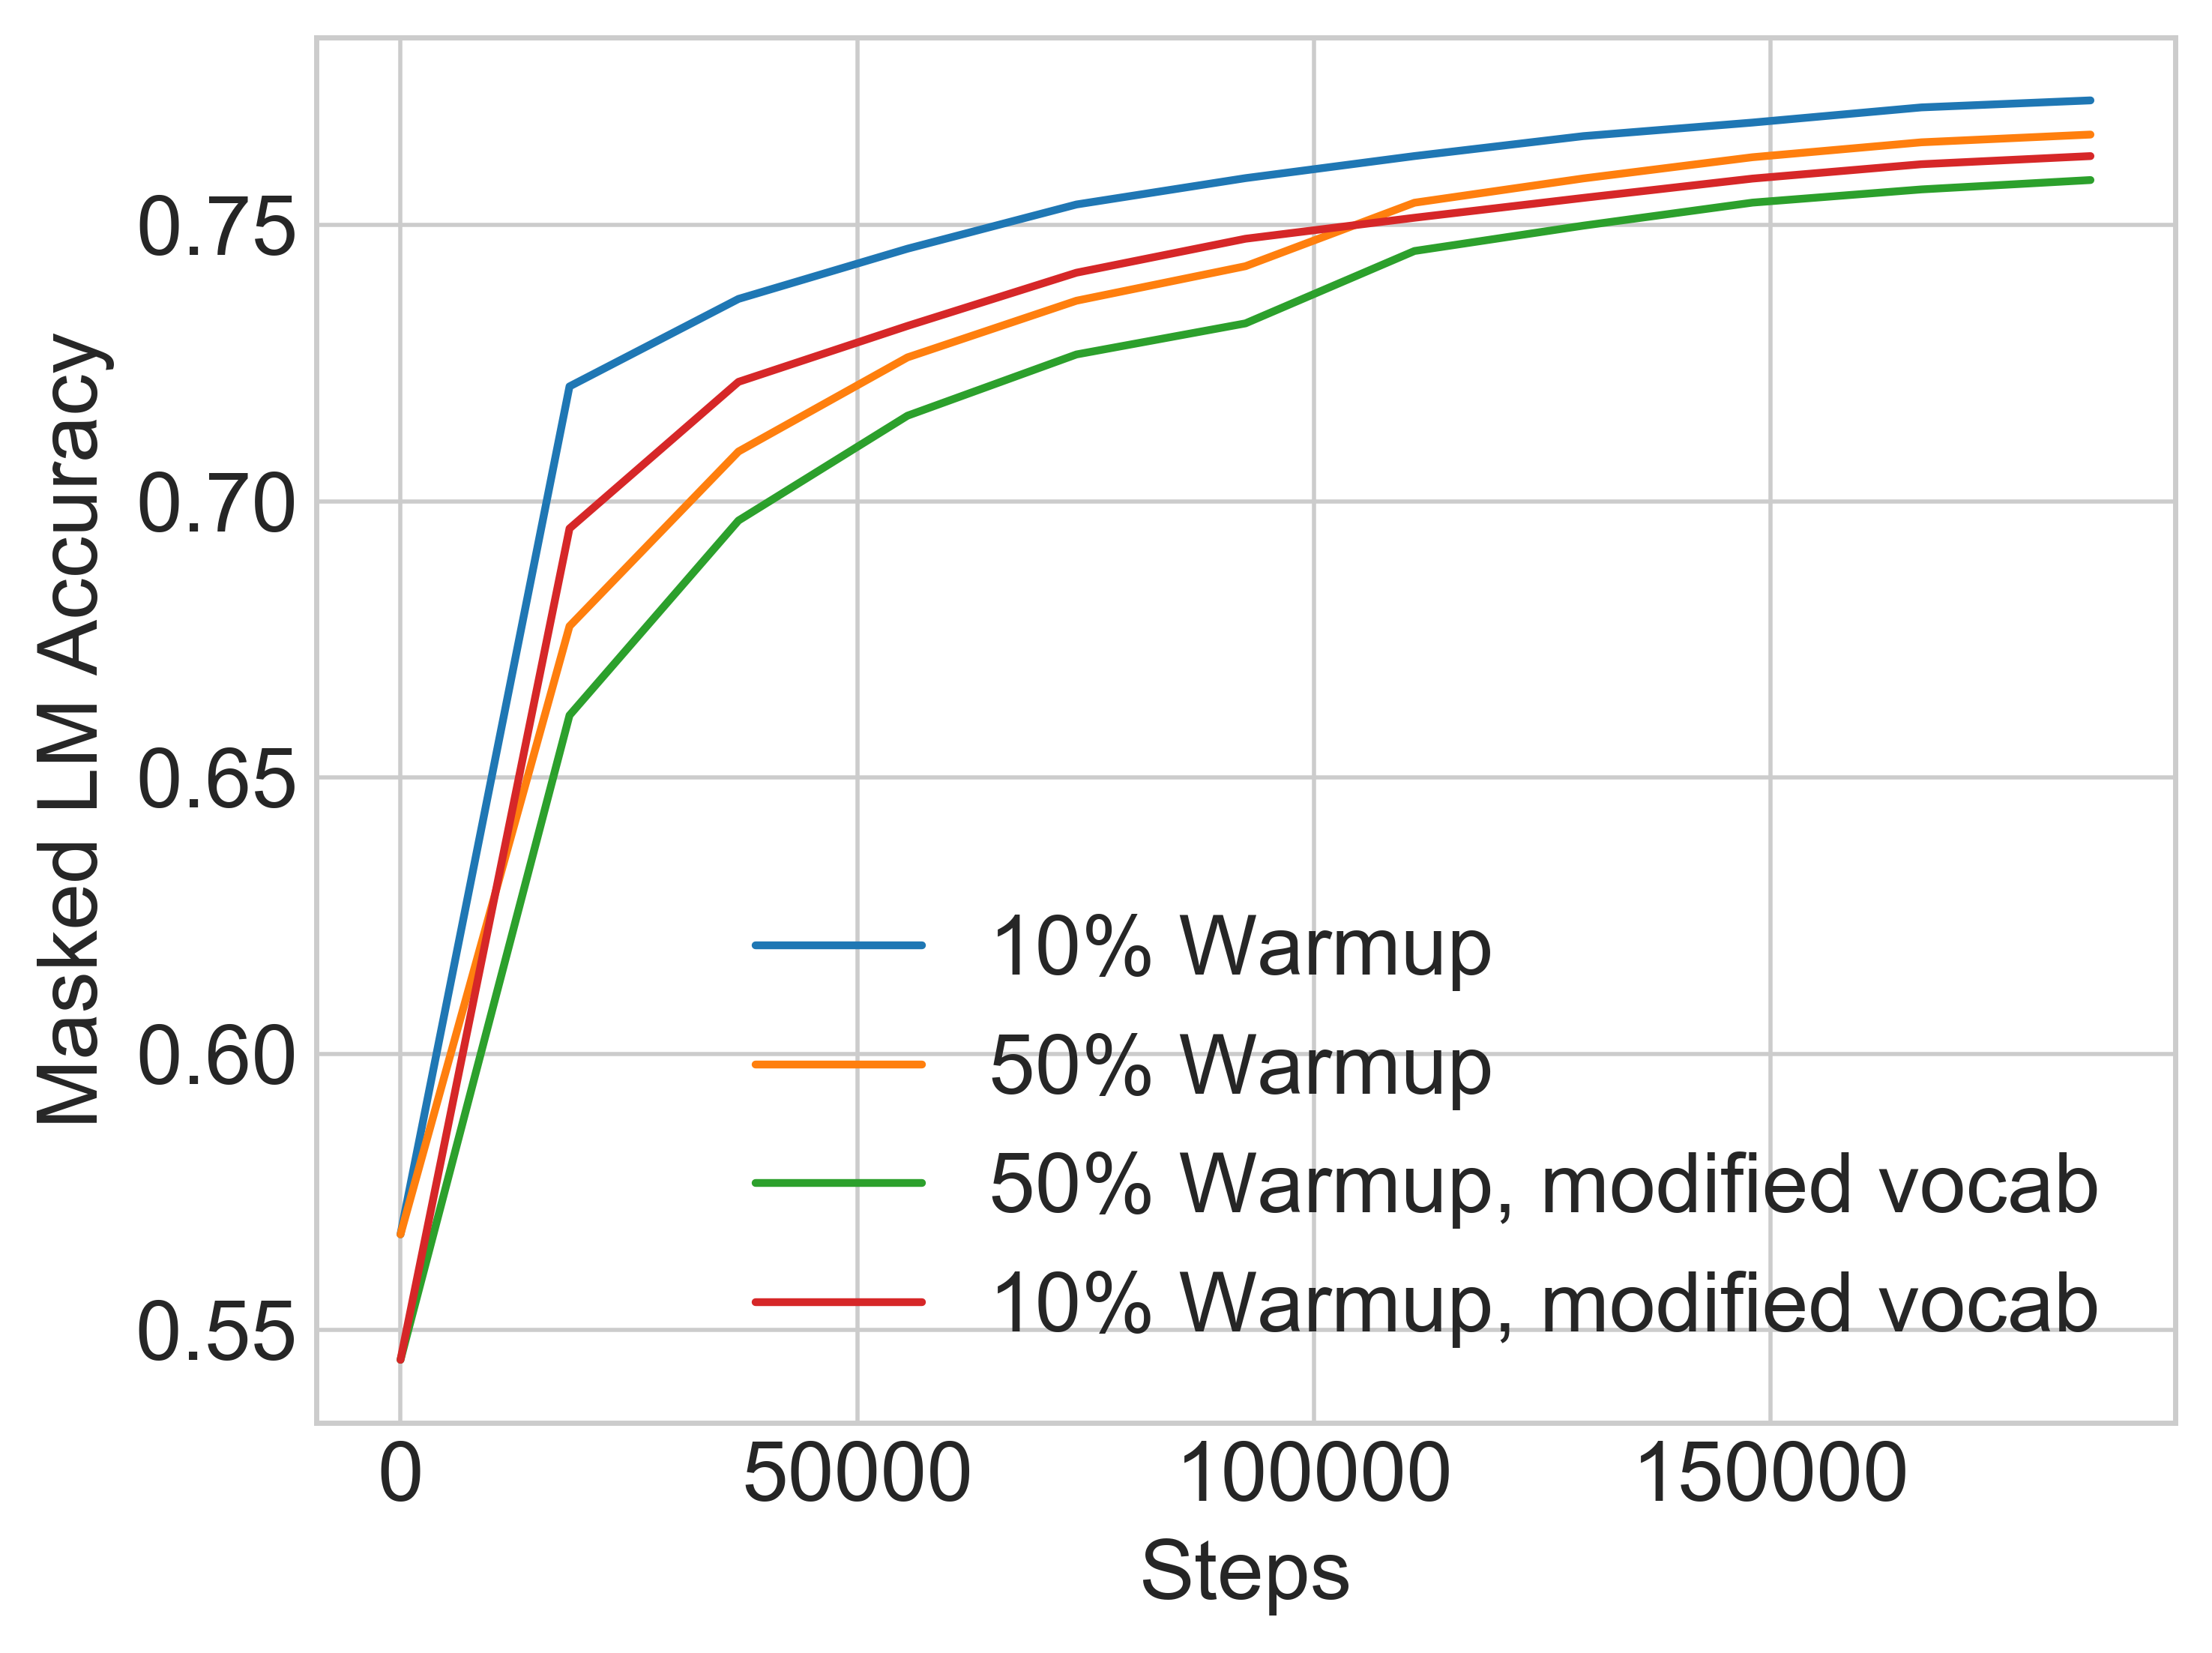
\includegraphics[width=\textwidth]{figures/charts/pretraining_learning.png}
        \caption{Masked language model.}
        \label{figure:bert_pretraining_learning_mlm}
    \end{subfigure}
    \begin{subfigure}{0.5\textwidth}
        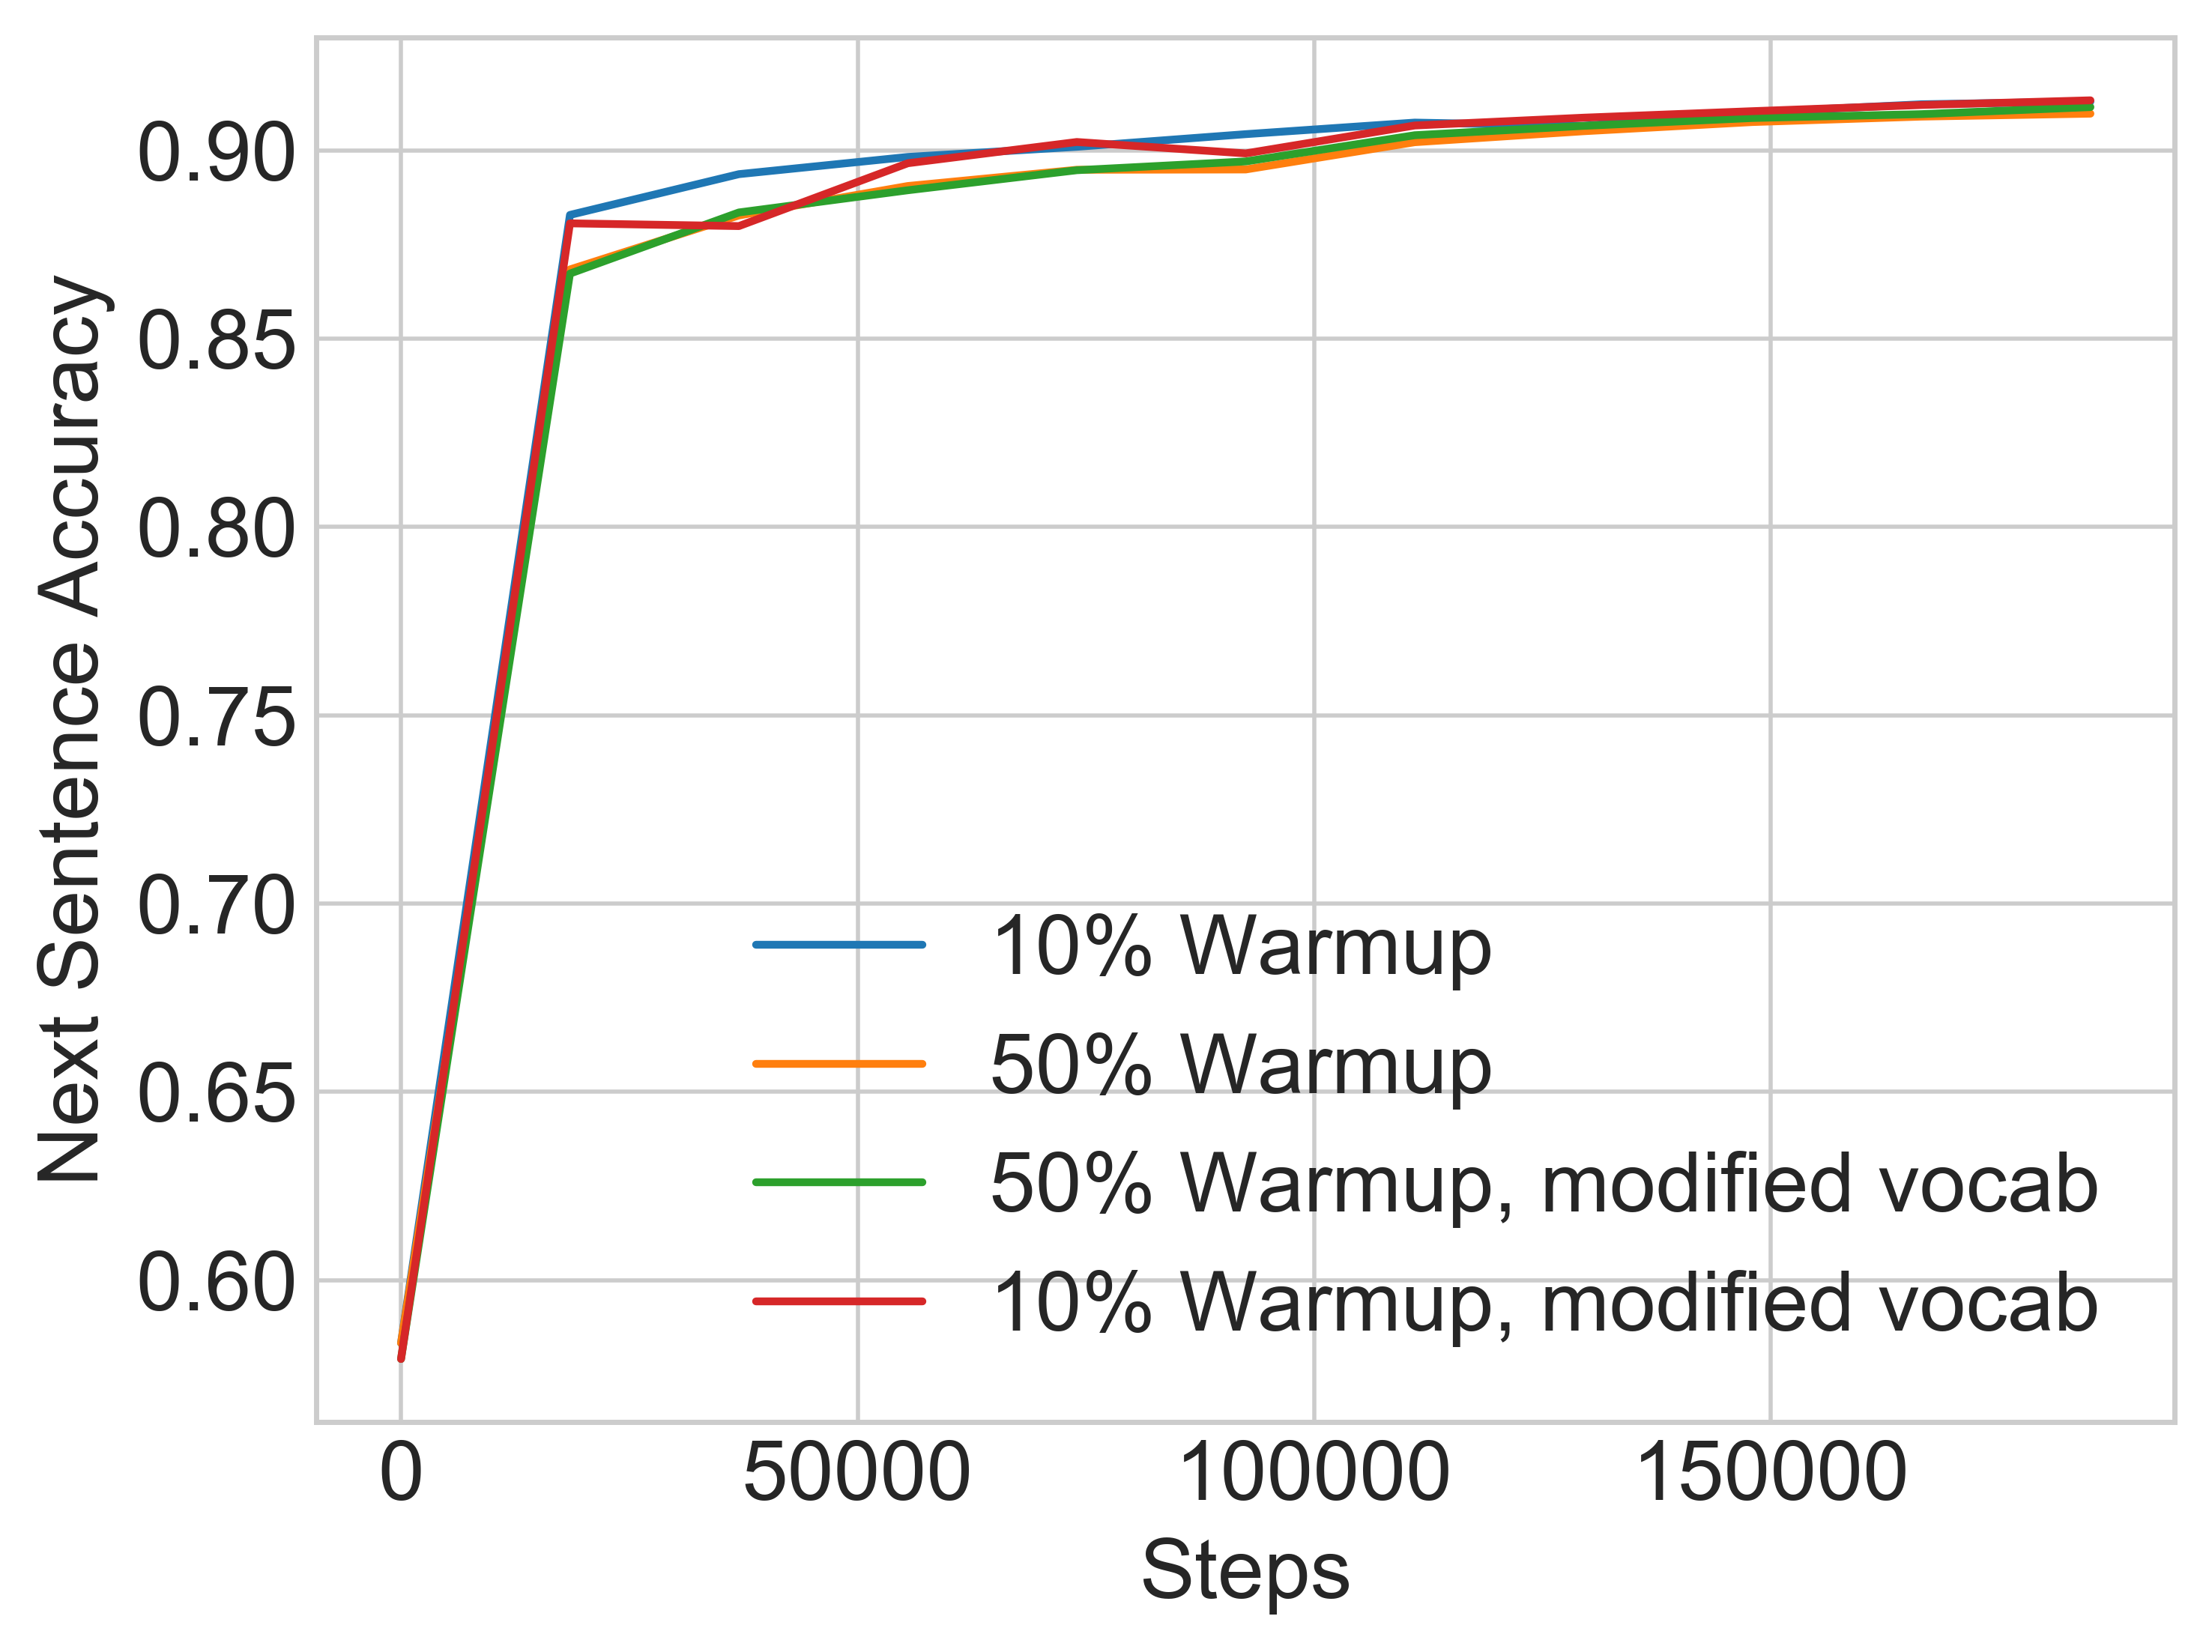
\includegraphics[width=\textwidth]{figures/charts/pretraining_learning_nsp.png}
        \caption{Next sentence prediction.}
        \label{figure:bert_pretraining_learning_nsp}
    \end{subfigure}
    \caption{Learning curves of the \ac{BERT} pretraining step.}
    \label{figure:bert_pretraining_learning}
\end{figure}
One attempt to improve this accuracy was to use a different warmup rate.
\cite{Popel2018} find that the transformer architecture is sensitive to the number of warmup steps.
A short warmup phase can therefore lead to \textit{diverged} training, where the learning curve drops almost to zero and does not recover \cite[p. 60]{Popel2018}.
Even if that is not the same behavior as observed here, it is an indicator that the accuracy might be affected by the short warmup rate of 10\% of the total training steps.
However, the masked LM accuracy could not be improved with setting the warmup steps to 92500 as the orange curve shows (76.6\% on the validation dataset).
Another idea was that the vocabulary of \ac{BERT} might not be appropriate to model the language of business reports.
Since BERT was trained on Wikipedia articles, a lot of special finance or accounting terms are not covered by the vocabulary.
Therefore these terms have to be split up by \ac{BERT} into sub-tokens, which can lead to bad word representations.
For example the term \textit{liabilities} was split up into \textit{lia} and \textit{\#\#bilities} or \textit{deferred} was split into \textit{def}, \textit{\#\#erre} and \textit{\#\#d}.
These two terms however already account for 1\% of all words in the dataset (train, validation and test combined).
Table \ref{table:not_in_vocab_words} shows the ten most frequent words, that had to be split up in sub-tokens, because they can't be represented by a single token from the vocabulary.
\begin{table}[h]
    \centering
    \begin{tabular}{ c  c  c }
        Word & Tokenization & Proportion of all words in dataset \\ \hline
        liabilities & lia \#\#bilities & 0.65\% \\
        deferred & def \#\#erre \#\#d & 0.32\% \\
        liquidity & liquid \#\#ity & 0.23\% \\
        repurchase & rep \#\#ur \#\#chase & 0.23\% \\
        adversely & adverse \#\#ly & 0.21\% \\
        intangible & int \#\#ang \#\#ible & 0.20\% \\
        materially & material \#\#ly & 0.19\% \\
        amortization & amor \#\#ti \#\#zation & 0.19\% \\
        borrowings & borrowing \#\#s & 0.19\% \\
        registrant & regis \#\#tra \#\#nt & 0.18\% \\
    \end{tabular}
    \caption{The most common words, that can't directly be represented by a token from the vocabulary.}
    \label{table:not_in_vocab_words}
\end{table}
It seems obvious that the accuracy is affected, if these words are often used and have a bad representation by the tokens in the vocabulary.
Therefore these words should also be incorporated in the vocabulary.
However, building a vocabulary based on the business reports has the drawback that the pre-trained checkpoints released by Google can not be reused.
Pre-training from scratch takes about two weeks on a Google Cloud TPU and even longer on a GPU\footnote{\url{https://github.com/google-research/bert\#pre-training-tips-and-caveats}}, which eliminates this option because of the limited time scope of the research.
The developers of \ac{BERT} anticipated this situation and left 994 tokens unused which can be set to custom words.
These were set to the words that occur more than 100000 times in the dataset, which are for example "liabilities", "amortization" or "depreciation".
As the green and the red curve in figure \ref{figure:bert_pretraining_learning_mlm} show, this even has a negative effect on the masked LM accuracy, because \ac{BERT} first has to learn the meaning of the words.
Even though the accuracy then improves, it always stays below the accuracy of the original vocab, with the same warmup rate.
The accuracy of the next sentence prediction showed no significant changes during these attempts as figure \ref{figure:bert_pretraining_learning_nsp} shows.

After pretraining with a sequence length of 128 tokens, \ac{BERT} was pretrained for another 18500 steps with a sequence length of 512 tokens.
% This is recommended to learn positional embeddings \cite[p. 13]{Devlin2018}.
Even though this is recommended for learning positional embeddings \cite[p. 13]{Devlin2018}, this step was first skipped, but added later again after the first fine-tuning results with a sequence length of 128 tokens were not promising (Section \ref{sec:fine_tuning_results}).
The training was continued from the checkpoint with the warmup proportion of 10\% (blue curves in Figure \ref{figure:bert_pretraining_learning}).
Figure \ref{figure:bert_pretraining_learning_512} shows the combined learning curve with a sequence length of 128 tokens to 185000 steps and 512 tokens for the last 18500 steps.
\begin{figure}[h]
    \begin{subfigure}{0.5\textwidth}
        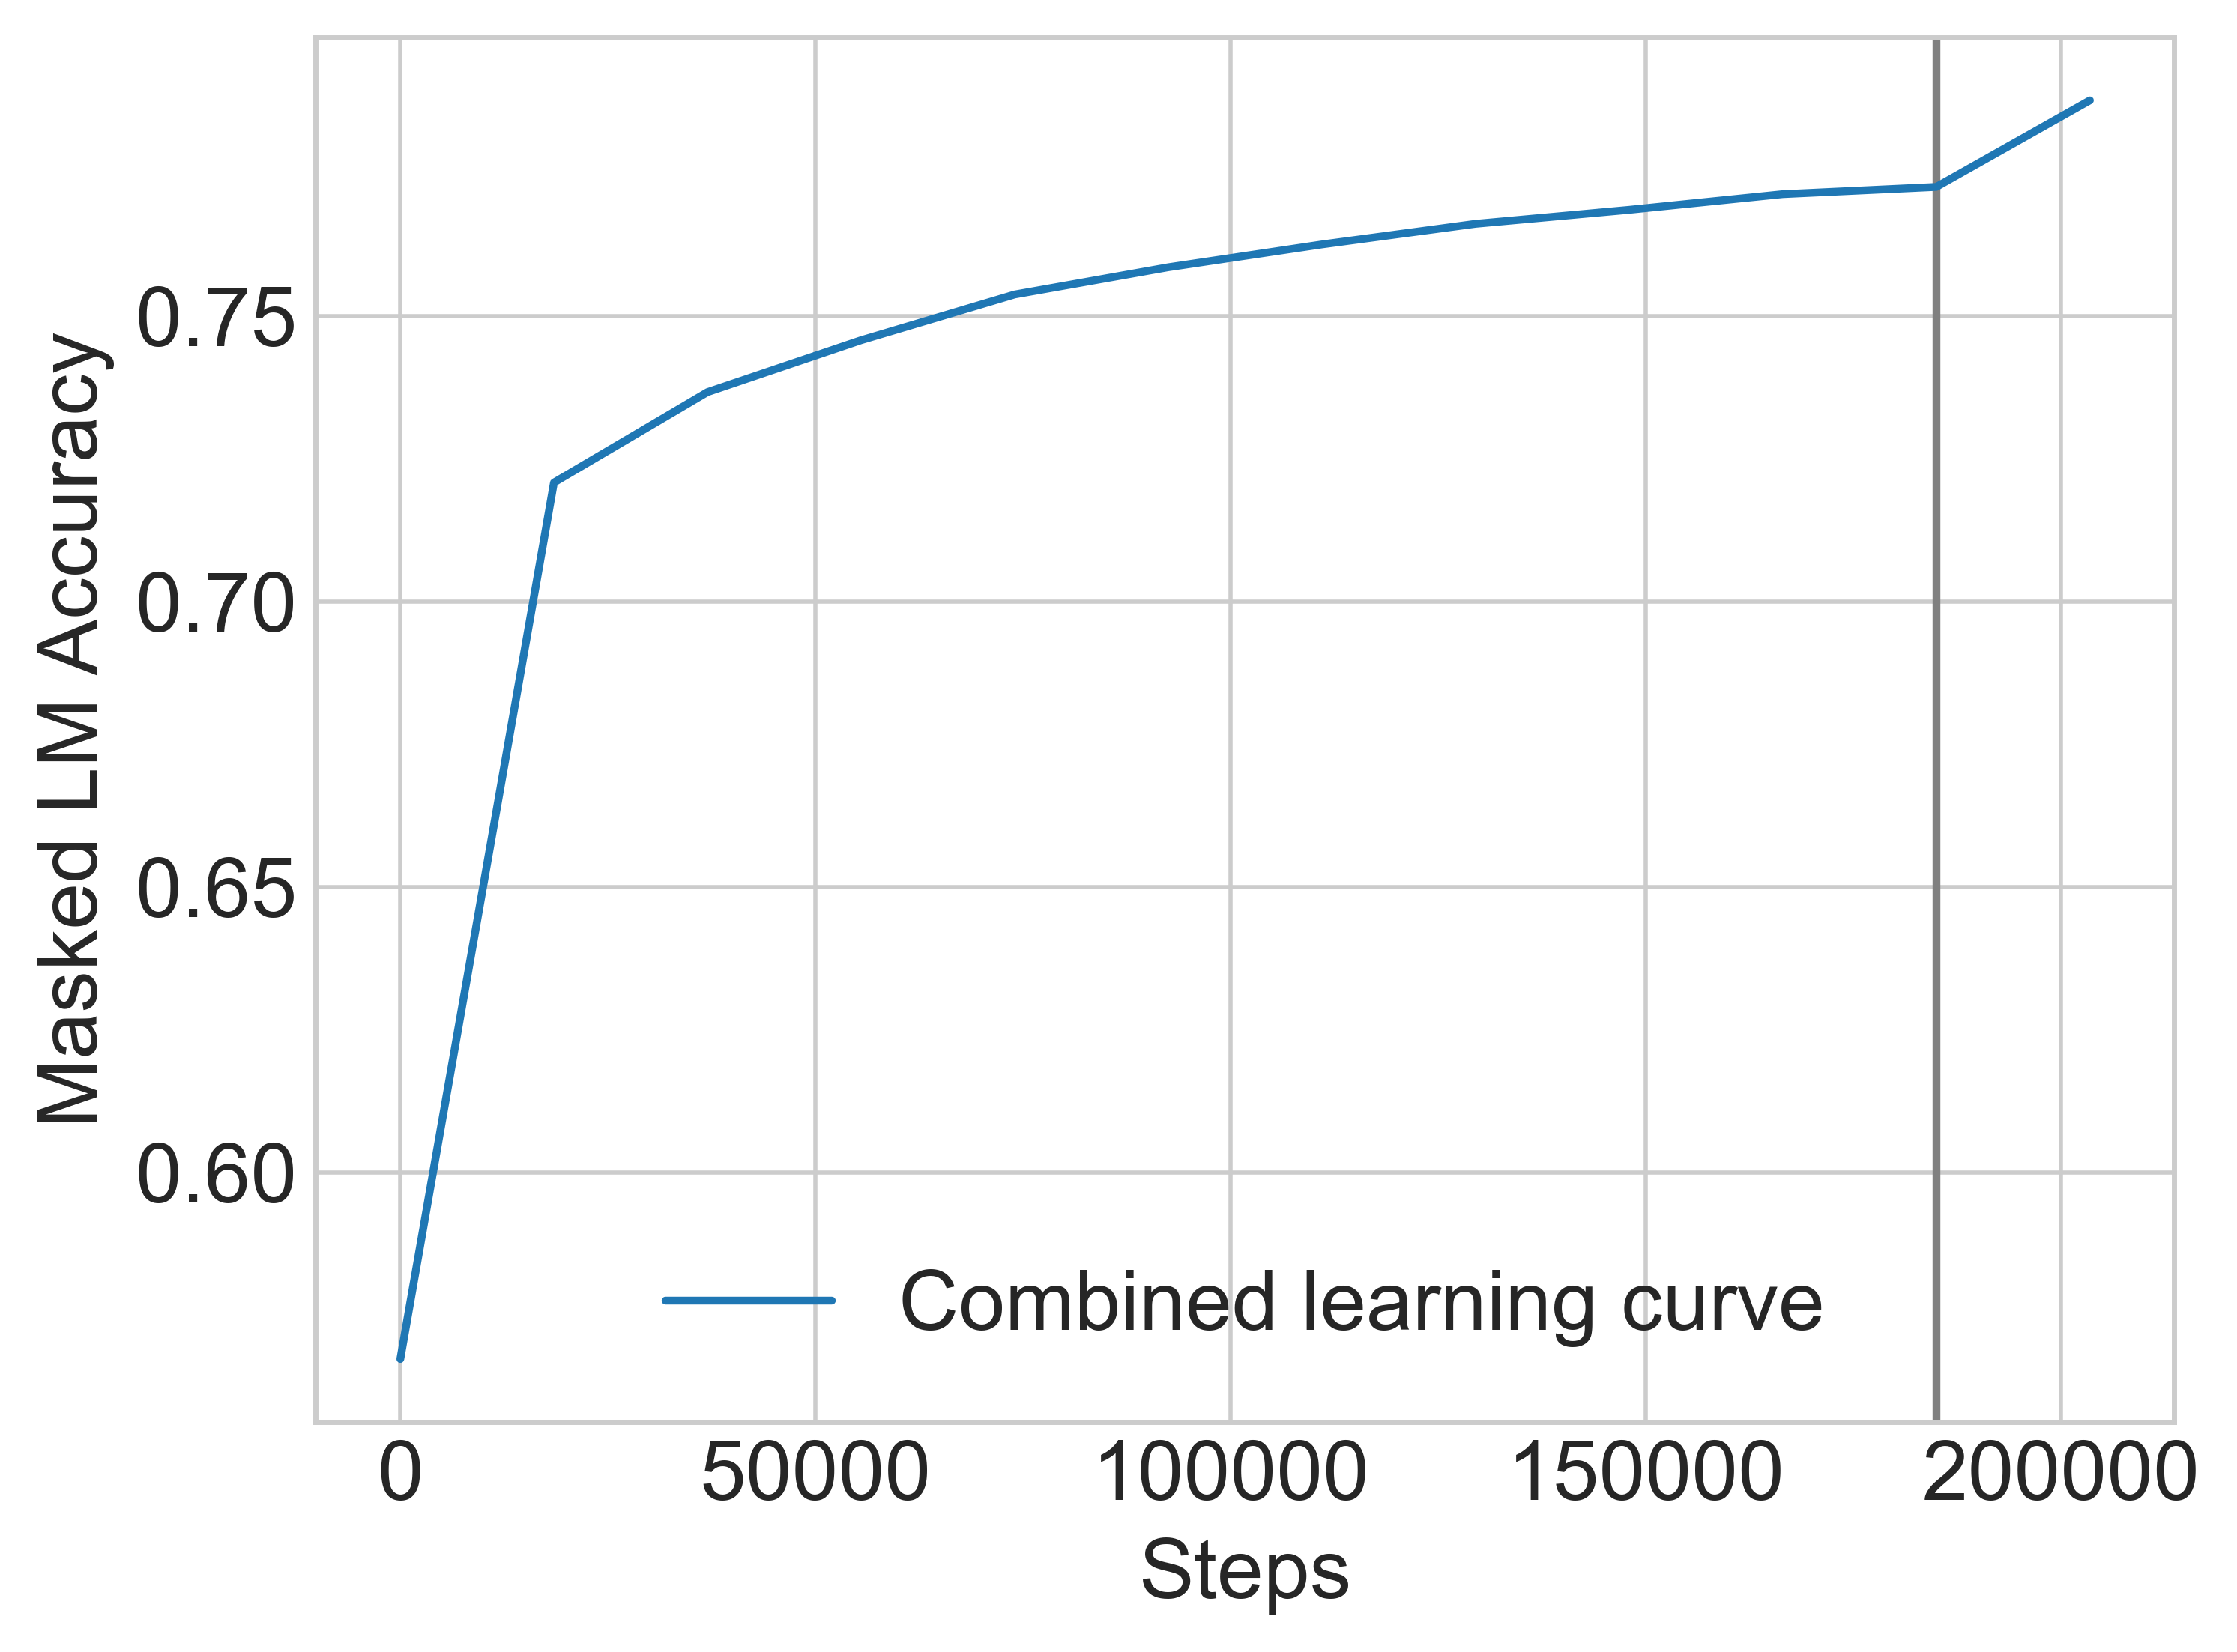
\includegraphics[width=\textwidth]{figures/charts/pretraining_learning_512.png}
        \caption{Masked language model.}
        \label{figure:bert_pretraining_learning_512_mlm}
    \end{subfigure}
    \begin{subfigure}{0.5\textwidth}
        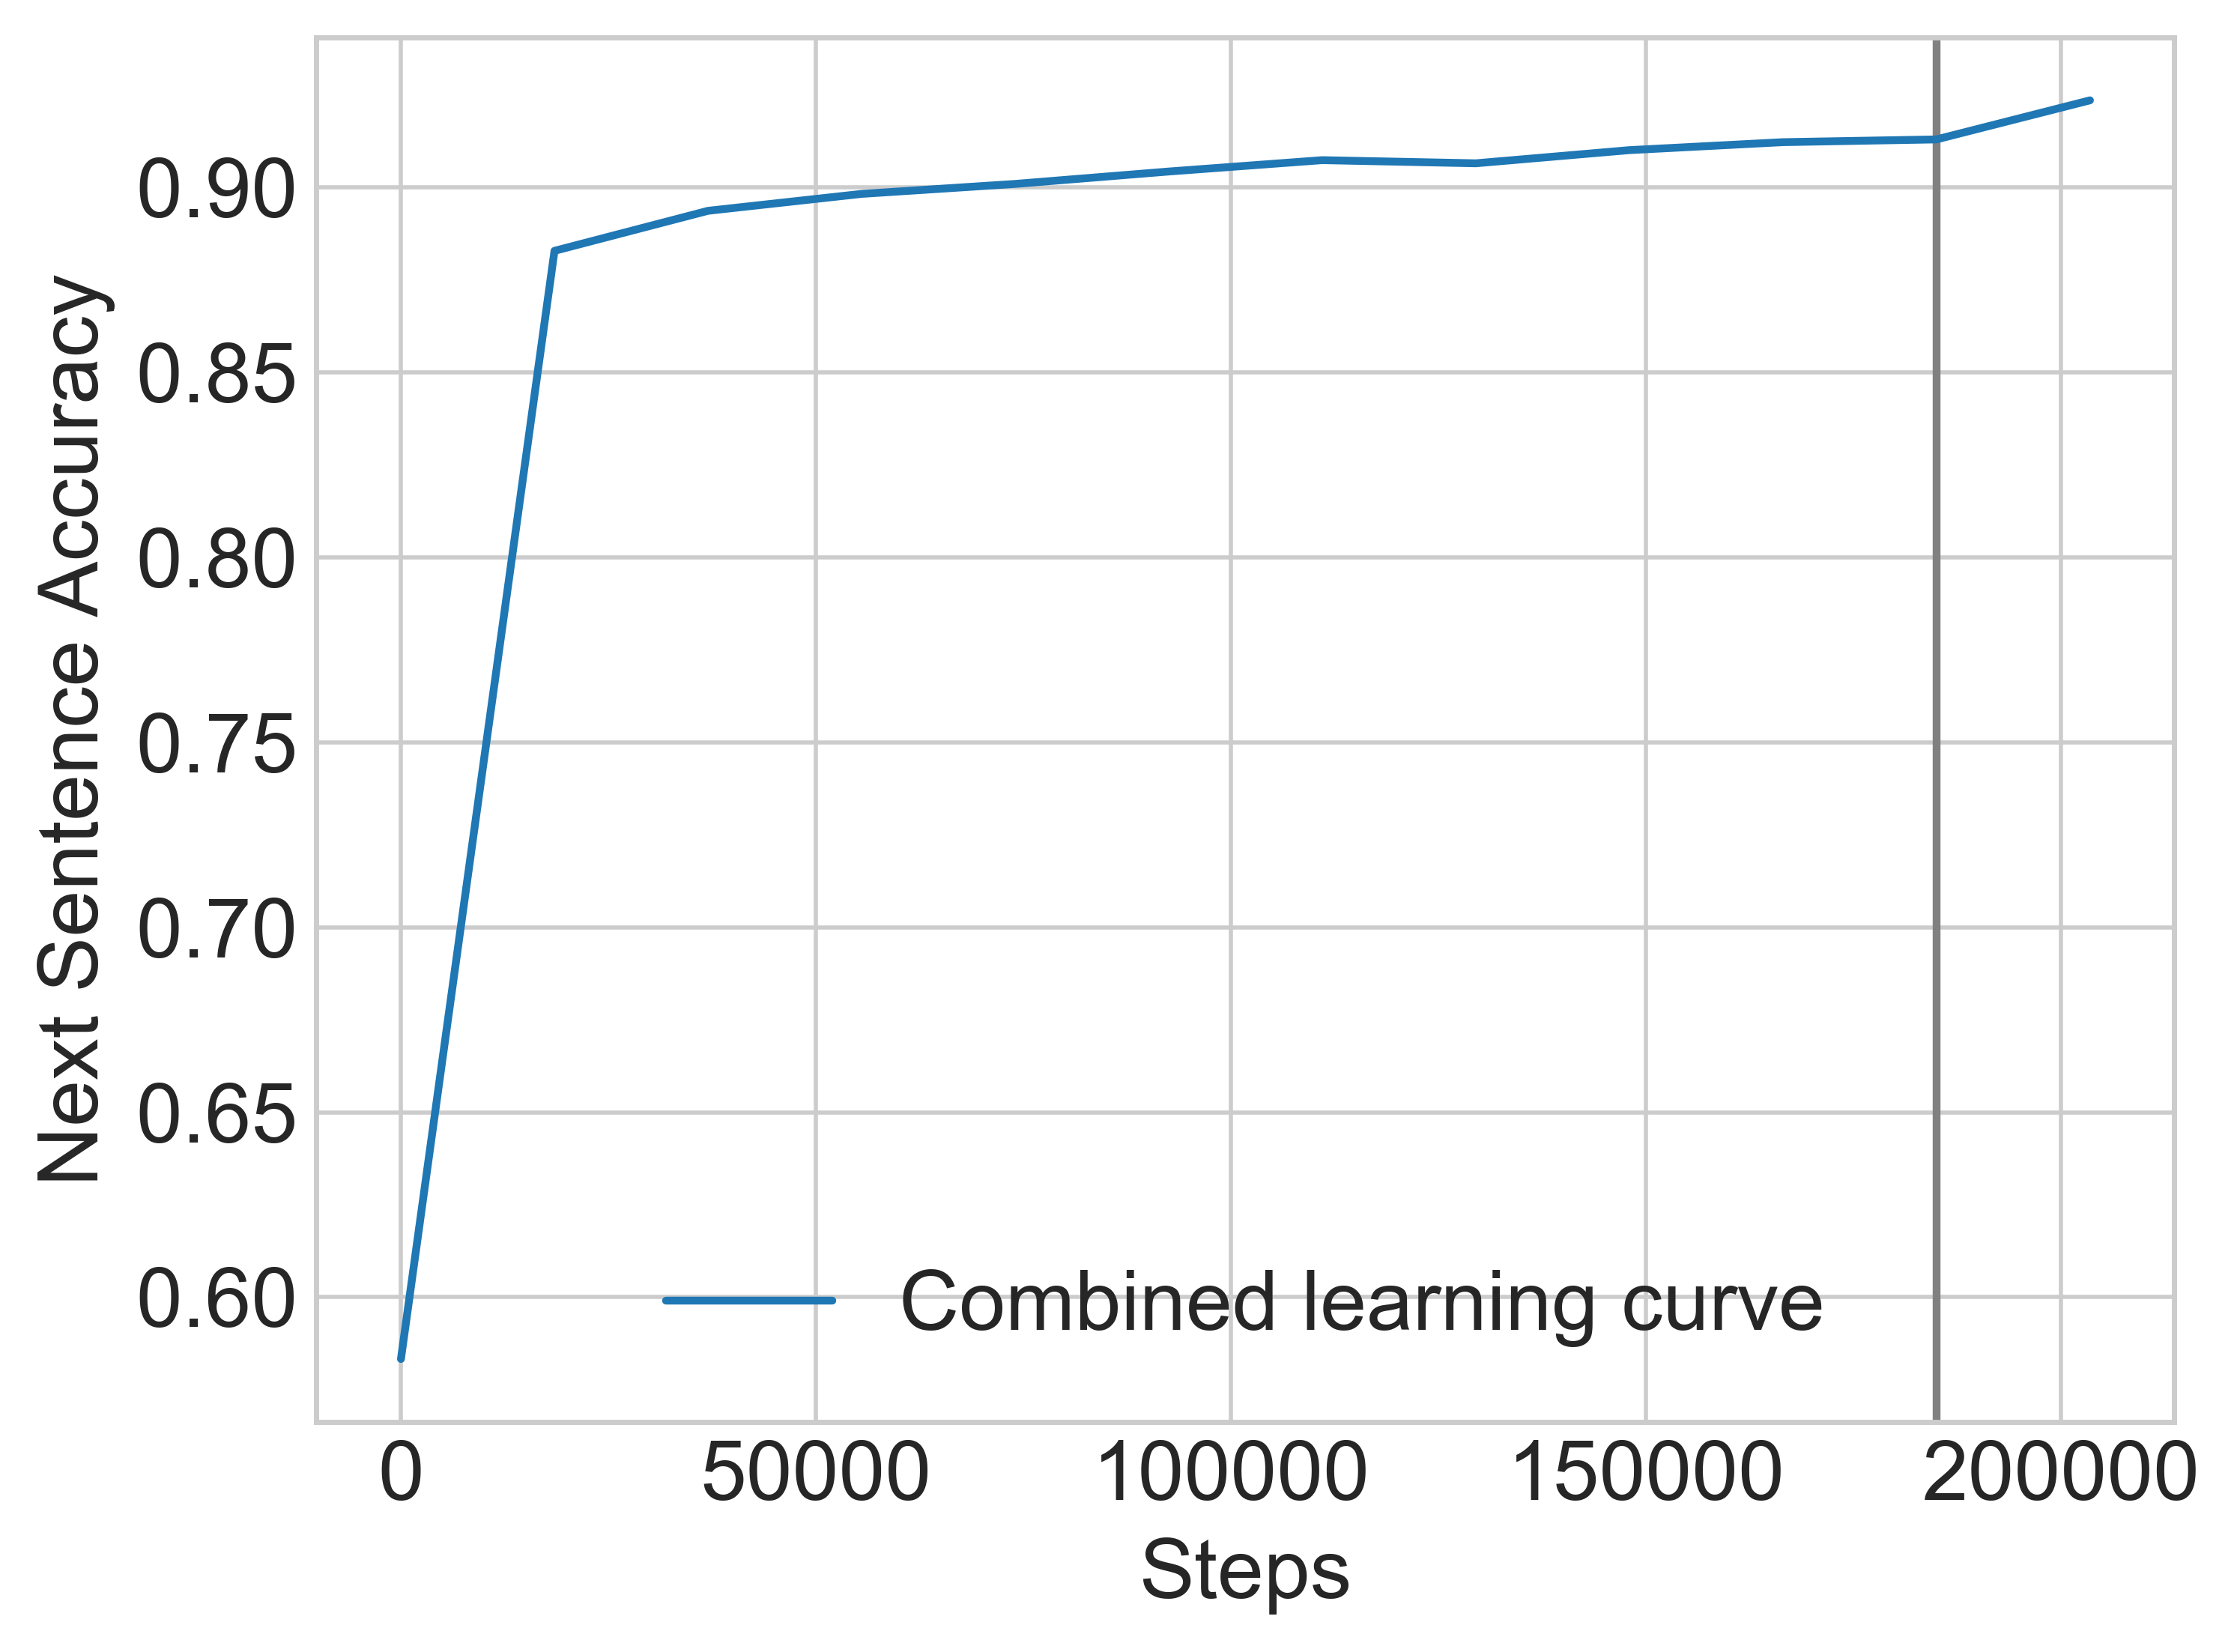
\includegraphics[width=\textwidth]{figures/charts/pretraining_learning_512_nsp.png}
        \caption{Next sentence prediction.}
        \label{figure:bert_pretraining_learning_512_nsp}
    \end{subfigure}
    \caption{Combined learning curves of the sequence length 128 and 512.}
    \label{figure:bert_pretraining_learning_512}
\end{figure}
It can be seen, that the longer sequences improve both the masked LM accuracy and the next sentence prediction accuracy by a significant amount.
The final masked LM accuracy on an independent test dataset was 79.1\% and for the next sentence prediction 92.2\% was reached.
These results are really similar to the results of FinBERT which was also trained on Form 10-K filings \cite[p. 4]{DeSola2019}.
They carried out a pre-training from scratch and gained a masked LM accuracy of 80.17\% and a next sentence prediction accuracy of 98.5\% \cite[p. 7]{DeSola2019}.
The model that was trained on top of the Google checkpoint achieved a masked LM accuracy of 77.2\% and a next sentence prediction accuracy of 90.63\% \cite[p. 7]{DeSola2019}.

Pre-training was run on one NVIDIA GeForce RTX 2080 Ti and took about 19 hours for the training with sequence length 128 and about 2 hours for learning the positional embeddings, with a sequence length of 512 tokens.

\section{Classification}
\label{sec:report_classification}

\subsection{Fine-tuning \ac{BERT}}
\label{sec:fine_tuning_results}
With the fine-tuning, \ac{BERT} is trained to classify the input sequences.
In the case of this research the input sequences are the sentences obtained from spaCy with the label \textit{positive} or \textit{negative} (Section \ref{subsec:fine_tuning}).
As described in the previous section \ref{sec:pre_training_results} the fine-tuning was first executed from the pre-training checkpoint with a sequence length of 128 tokens and a warmup rate of 10\%.
That resulted in the blue curve in figure \ref{figure:bert_finetuning_learning} as the learning progress.
\begin{figure}[h]
    \centering
    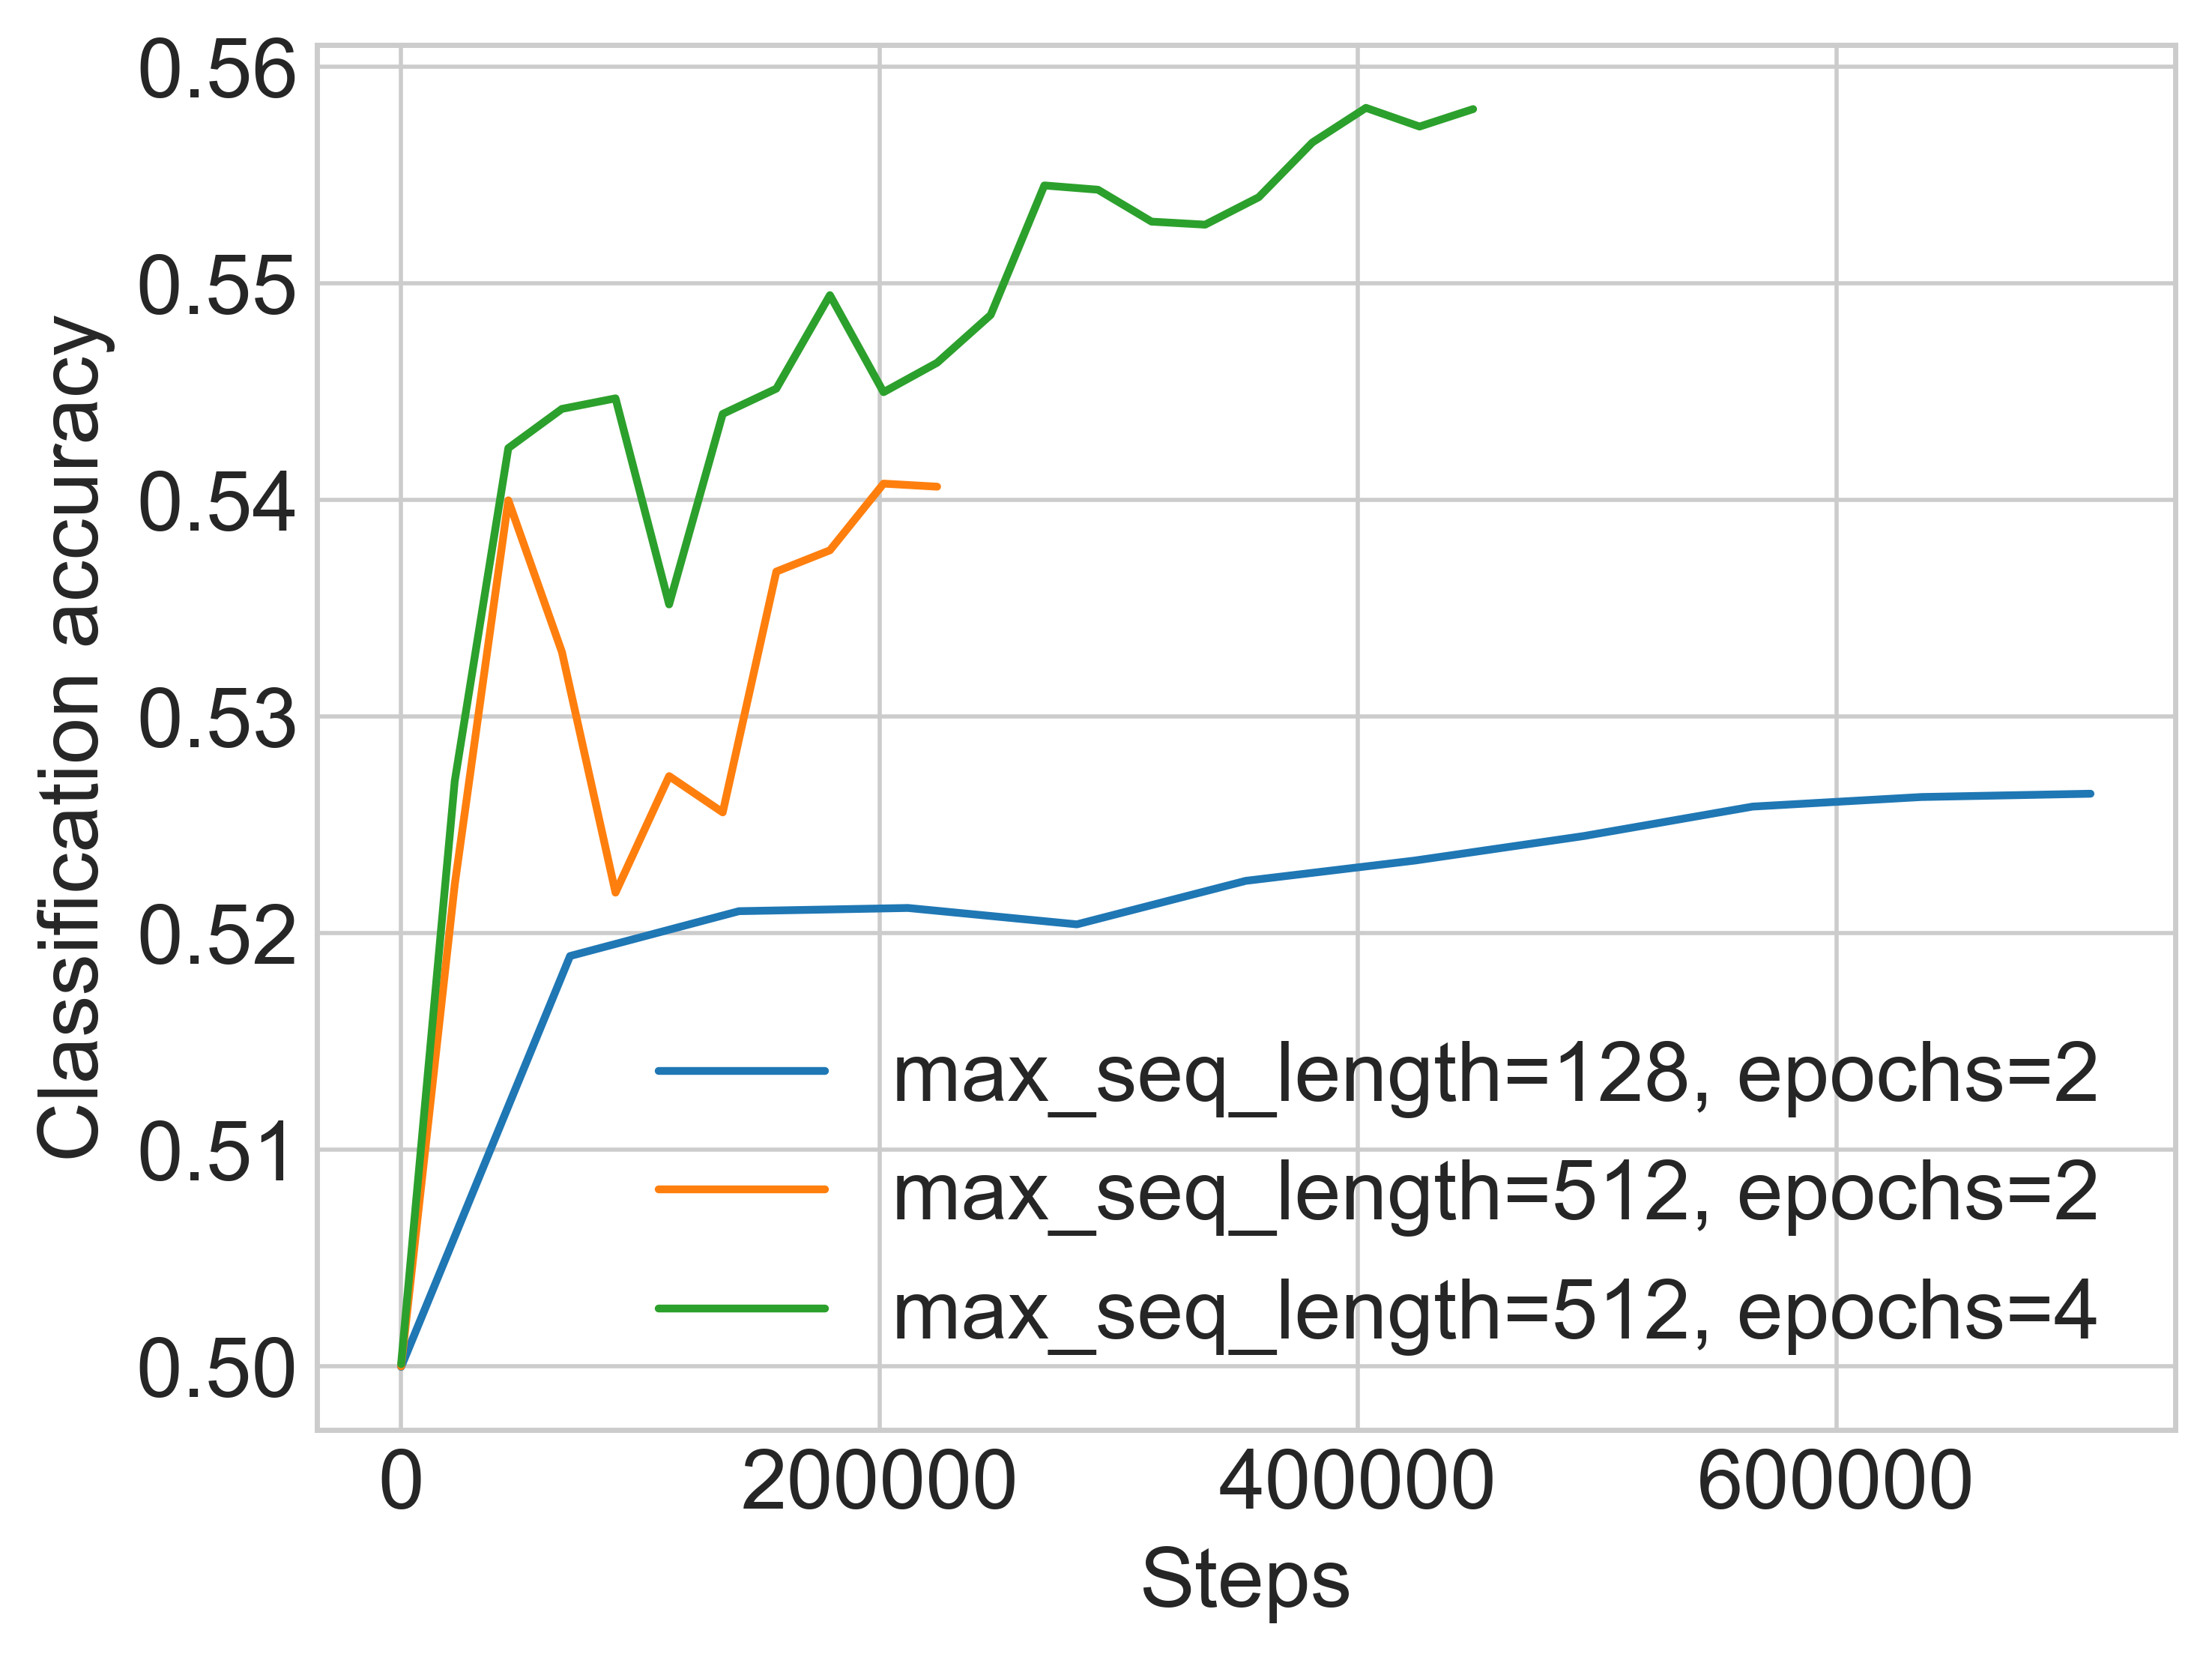
\includegraphics[width=0.5\textwidth]{figures/charts/finetuning_learning.png}
    \caption{Learning curve for finetuning \ac{BERT}.}
    \label{figure:bert_finetuning_learning}
\end{figure}
The classification accuracy of 52.6\% on the validation dataset is of course not an acceptable performance, considering that random guessing on two classes gives a mean accuracy of 50\%.
This low accuracy results from the low sequence length of 128 tokens.
These short sequences are not really representative for a whole business report.
Only if the sequences are combined to longer text segments, they give more evidence about the market reaction that the underlying business report created, as the next experiment confirms.
For that the sequence length was set to 512 tokens and the pretraining checkpoint with a sequence length of 512 tokens was used.
This leads to an improvement of 1.4\%, if the number of epochs is set to 2 and to an improvement of 3.17\%, if the number of epochs is set to 4.
Furthermore, it it is also noteworthy, that the number of epochs has a direct effect on the accuracy, which is not caused by the longer training time.
Even after the same training steps, the accuracy of the model with a training duration of four epochs, is higher than the accuracy of the model with a training duration of two epochs.
Because the data and all other parameters remained unchanged, this difference can be traced back to the number of warmup steps.
Since the number of warmup steps is set as a proportion of 10\% of the total training steps, it also increases if the training duration is set higher
The model that trained 4 epochs was then used to extract the hidden states as the report features.
This gave a classification accuracy on an independent test dataset of 55.4\%, and took 45 hours to train.

\subsection{Naive Bayes}
\label{subsec:nb_results}
The first classifier that was tested with the extracted hidden states from \ac{BERT} was a Naive Bayes classifier.
As described in section \ref{subsec:methods_for_document_representation}, \ac{BERT} can process the reports only sequence by sequence which results in multiple embedding vectors for one report.
For the Naive Bayes classifier the report has to be represented by only one embedding vector, therefore all sequence embeddings of one report were averaged.
The learning curve for the training of the classifier is presented in figure \ref{figure:nb_learning}.
\begin{figure}[h]
    \centering
    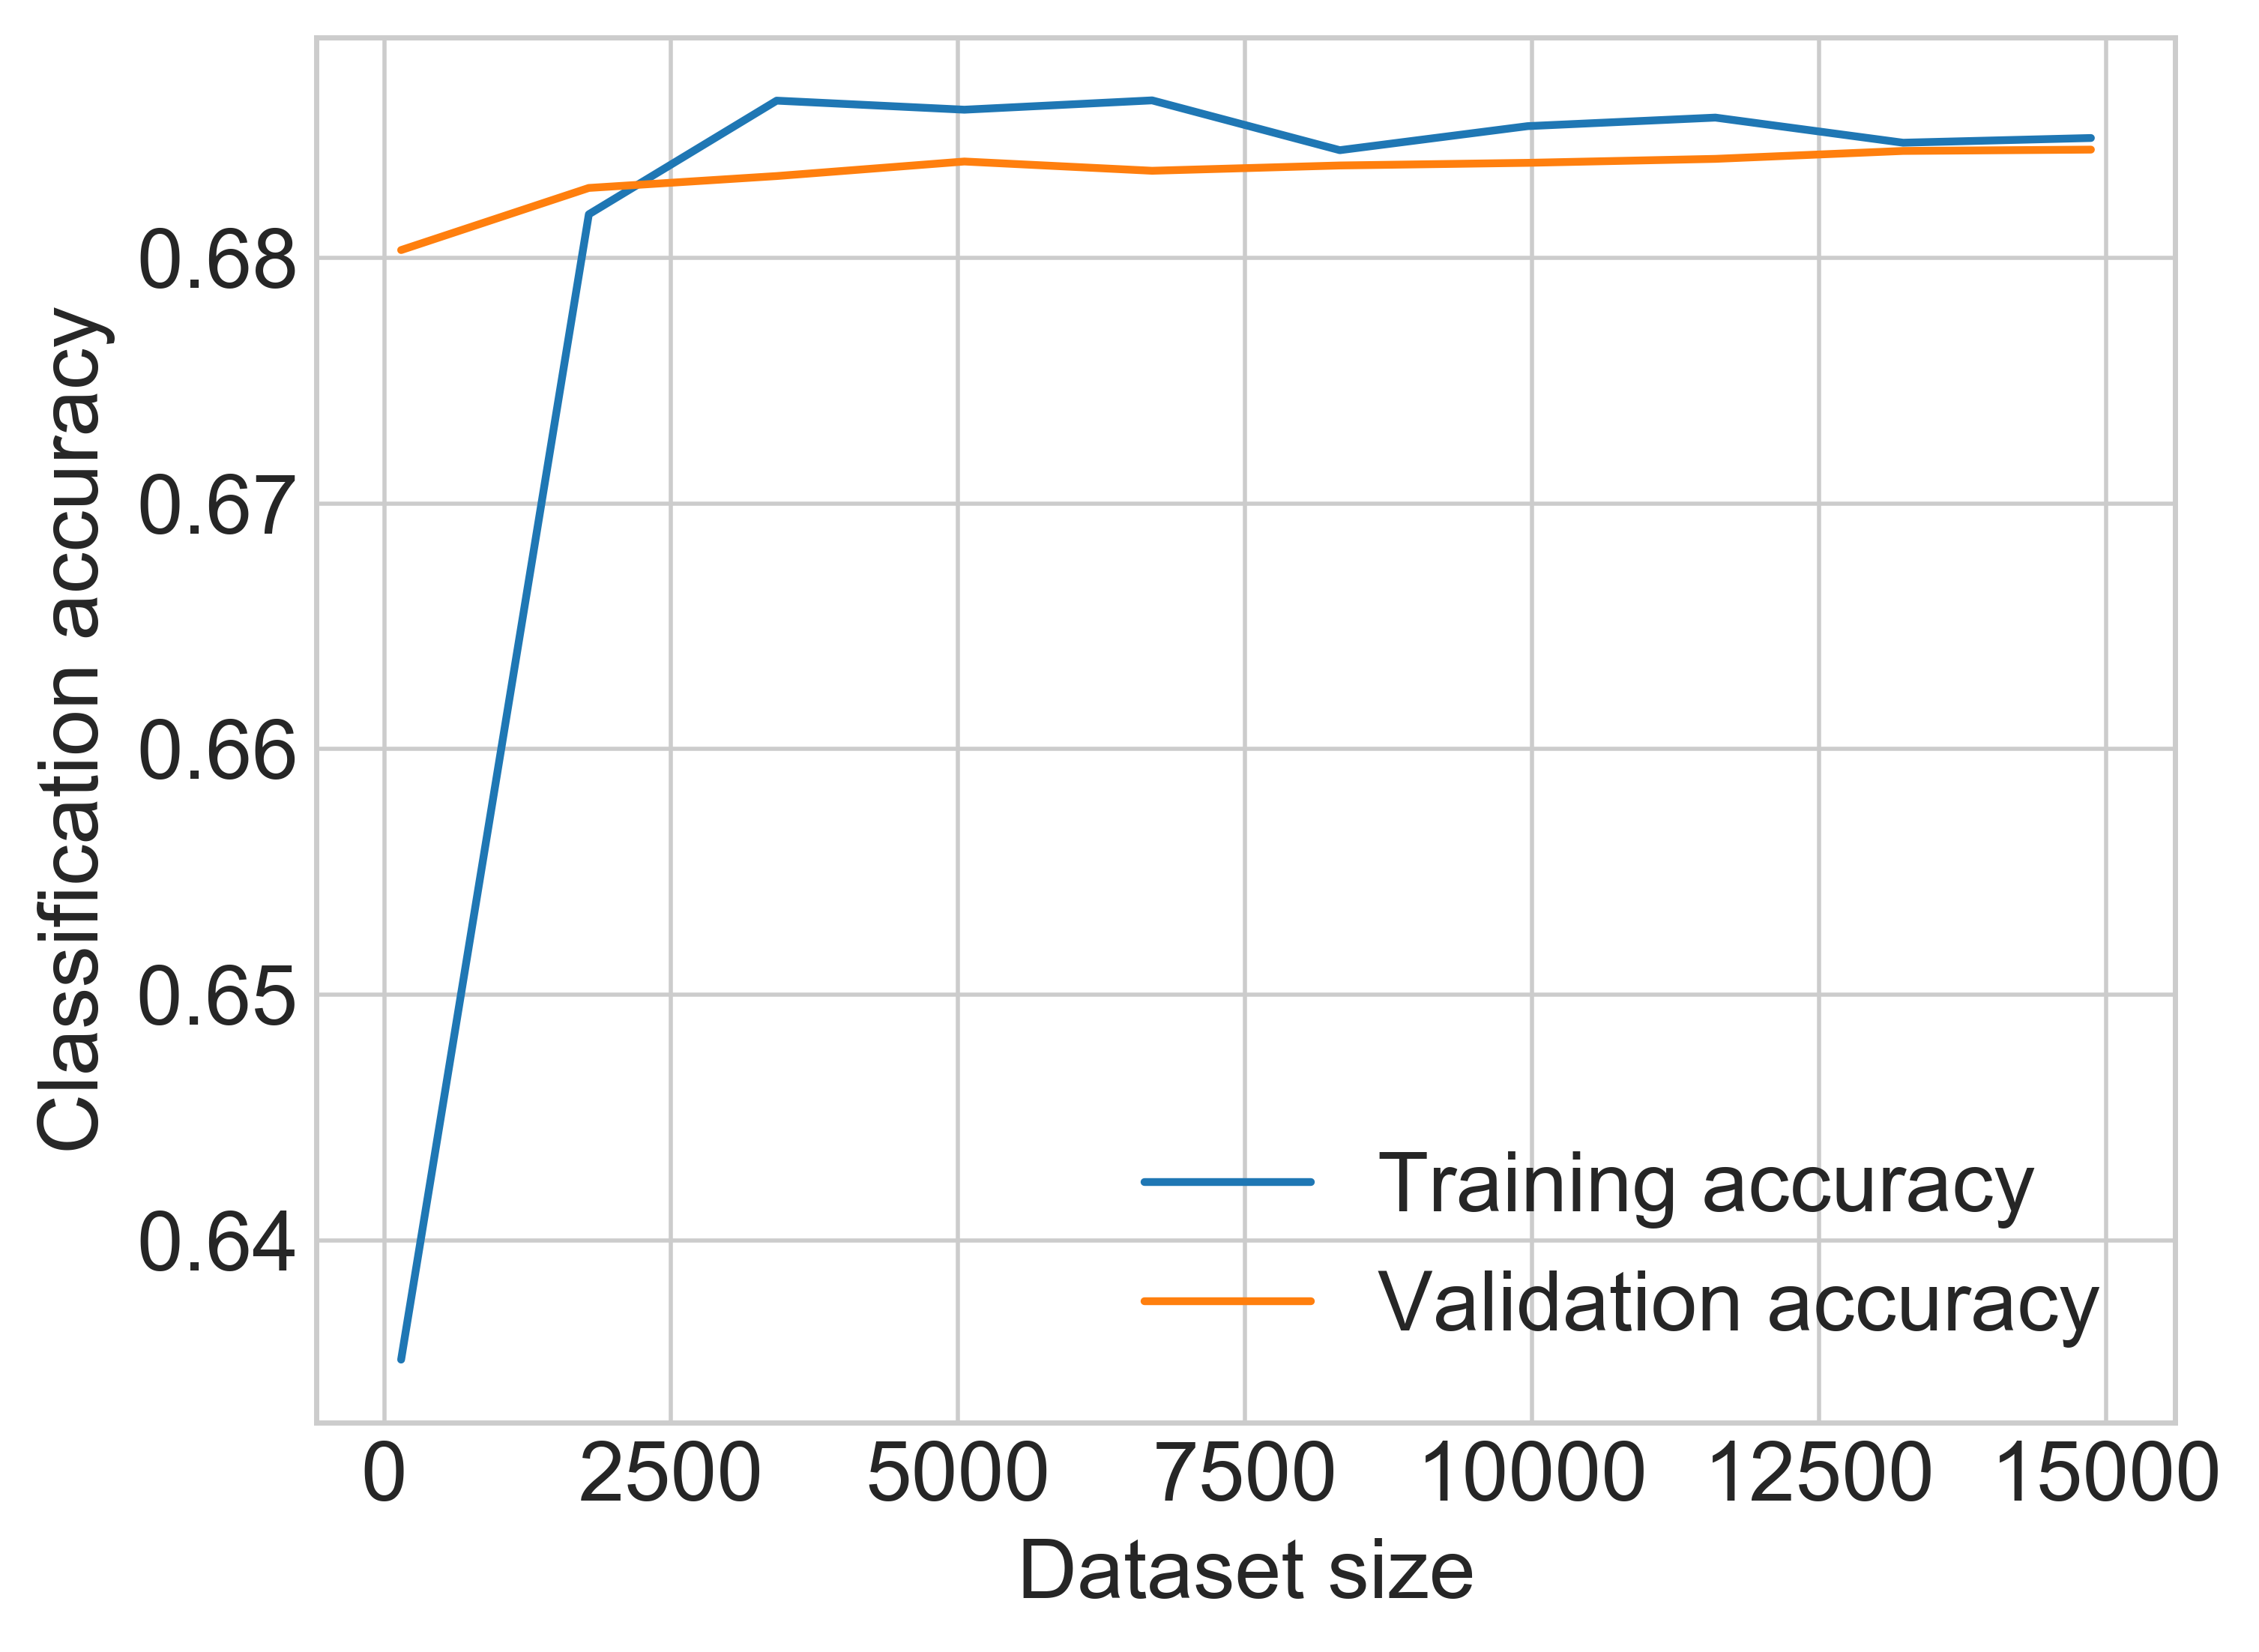
\includegraphics[width=0.5\textwidth]{figures/charts/nb_learning.png}
    \caption{Learning curve for the Naive Bayes classifier.}
    \label{figure:nb_learning}
\end{figure}
The test accuracy of the naive bayes model was 68.1\%, which is a significant improvement over the classification accuracy of single sequences during finetuning.
This improvement can be explained due to the averaging of the feature vectors of each report.
That removes random noise from the data which results from the text passages, which have no impact on the stock price.
A view on the dimension reduced data shows that positive and negative datapoints for the single sequences (figure \ref{figure:pca_sequence}) overlap each other more than for the averaged features, which represent the document (figure \ref{figure:pca_document}).
\begin{figure}[h]
    \begin{subfigure}{0.5\textwidth}
        \centering
        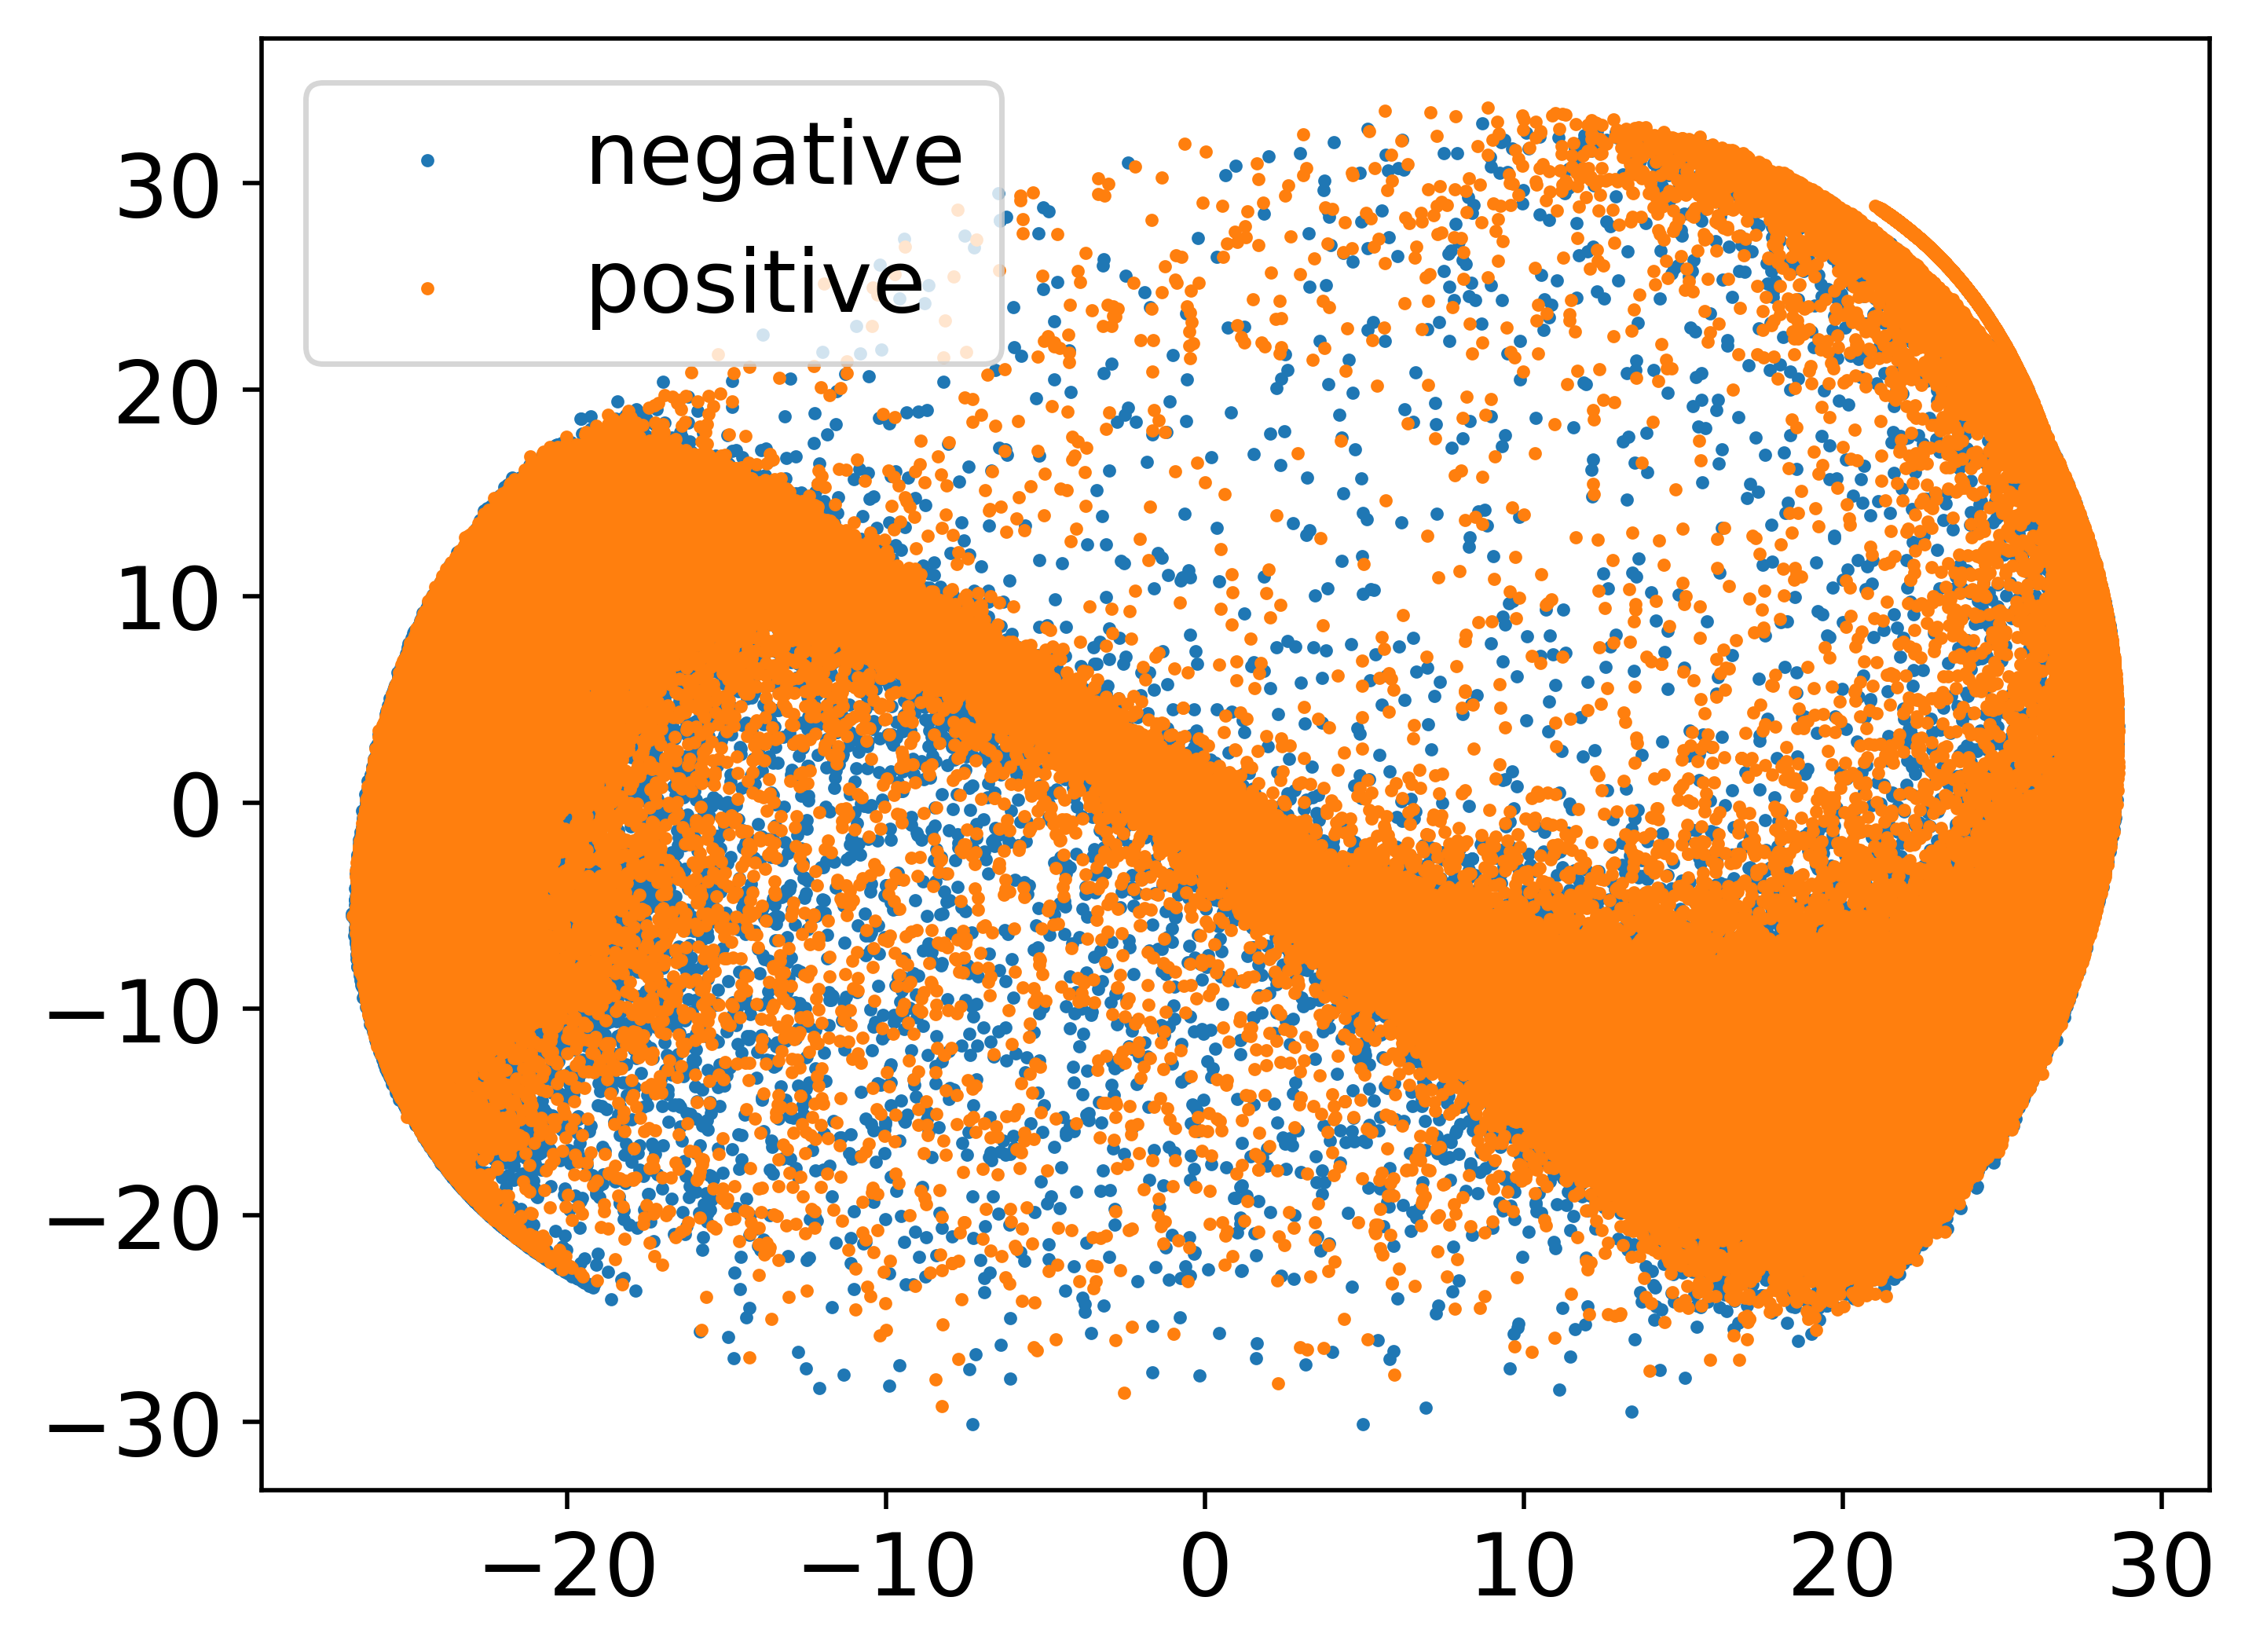
\includegraphics[width=\textwidth]{figures/pca_scatter_sequence_level.png}
        \caption{Each point represents a sequence of a document.}
        \label{figure:pca_sequence}
    \end{subfigure}
    \begin{subfigure}{0.5\textwidth}
        \centering
        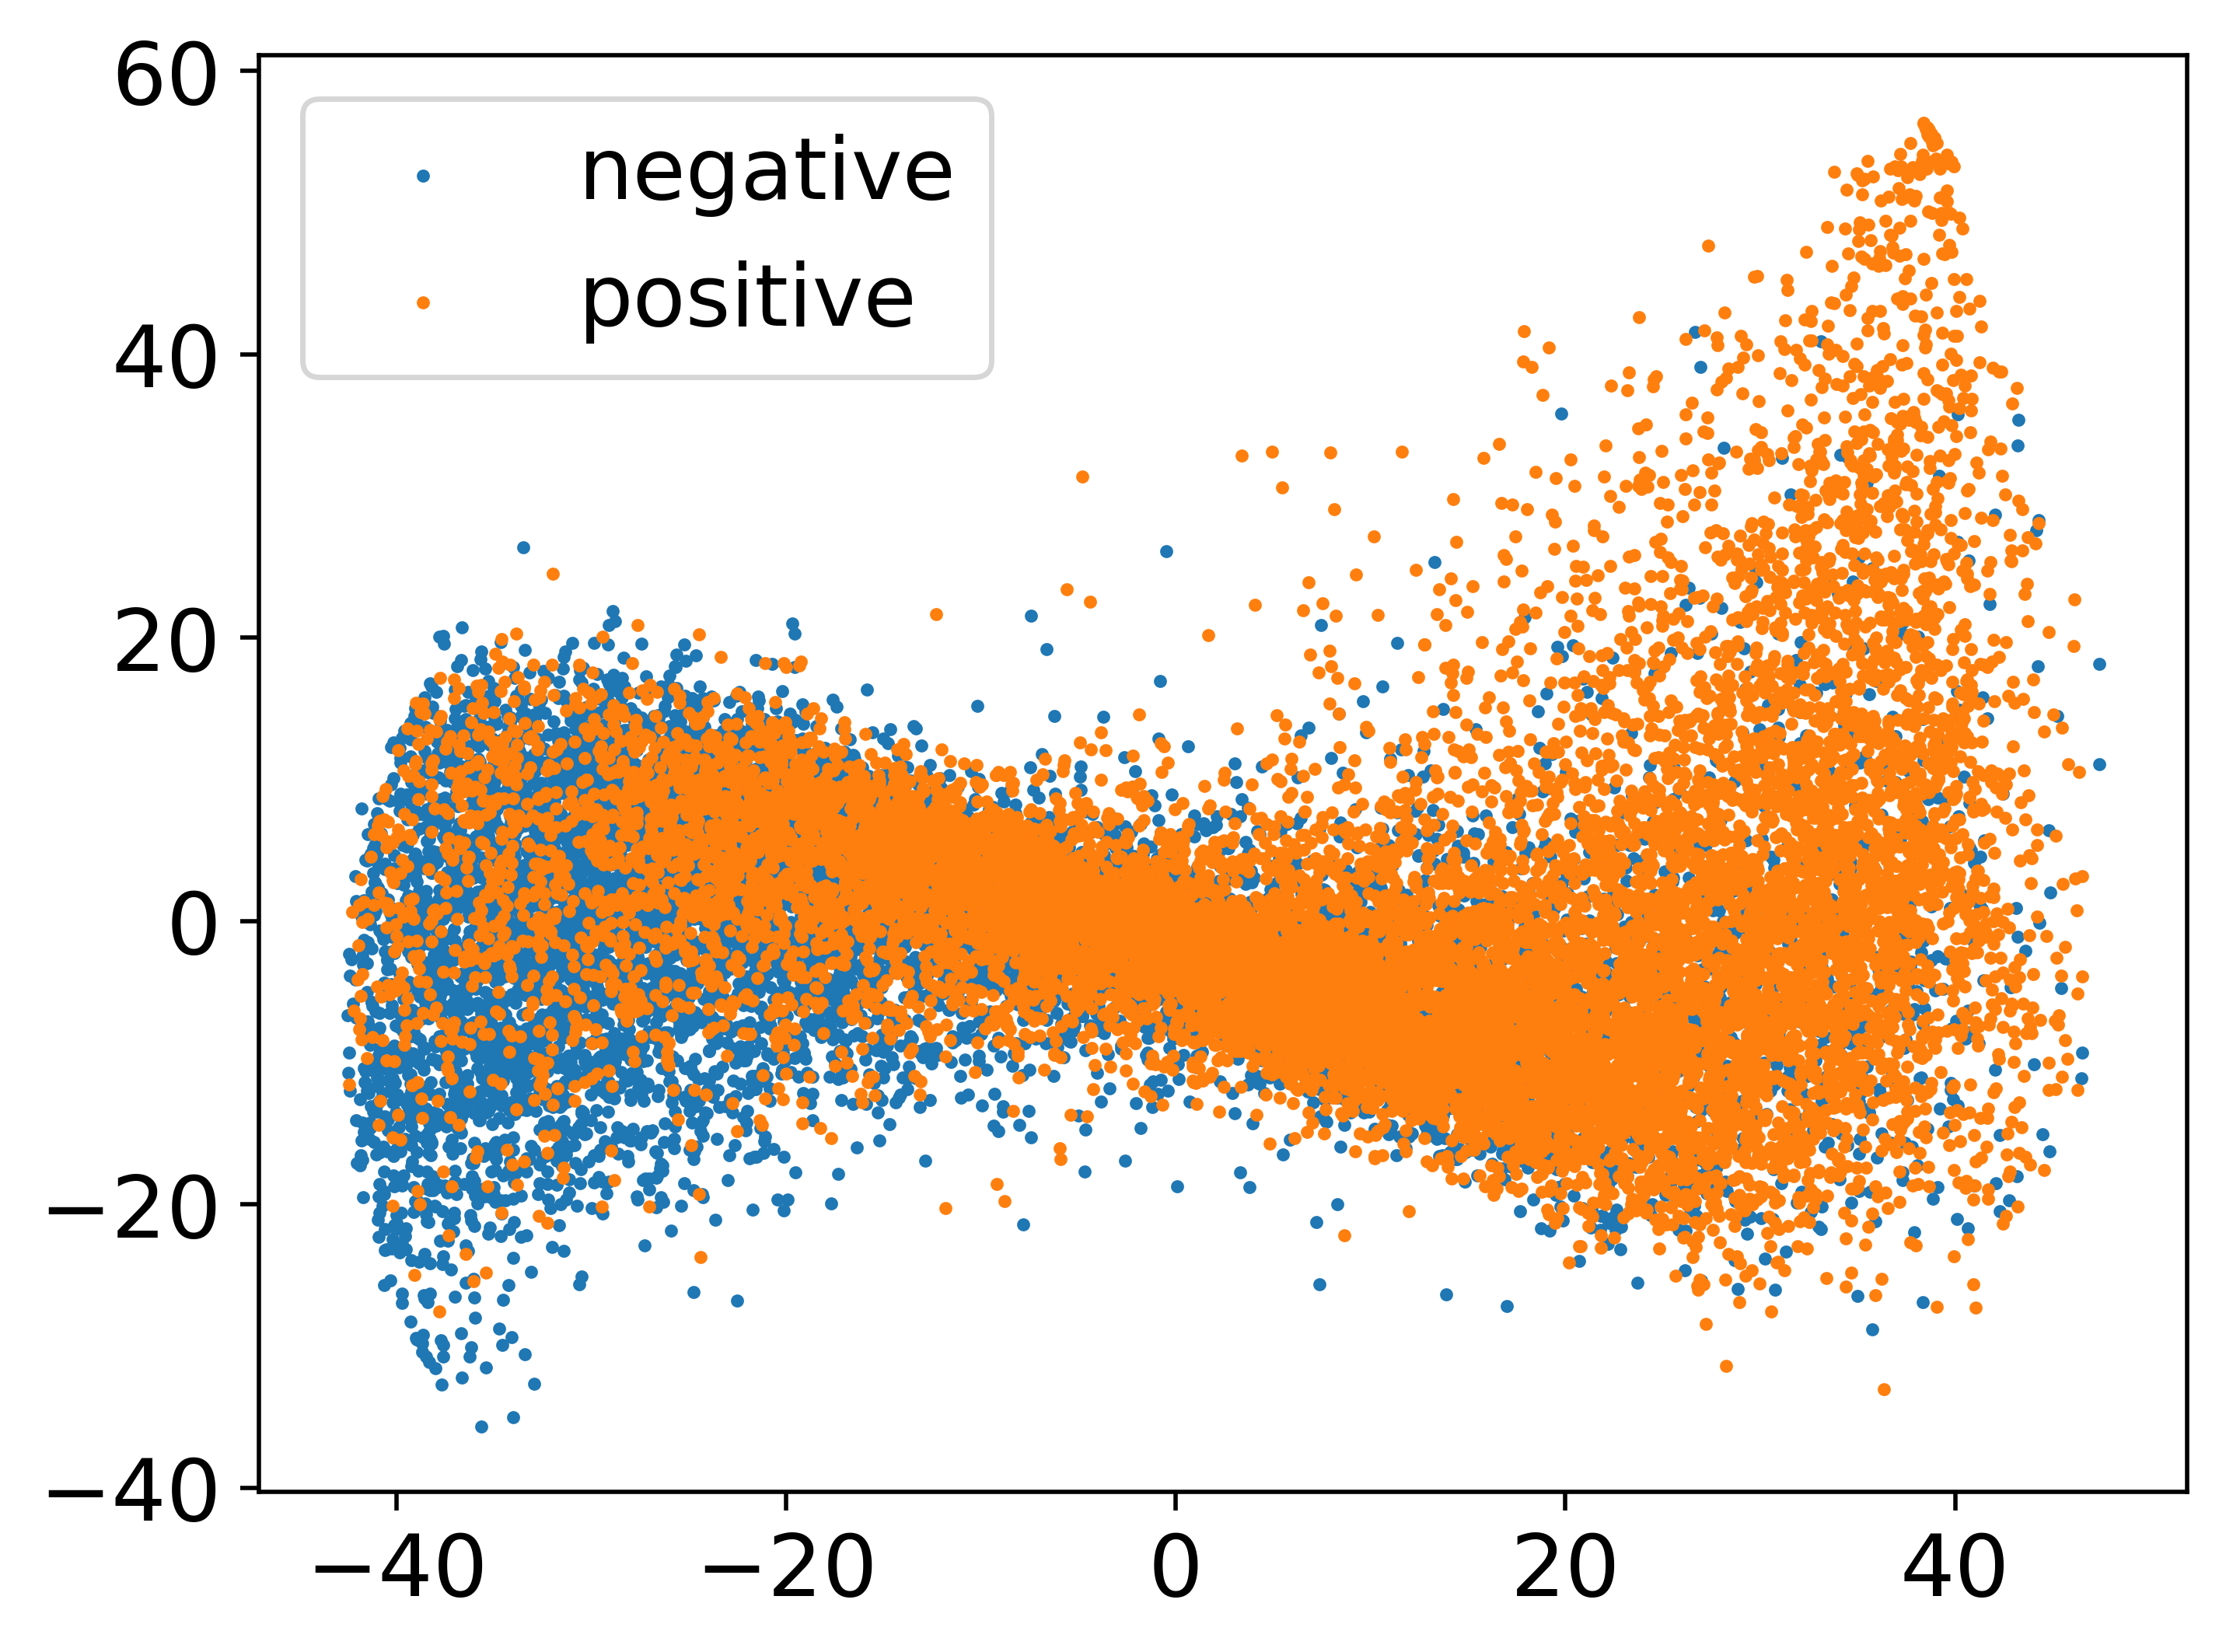
\includegraphics[width=\textwidth]{figures/pca_scatter_document_level.png}
        \caption{Each point represents one document after averaging the sequence embeddings.}
        \label{figure:pca_document}
    \end{subfigure}
    \caption{Dimension reduced plots of the datapoints with \ac{PCA}.}
    \label{figure:pca}
\end{figure}

\subsection{K-nearest neighbor classifier}
As a second classifier the K-nearest neighbor classifier was tested.
Similar to the Naive Bayes classifier, the sequence embeddings were averaged per report.
To determine the value of K, the validation curve in Figure \ref{figure:knn_validation} was created with 5-fold cross-validation, which shows the classification accuracy for uneven values of k in the range of 3 to 350.
\begin{figure}[h]
    \centering
    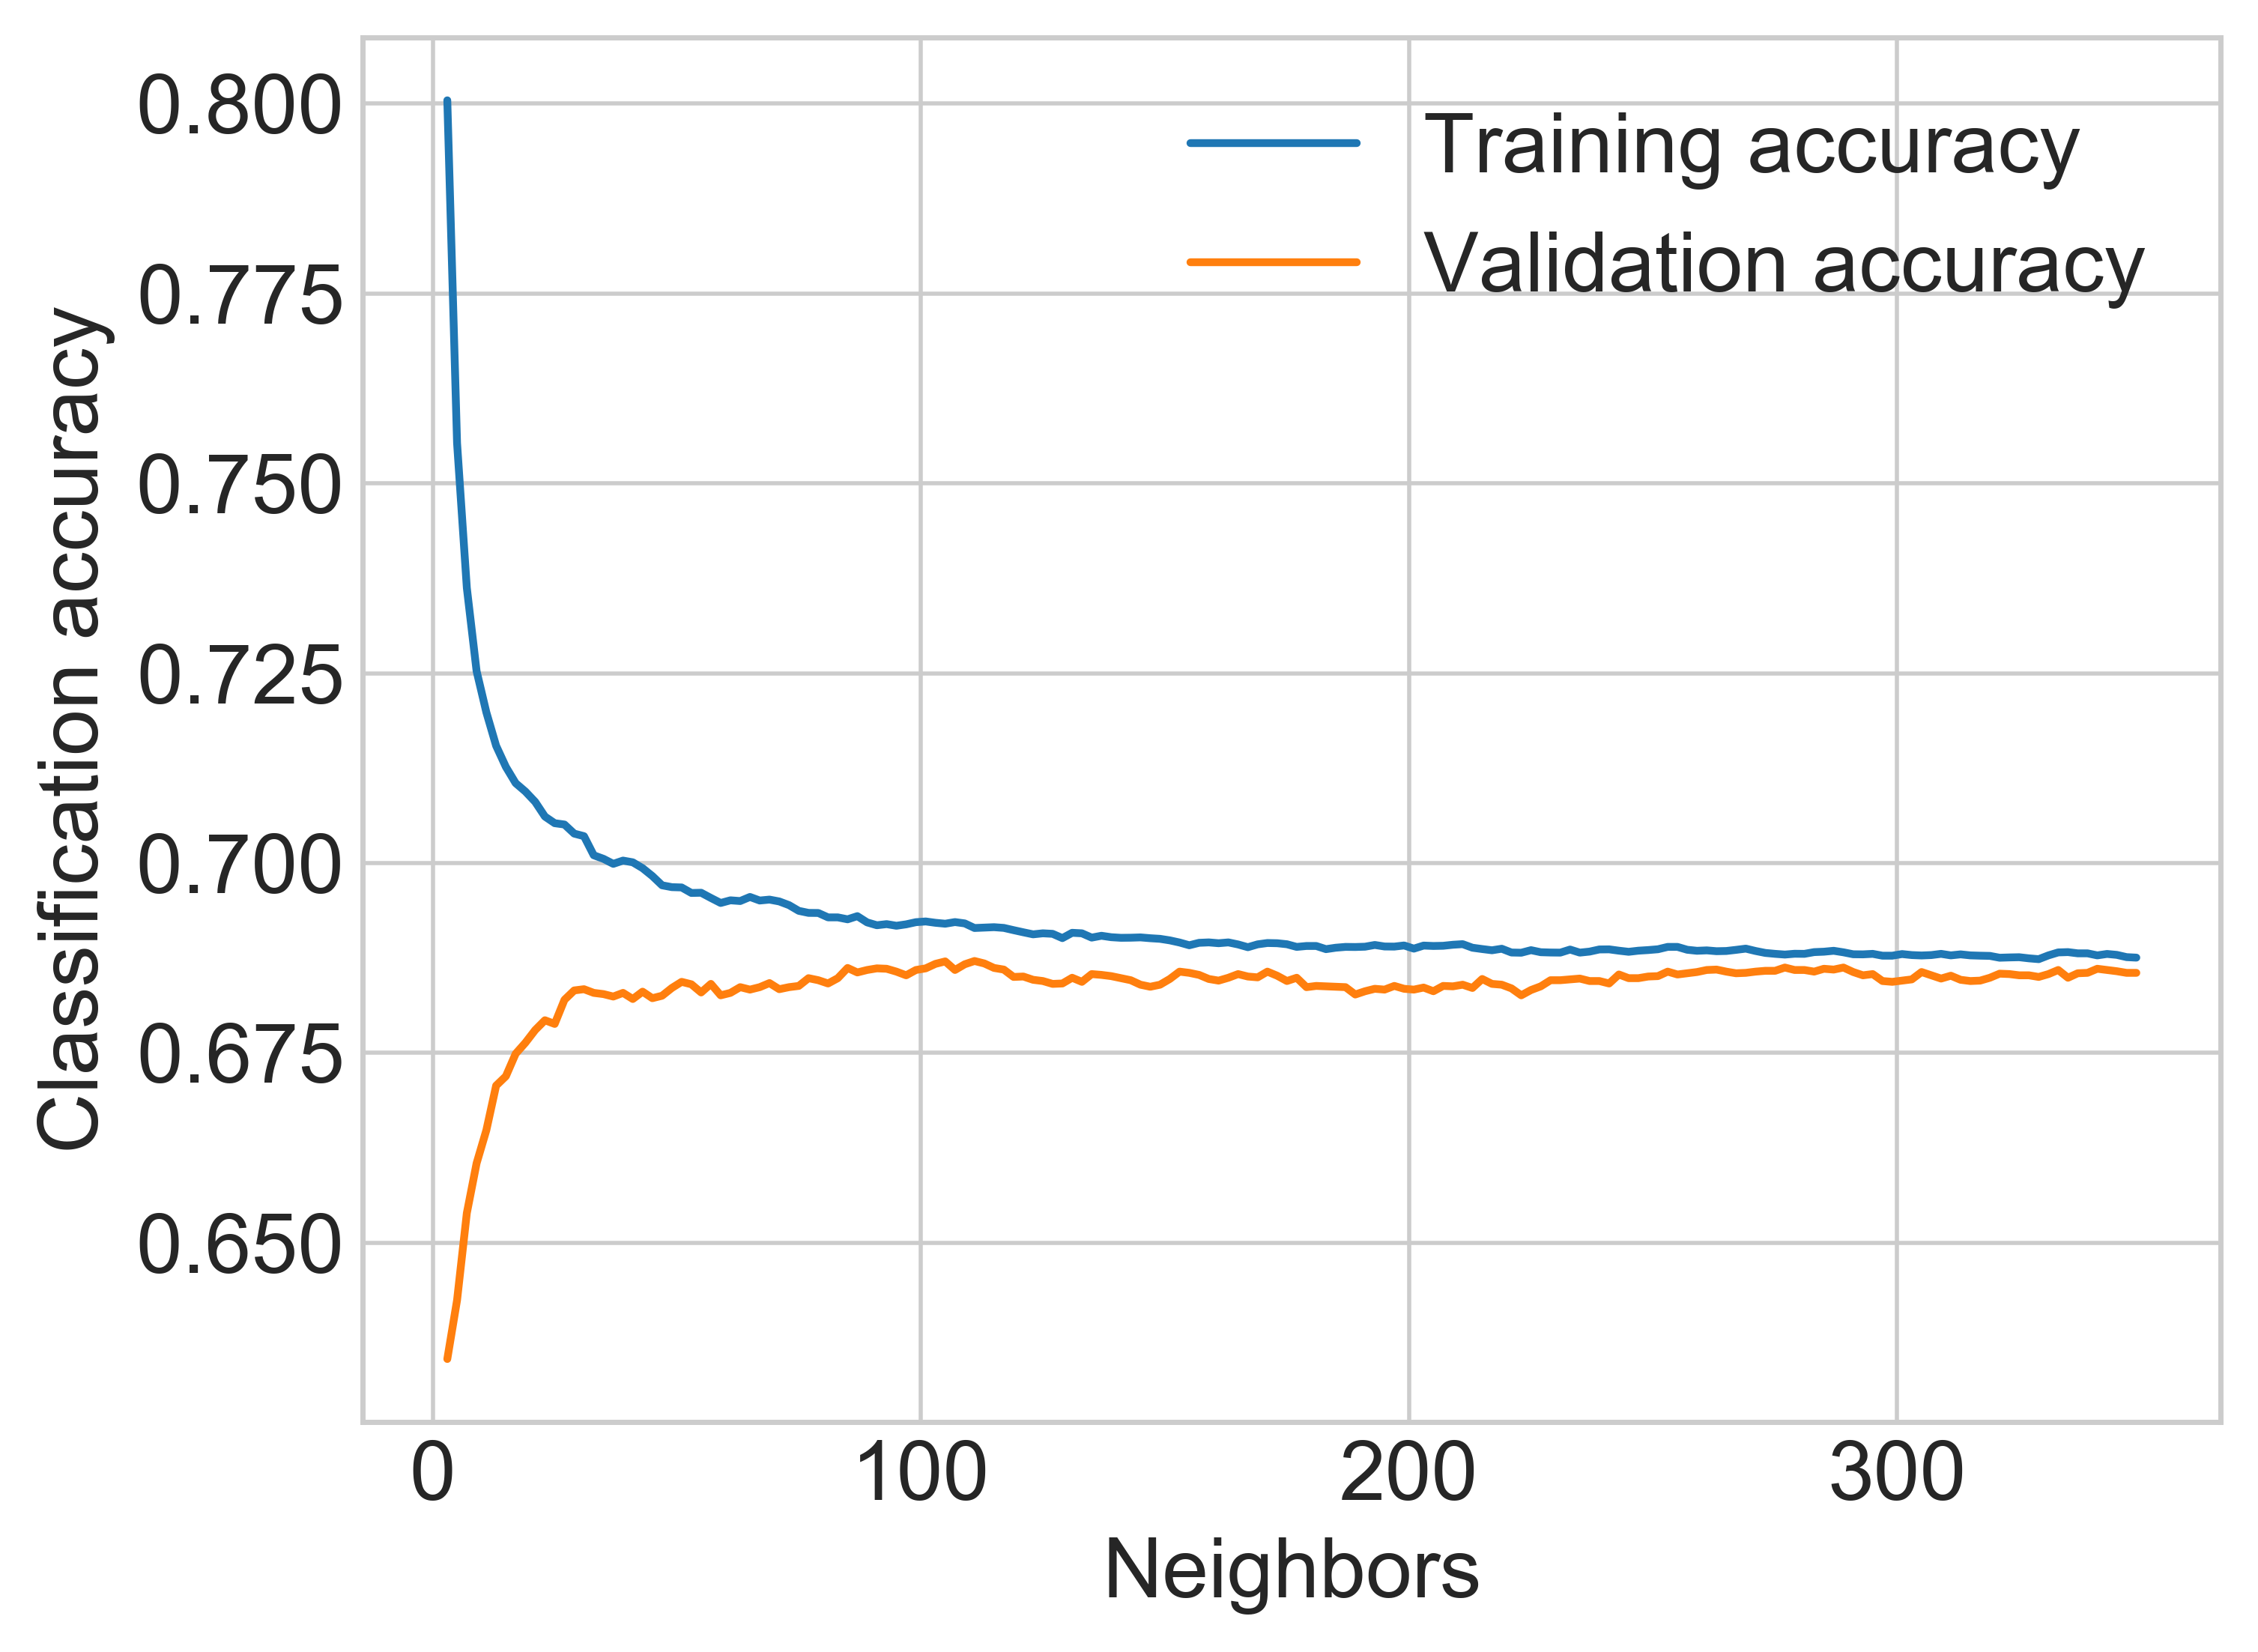
\includegraphics[width=0.5\textwidth]{figures/charts/knn_validation.png}
    \caption{Validation curve for the K-nearest neighbor classifier.}
    \label{figure:knn_validation}
\end{figure}
The highest score is reached for $K=111$ neighbors with a validation accuracy of 68.7\%.
Setting \textit{K} to 111 leads to the learning curve in figure \ref{figure:knn_learning}.
\begin{figure}[h]
    \centering
    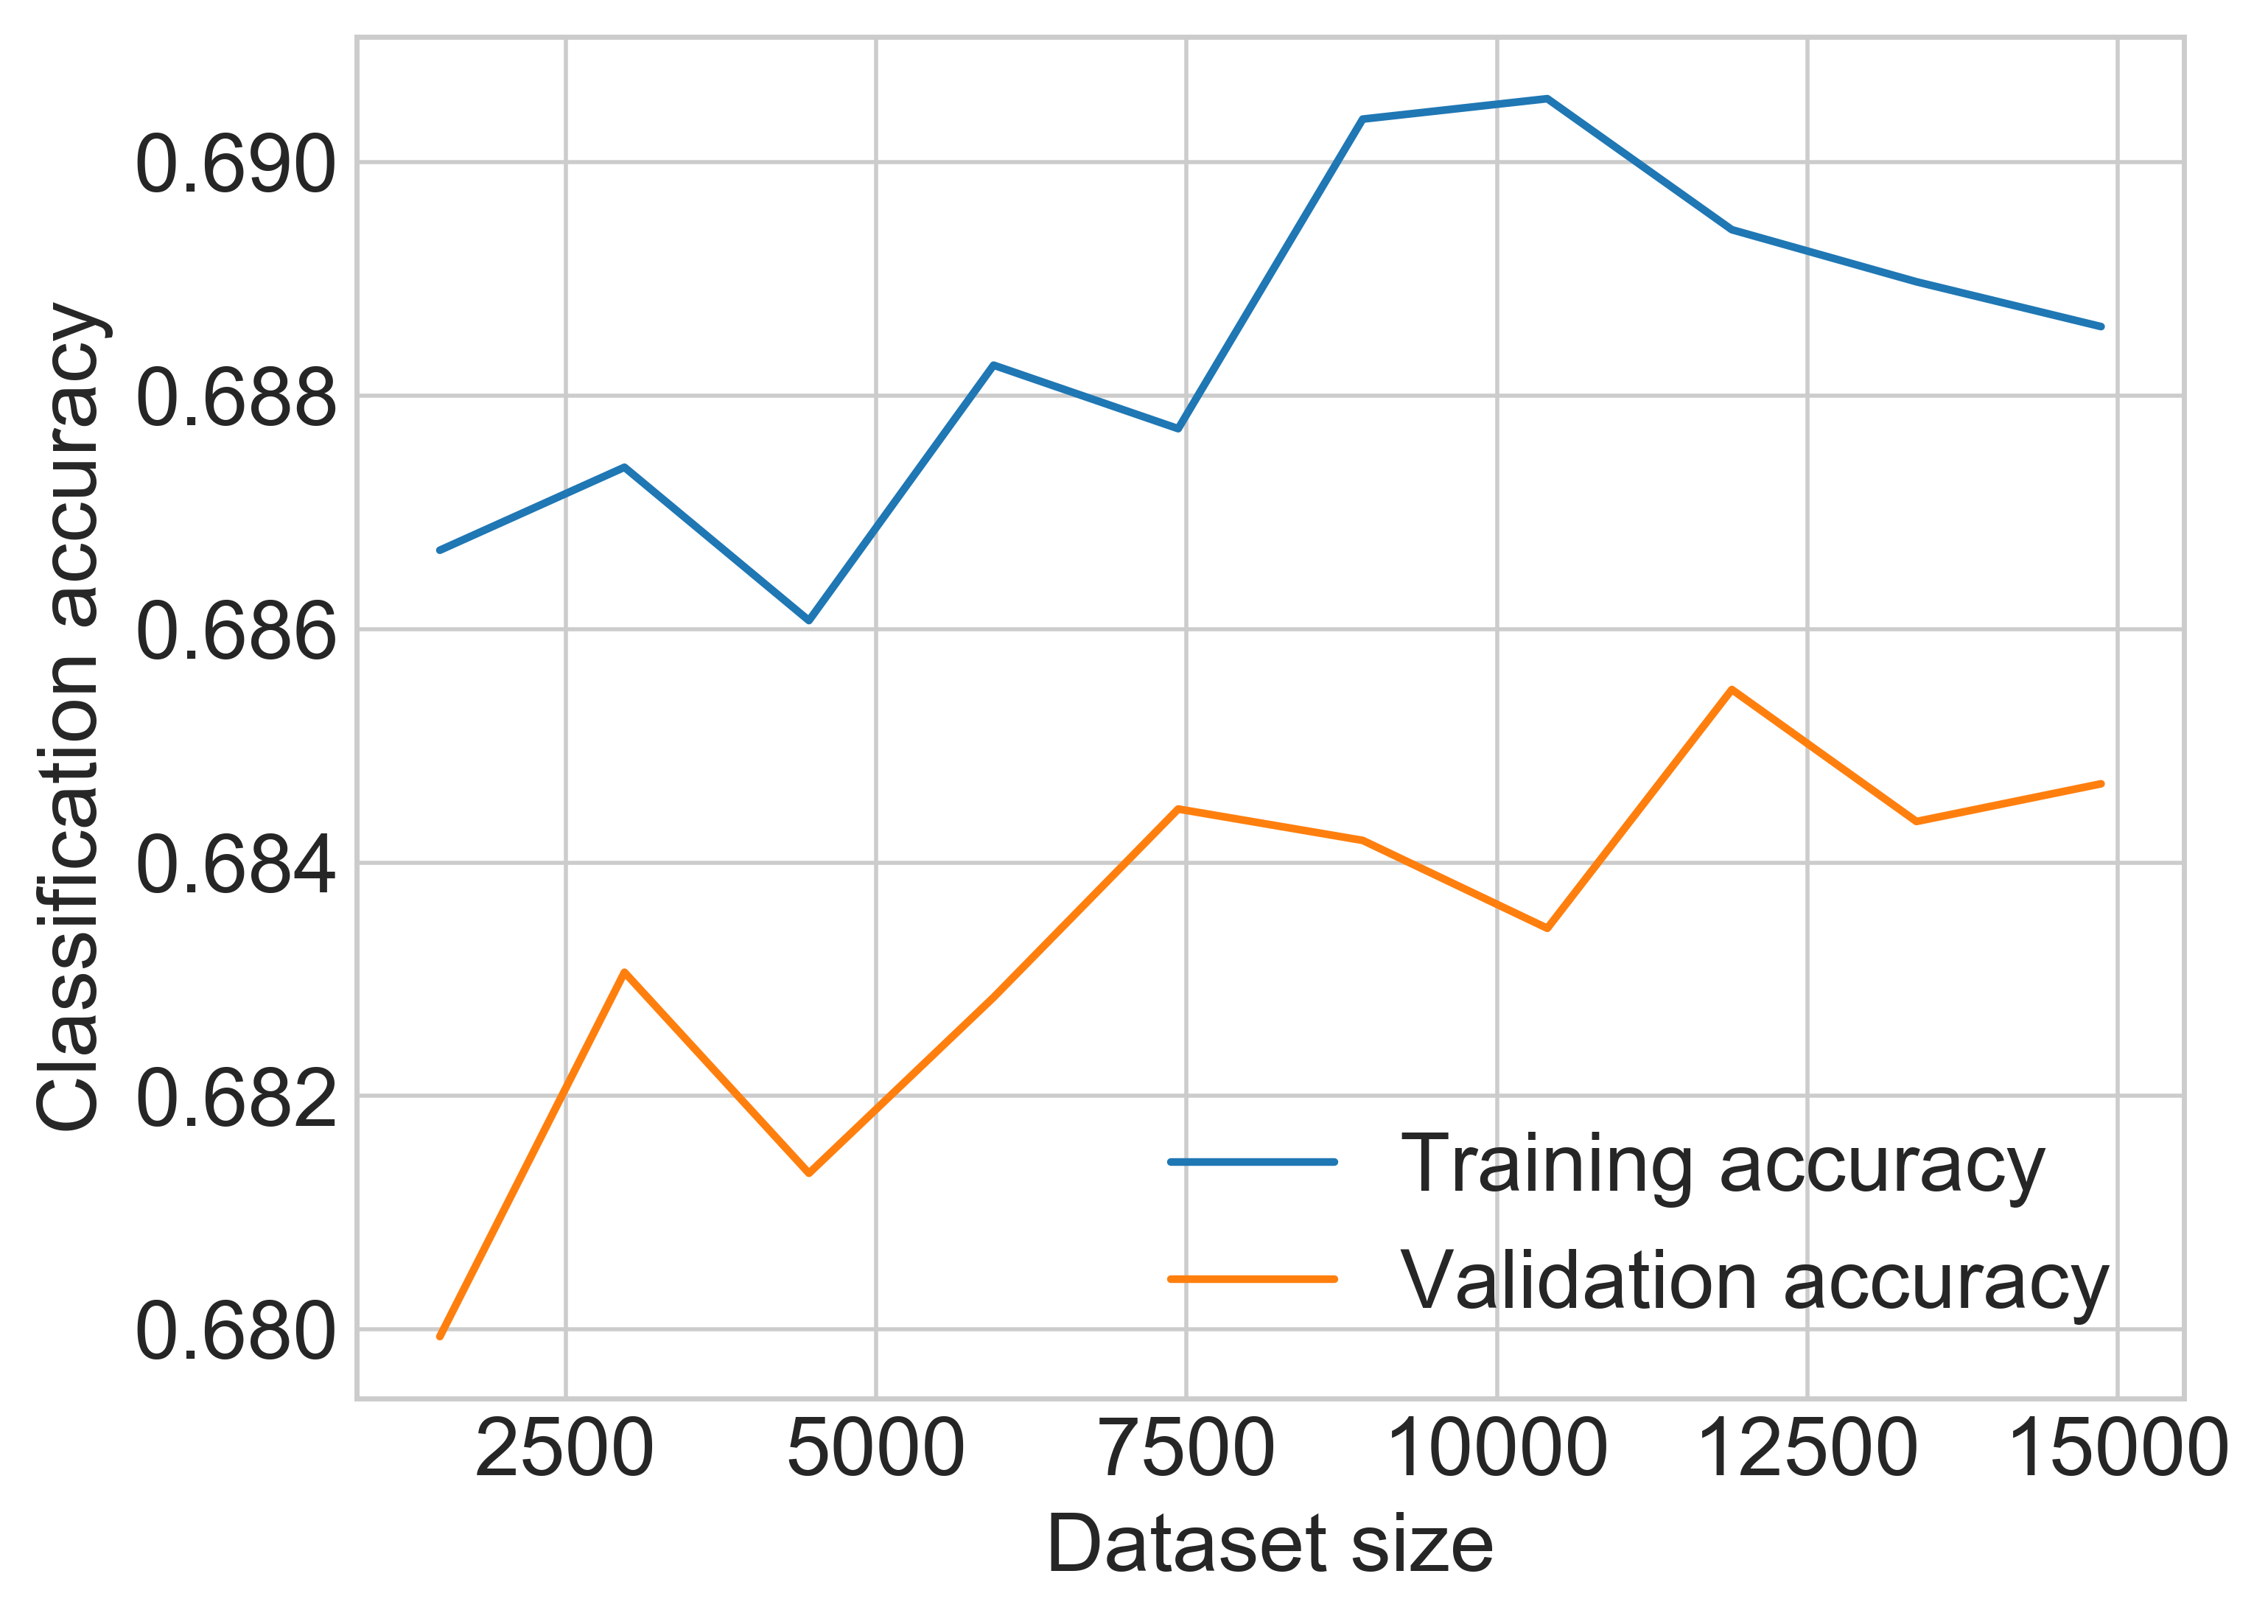
\includegraphics[width=0.5\textwidth]{figures/charts/knn_learning.png}
    \caption{Learning curve for the K-nearest neighbor classifier with K=111.}
    \label{figure:knn_learning}
\end{figure}
The learning curve shows that the model benefits from using many training samples and might improve even more, when more data is provided.
For $K=111$ an accuracy of 68.3\% was reached on an independent test dataset.

\subsection{\acl{SVM}}
Finally also the predictive ability of the \ac{SVM} was examined.
Again the sequence embeddings were averaged per report.
A full grid search over different hyperparameters to find the best solution did not finish in acceptable time and was aborted after four days running.
A manual test run indicated, that this might be because of the linear kernel, which did not finish training in this test run.
Figure \ref{figure:svm_validation} shows the validation curves for C values of 100, 1000, 10000 and 100000.
Each run was done with the \textit{rbf} kernel and gamma values of $\gamma=10^{-7}$, $10^{-6}$, $10^{-5}$, $10^{-4}$, $0.001$, $0.01$, $0.1$, $1$, $10$, $100$.
\begin{figure}[h]
    % \begin{subfigure}{0.5\textwidth}
    %     \centering
    %     \includegraphics[width=\textwidth]{figures/charts/svm_validation_C_001.png}
    %     \caption{C=0.01}
    %     \label{figure:svm_validation_C_001}
    % \end{subfigure}
    % \begin{subfigure}{0.5\textwidth}
    %     \centering
    %     \includegraphics[width=\textwidth]{figures/charts/svm_validation_C_01.png}
    %     \caption{C=0.1}
    %     \label{figure:svm_validation_C_01}
    % \end{subfigure}
    \begin{subfigure}{0.5\textwidth}
        \centering
        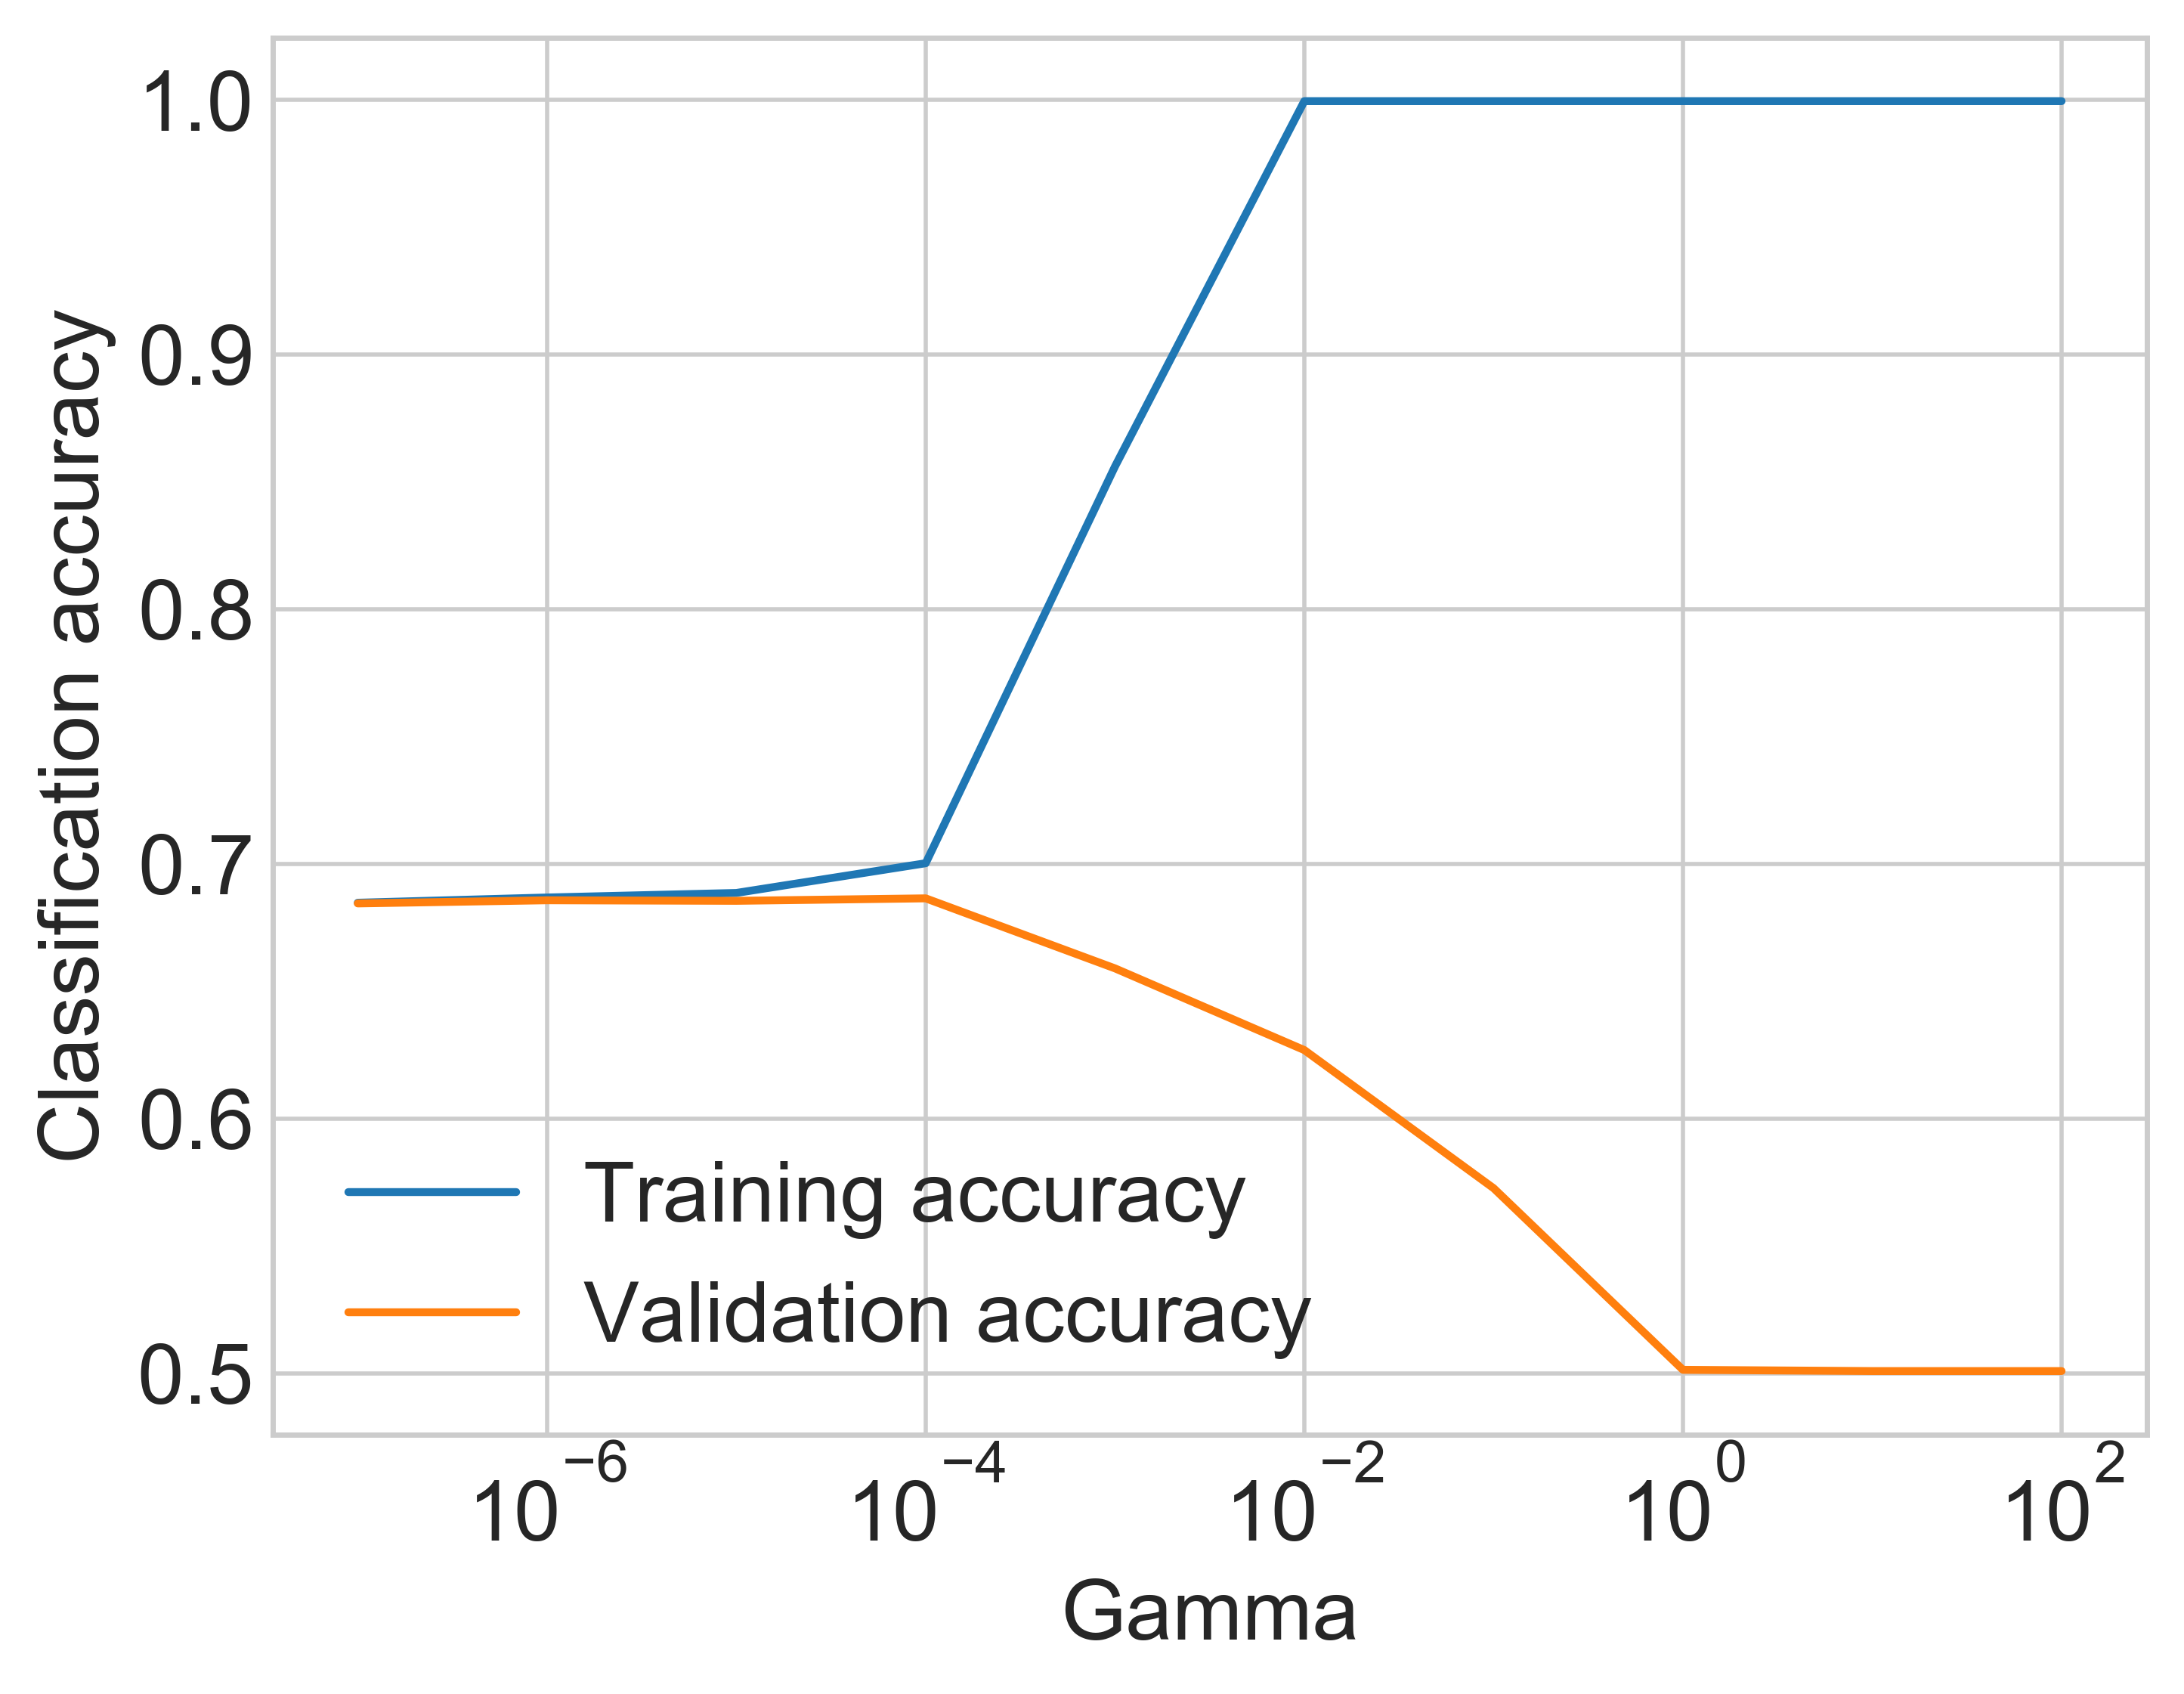
\includegraphics[width=\textwidth]{figures/charts/svm_validation_C_100.png}
        \caption{C=100}
        \label{figure:svm_validation_C_100}
    \end{subfigure}
    \begin{subfigure}{0.5\textwidth}
        \centering
        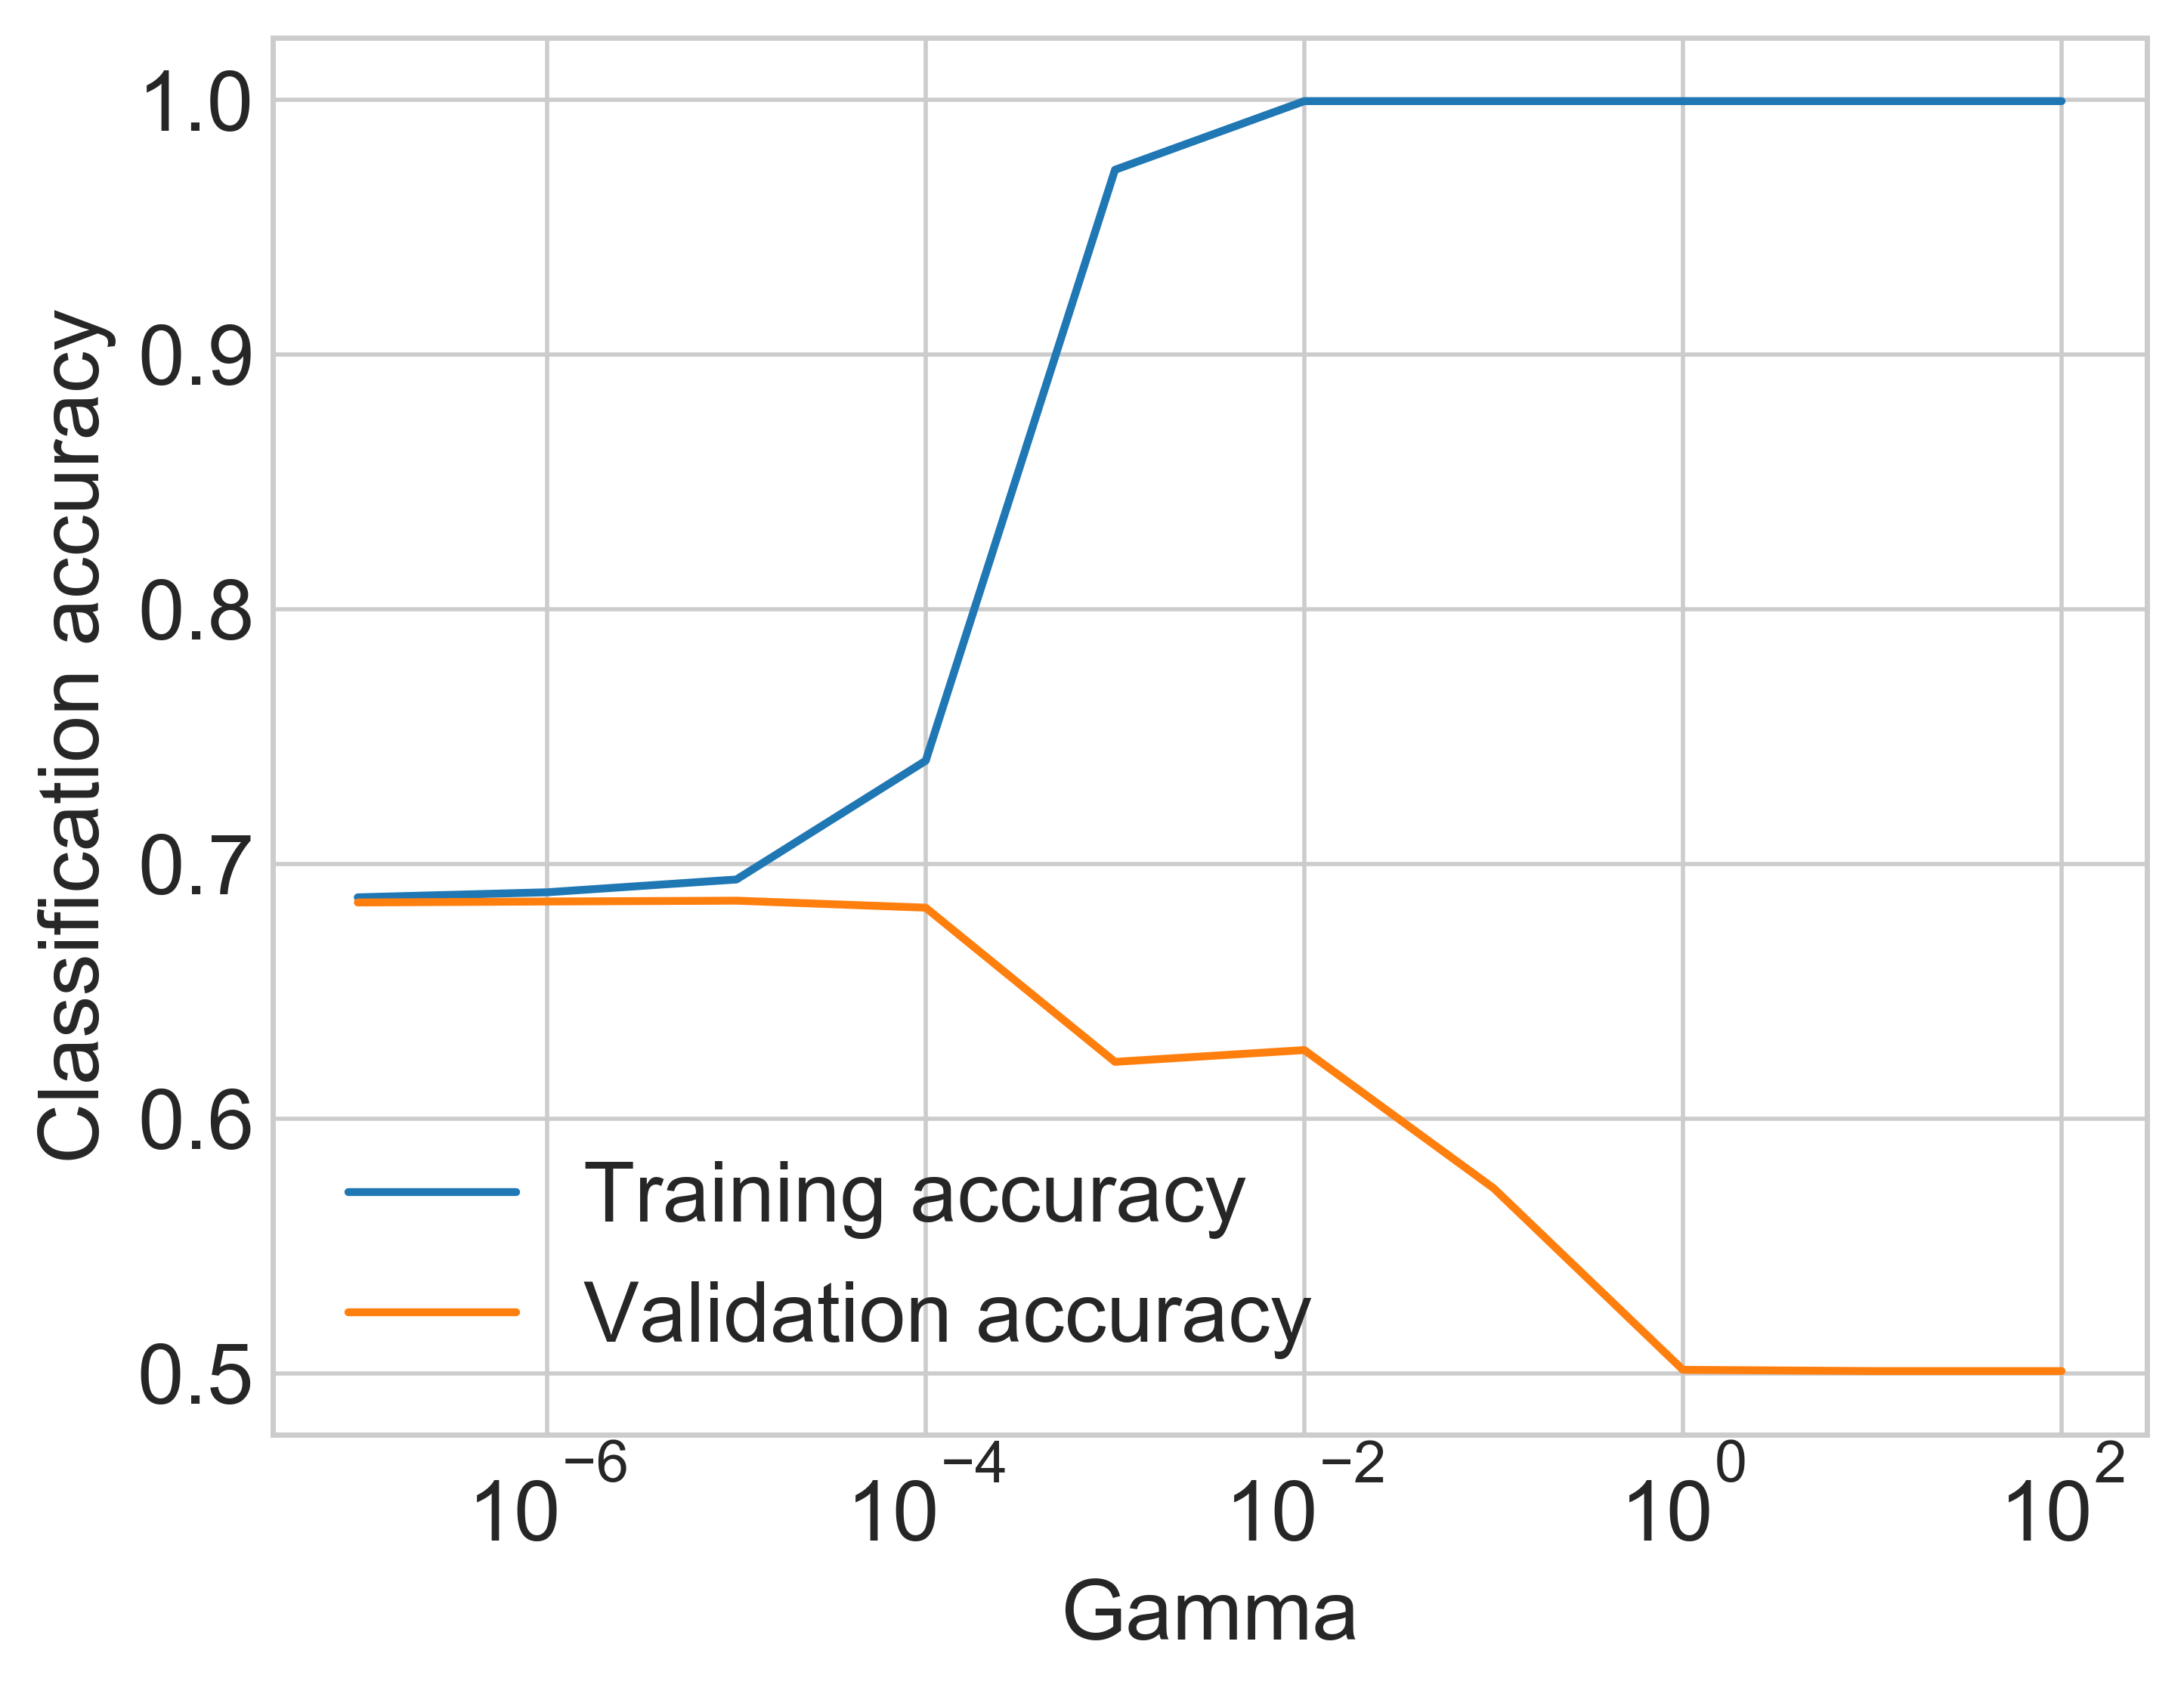
\includegraphics[width=\textwidth]{figures/charts/svm_validation_C_1000.png}
        \caption{C=1000}
        \label{figure:svm_validation_C_1000}
    \end{subfigure}
    \begin{subfigure}{0.5\textwidth}
        \centering
        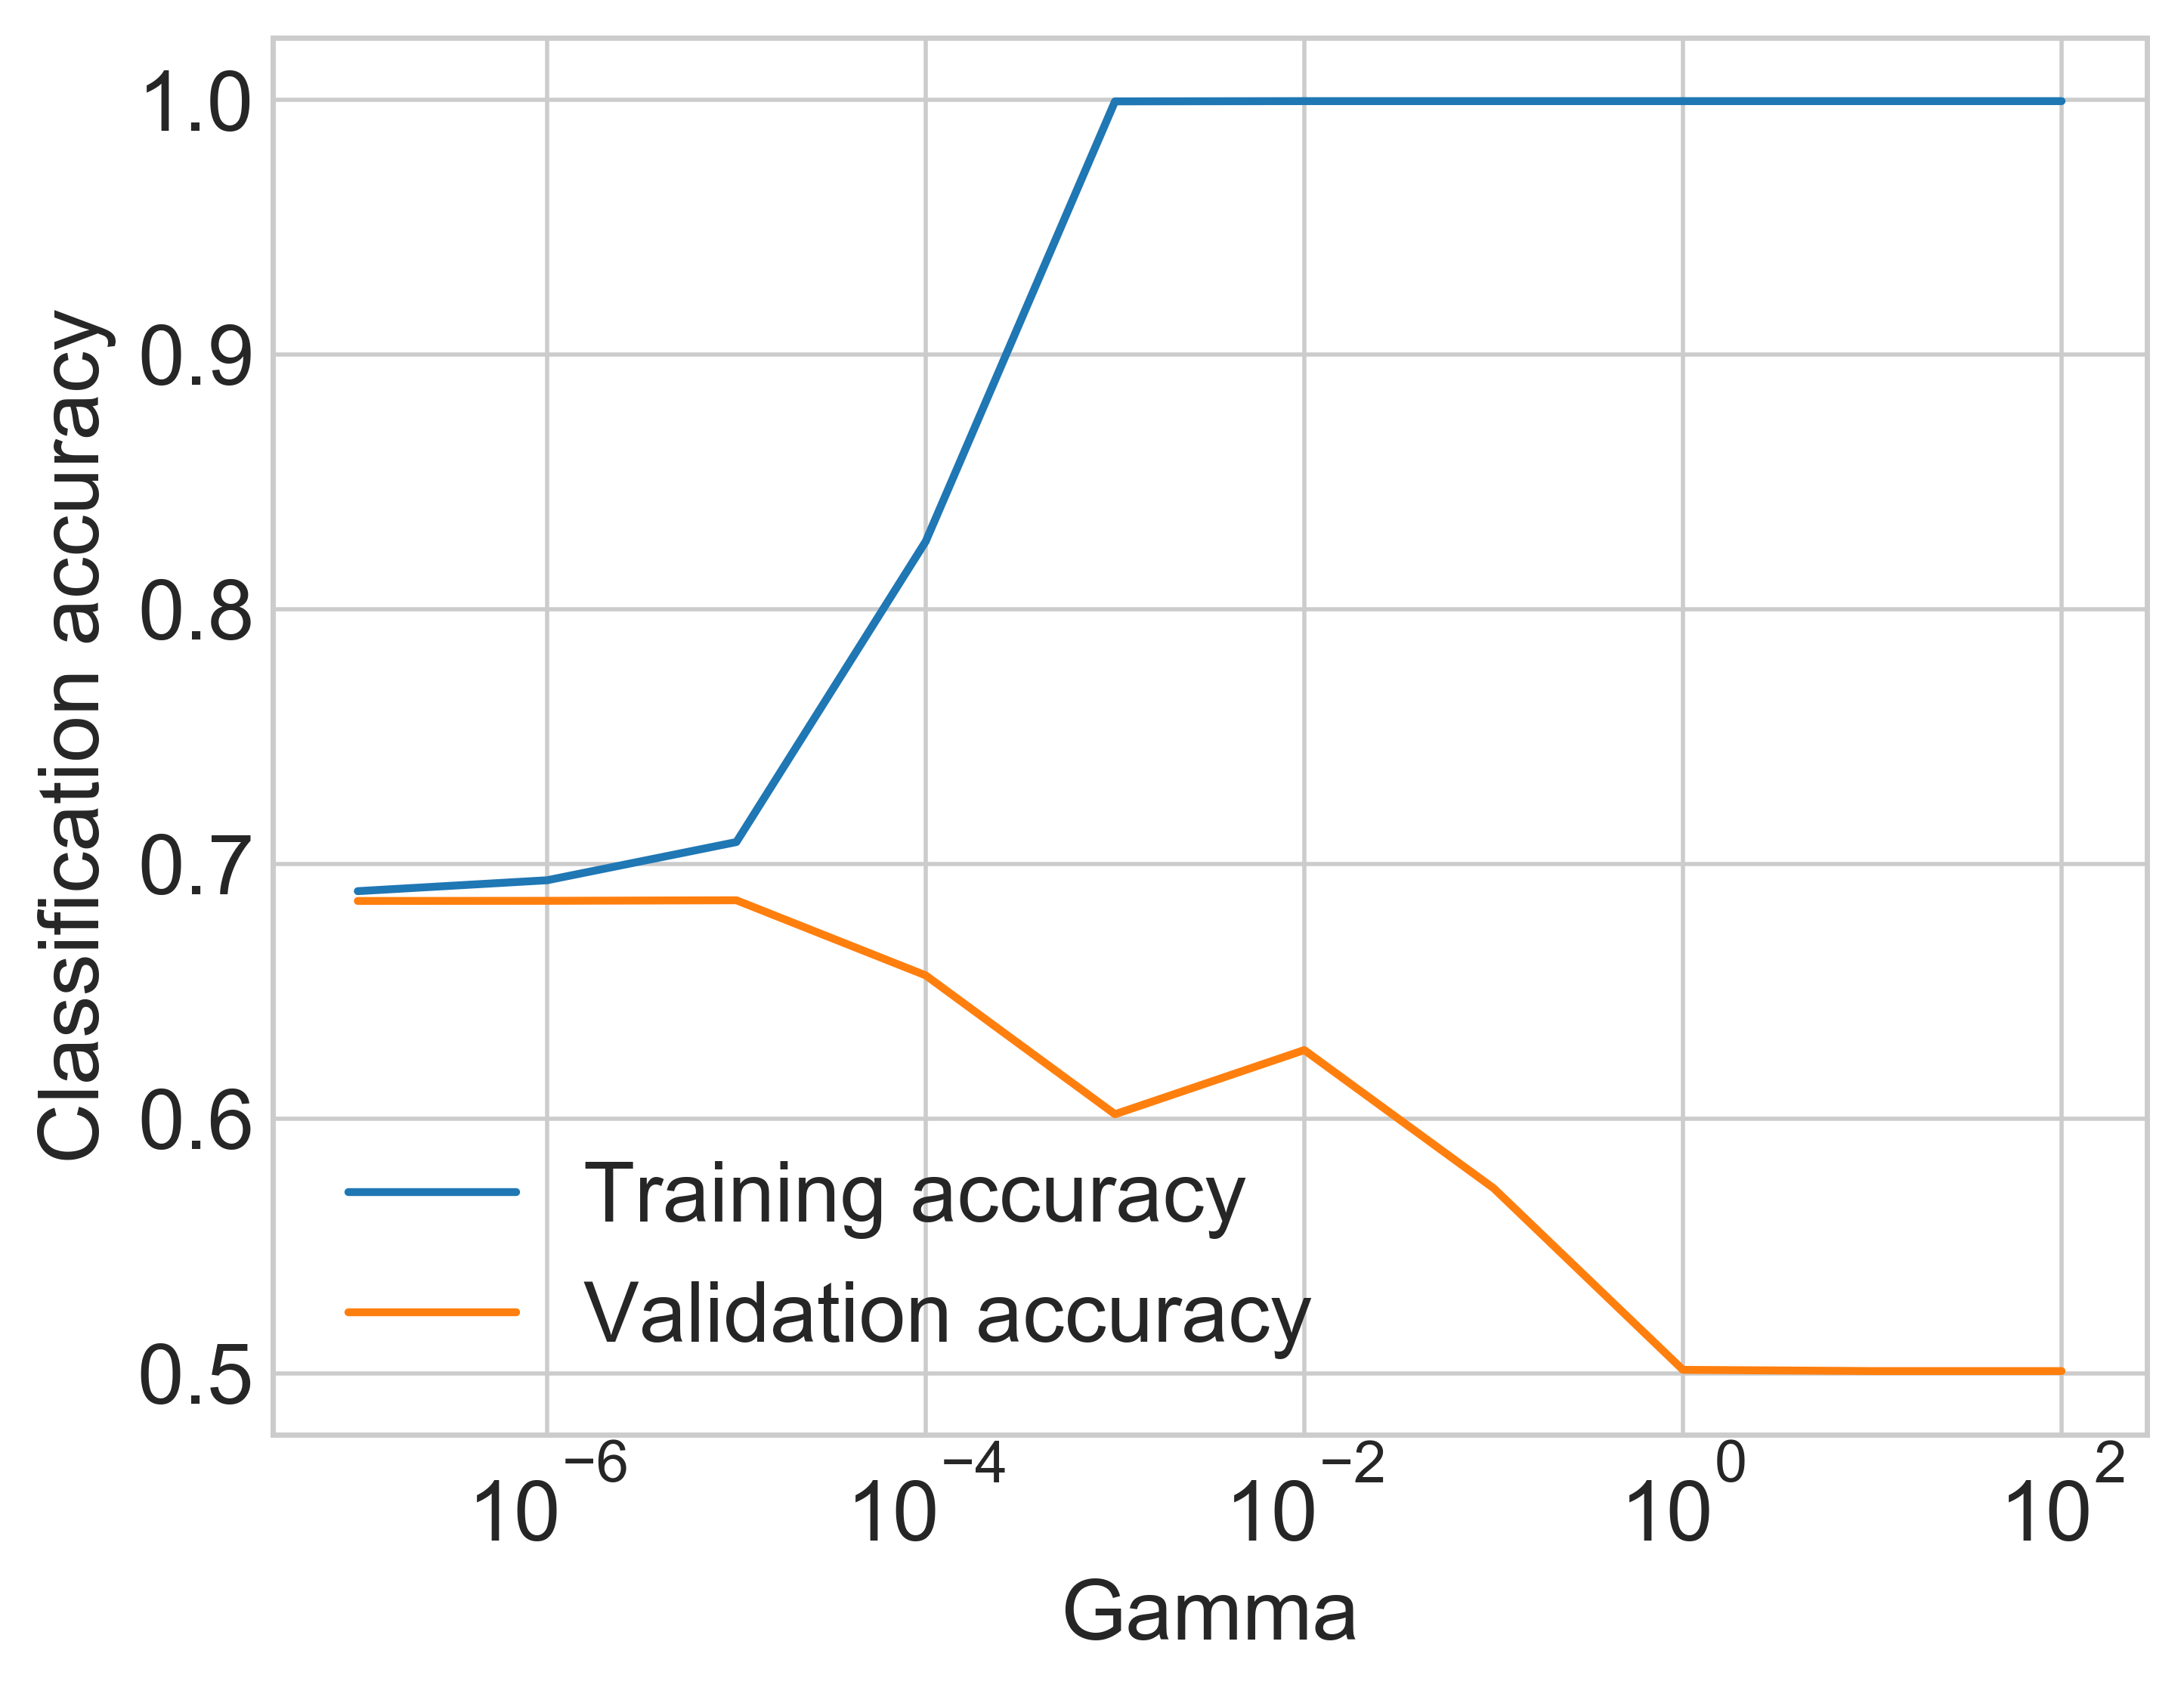
\includegraphics[width=\textwidth]{figures/charts/svm_validation_C_10000.png}
        \caption{C=10000}
        \label{figure:svm_validation_C_10000}
    \end{subfigure}
    \begin{subfigure}{0.5\textwidth}
        \centering
        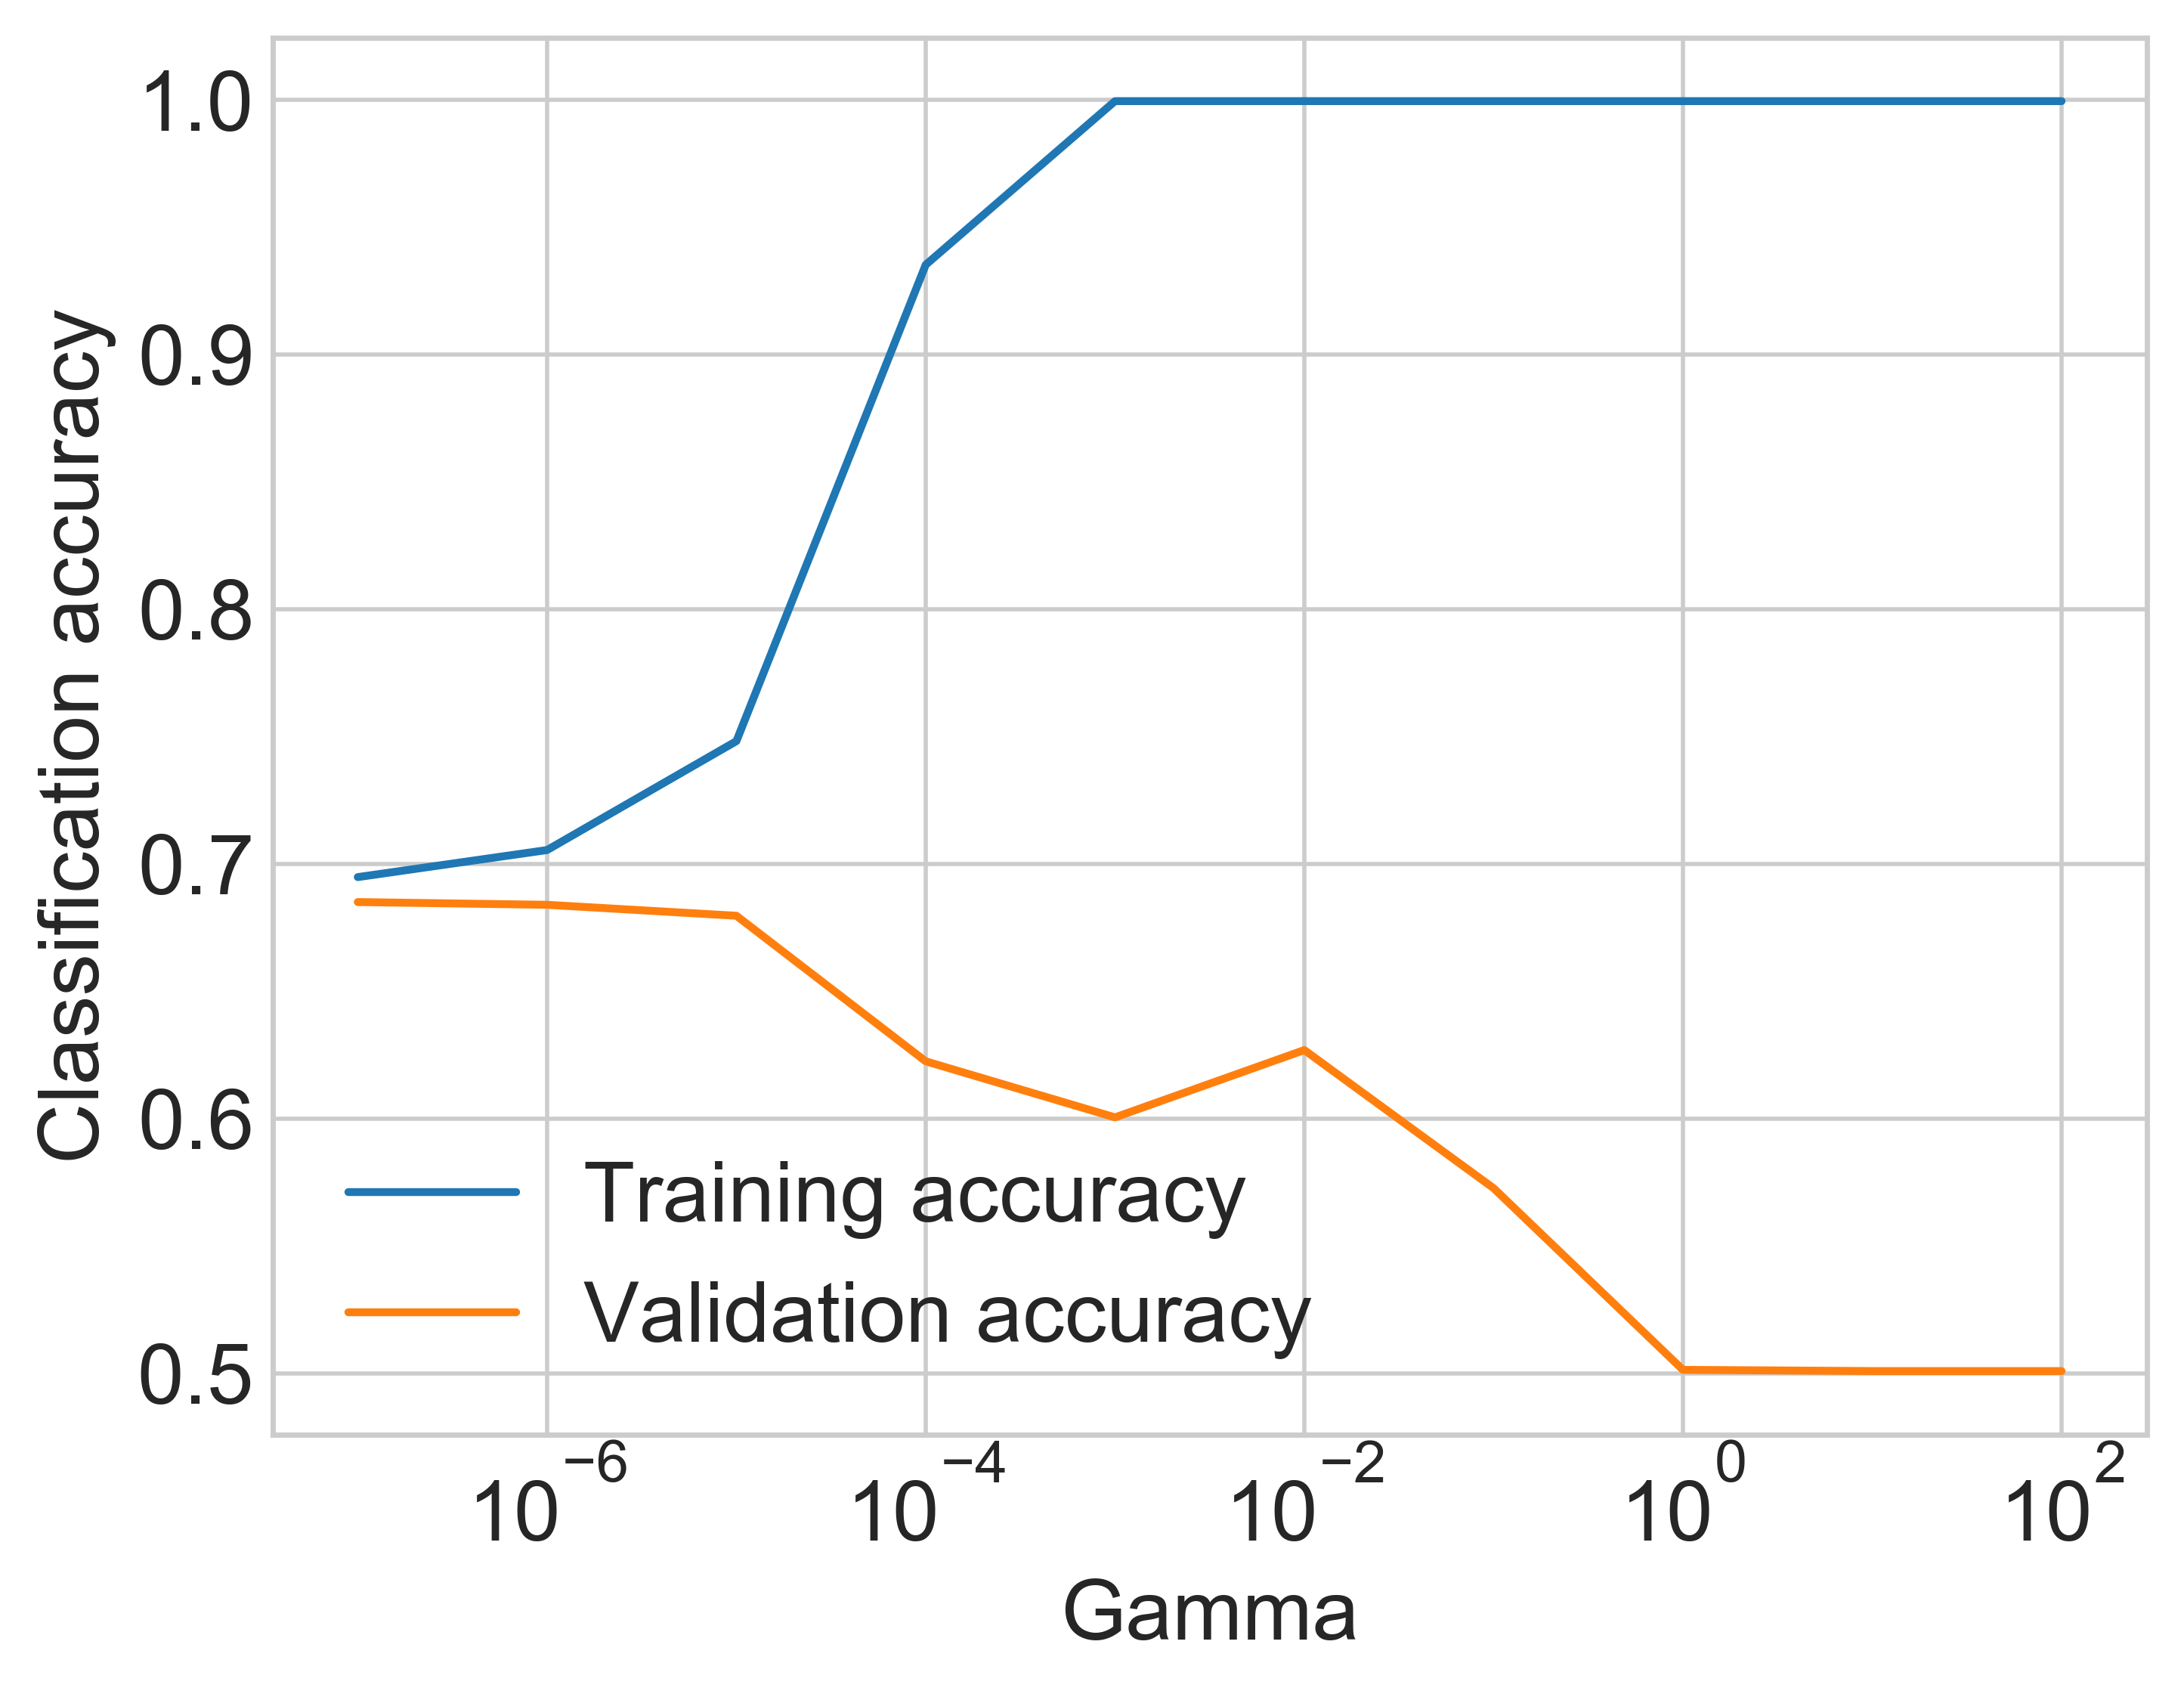
\includegraphics[width=\textwidth]{figures/charts/svm_validation_C_100000.png}
        \caption{C=100000}
        \label{figure:svm_validation_C_100000}
    \end{subfigure}
    \caption{Validation curves for different values of C}
    \label{figure:svm_validation}
\end{figure}
The highest score is reached at $C=100$ and $\gamma=0.0001$ with a validation accuracy of 68.7\%.
Using these parameters the learning curve in figure \ref{figure:svm_learning} results.
\begin{figure}[h]
    \centering
    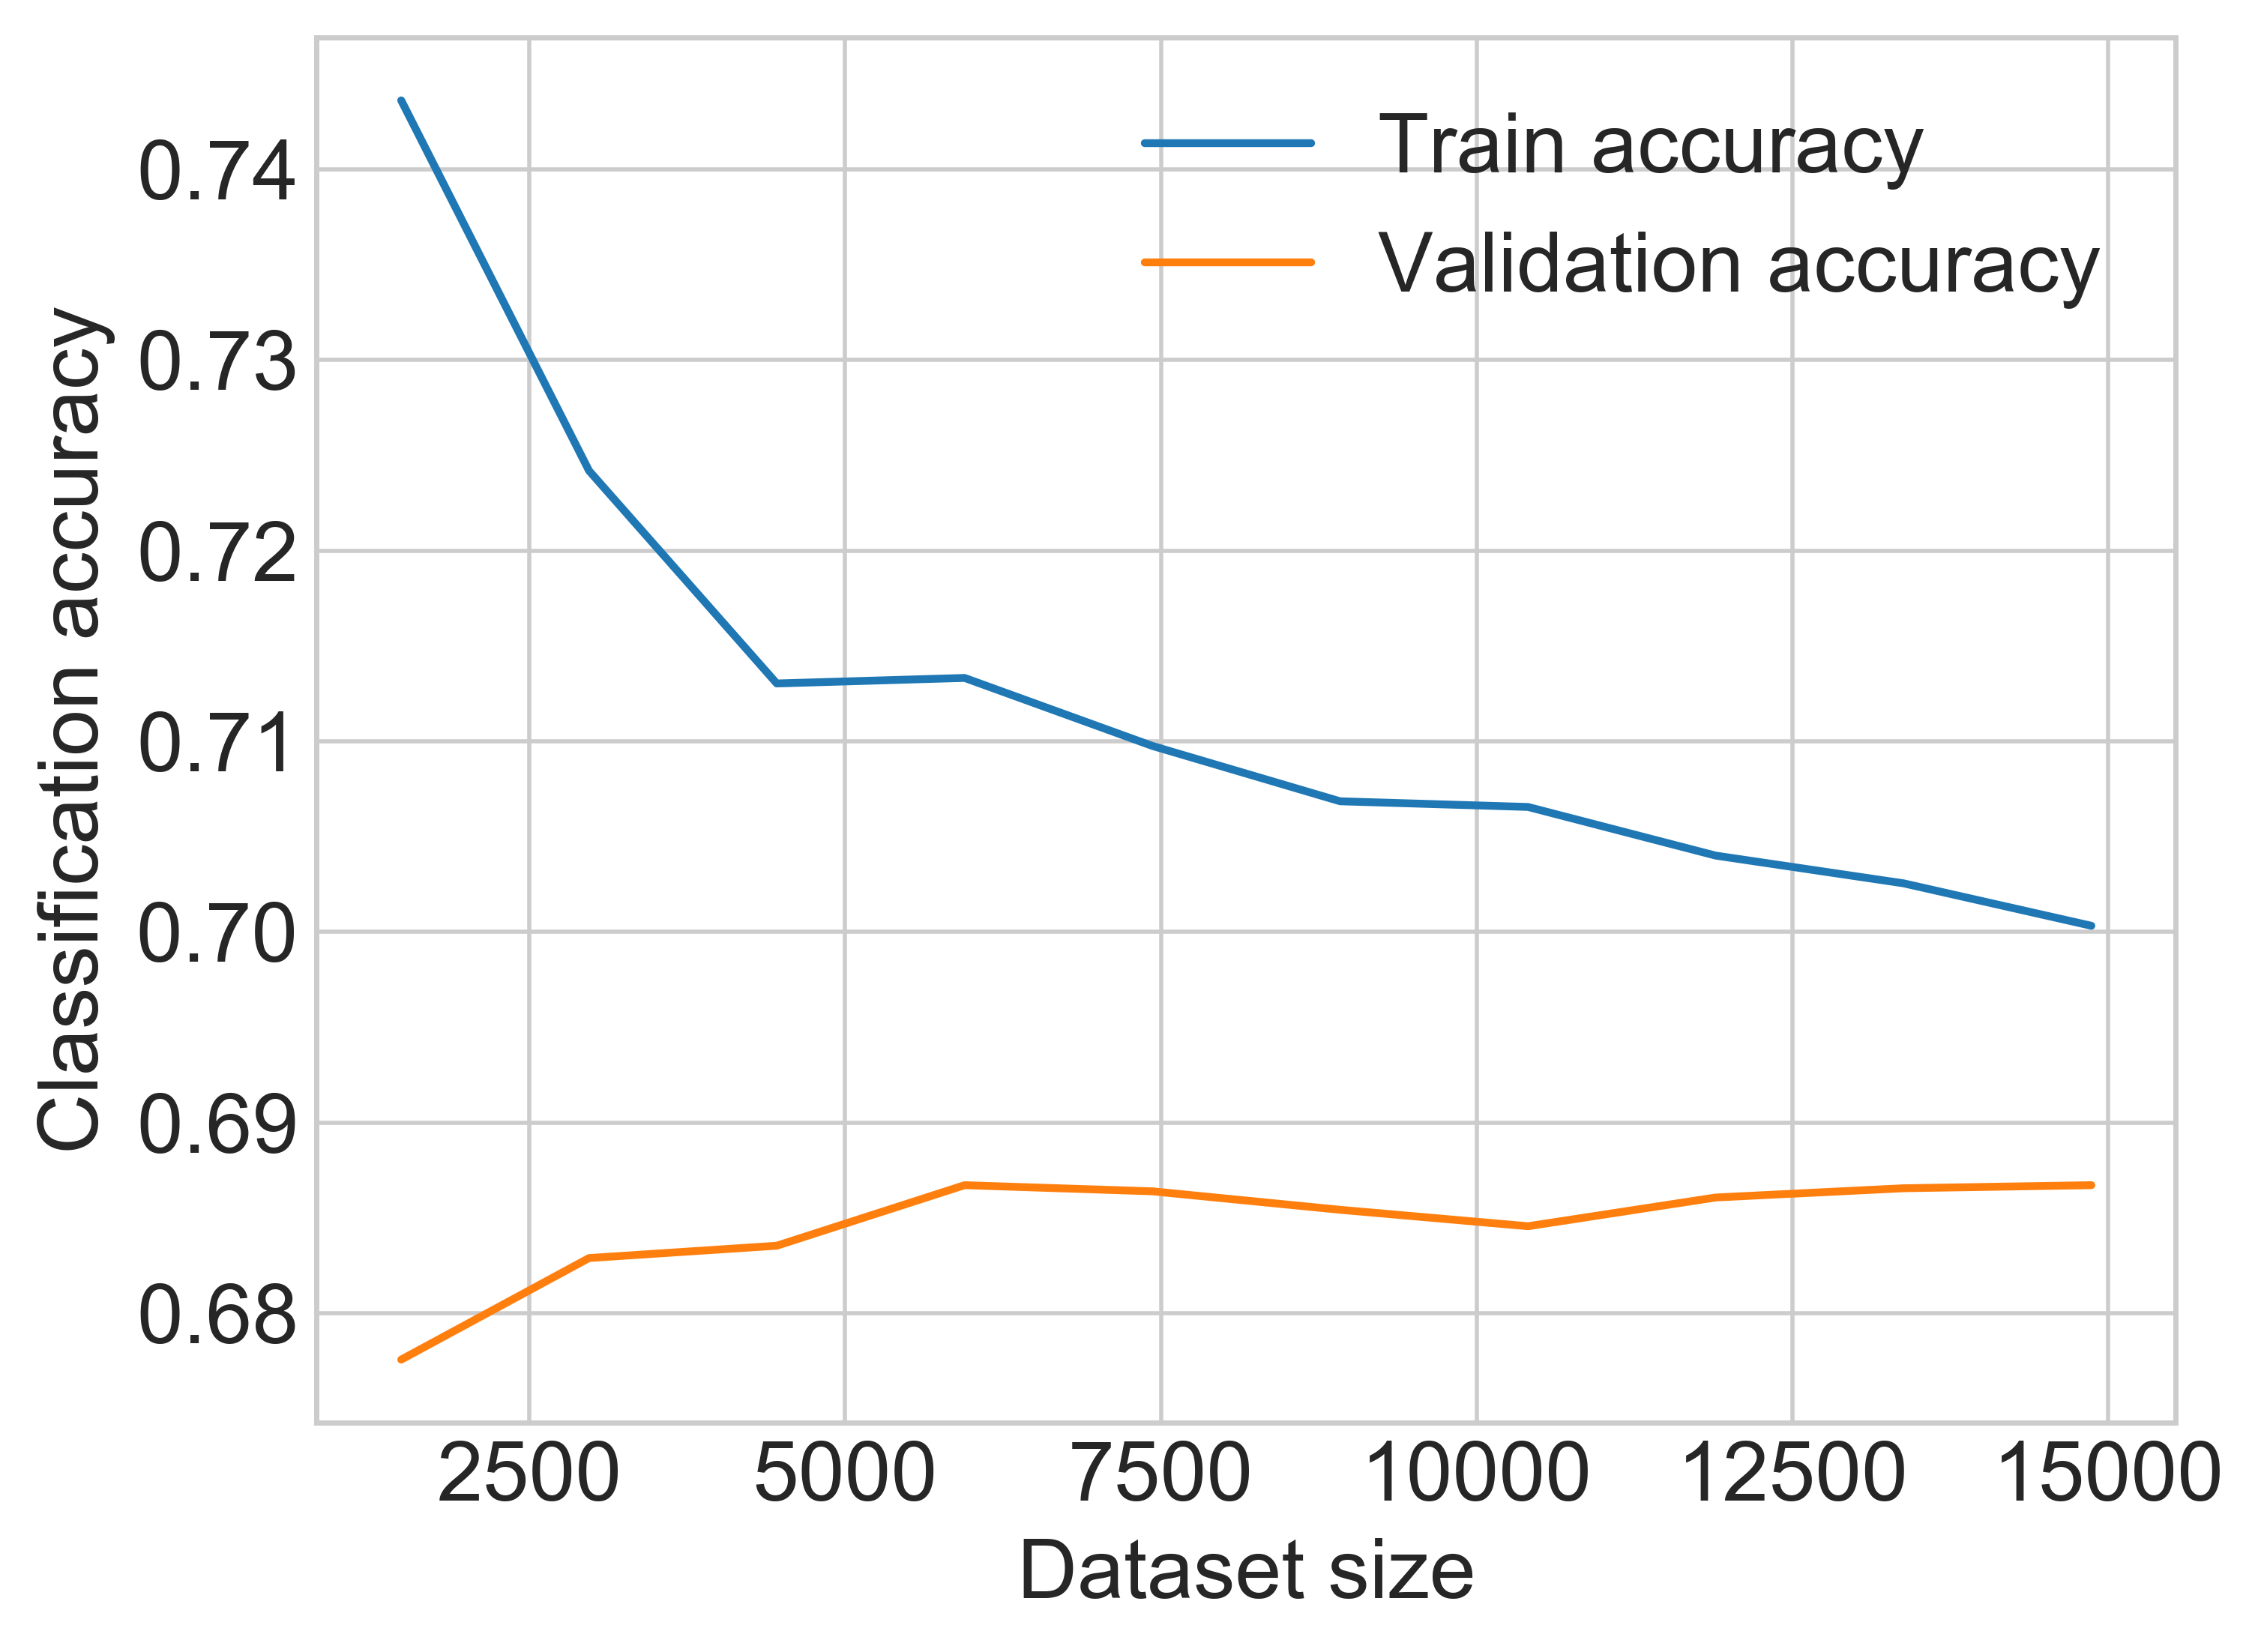
\includegraphics[width=0.5\textwidth]{figures/charts/svm_learning_curve.png}
    \caption{Learning curve for $C=100$ and $\gamma=0.0001$ with \textit{rbf} kernel}
    \label{figure:svm_learning}
\end{figure}
Similar to the K-nearest neighbor classifier, the accuracy of the \ac{SVM} model improves with a larger dataset.
The gap between the training and validation accuracy would allow an increase in the validation accuracy, if more training samples were provided.
The test accuracy with $C=100$ and $\gamma=0.0001$ was 69.3\%.


\section{A second take on report classification}
The results in the previous section are a solid baseline, but a few things can be tested out, that might improve the classification accuracy.
One possible way to improve the accuracy, is to take the order of the sequences into account, which is lost, when their hidden states are averaged.
This will be done using a neural network with a LSTM architecture.
Another approach is to give the previously tested classifiers more information about the structure of the report features, by not just passing the average of the hidden states to the classifier, but also their standard deviation.
This standard deviation vector will be concatenated to the vector of the feature averages, so the input vector doubles in size from 768 to 1536.
Both approaches again use 5 fold cross validation to get stable validation results.

\subsection{\acl{BLSTM}}
From the tested models, the \ac{BLSTM} is the only model, which can learn the sequential structure of the business reports.
It is therefore interesting how it performs on the data.
The split in train and test data was the same as for the previous tests, the difference is that the feature vectors of one report are not averaged anymore.
Instead they are fed into the \ac{BLSTM} as the different time steps of the report.
\begin{figure}[h]
    \centering
    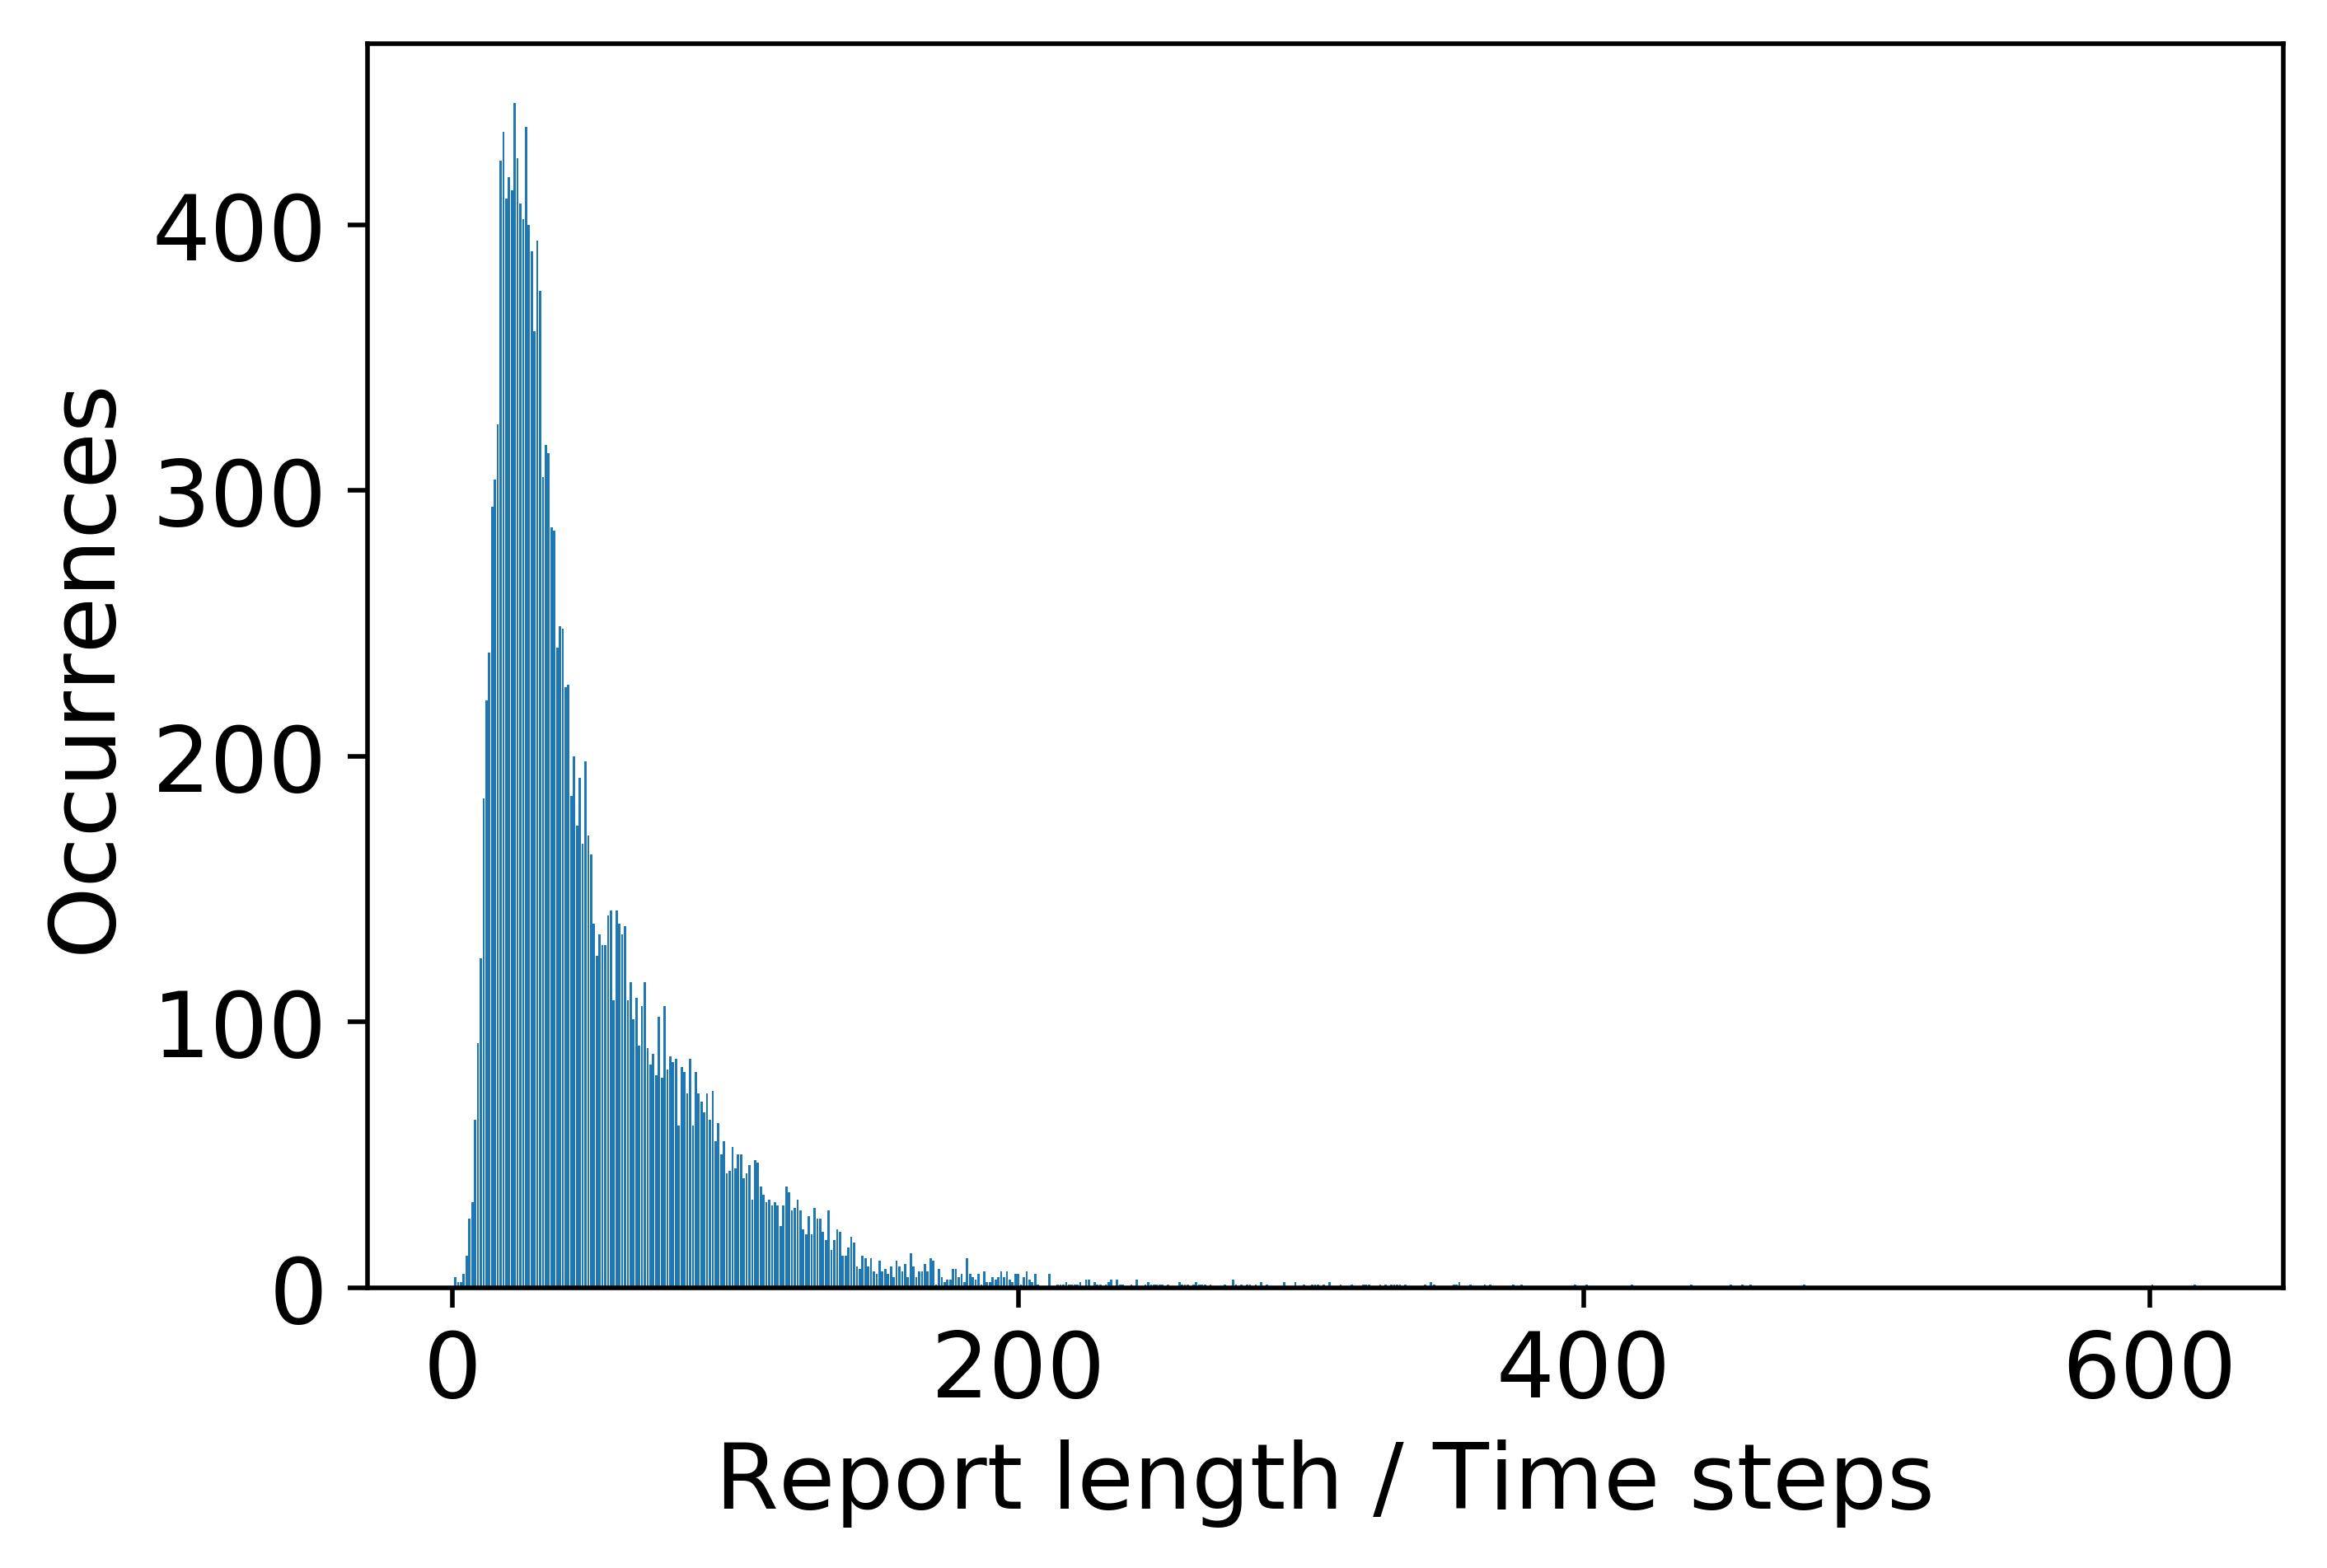
\includegraphics[width=0.5\textwidth]{figures/charts/timesteps_distribution.png}
    \caption{The number of reports per report length}
    \label{figure:timesteps_distribution}
\end{figure}
A view on the lengths of the reports shows (Figure \ref{figure:timesteps_distribution}), that 99.8\% of the reports have a length of 300 or less sequences.
Therefore, for the first architecture 300 \ac{BLSTM} units were used on the first layer for each direction of the \acl{BLSTM}.

Architecture 1:
\begin{addmargin}[1em]{1em}
    \begin{description}
        \item Layer 1: \acl{BLSTM} with 300 units per direction
        \item Layer 2: \acl{BLSTM} with 30 units per direction
        \item Layer 3: \acl{BLSTM} with 3 units per direction
        \item Layer 4: GlobalAveragePooling1D layer to average the different timesteps of the previous \ac{BLSTM} layer
        \item Layer 5: Dense layer with one unit and sigmoid activation
    \end{description}
\end{addmargin}
\begin{figure}[h]
    \centering
    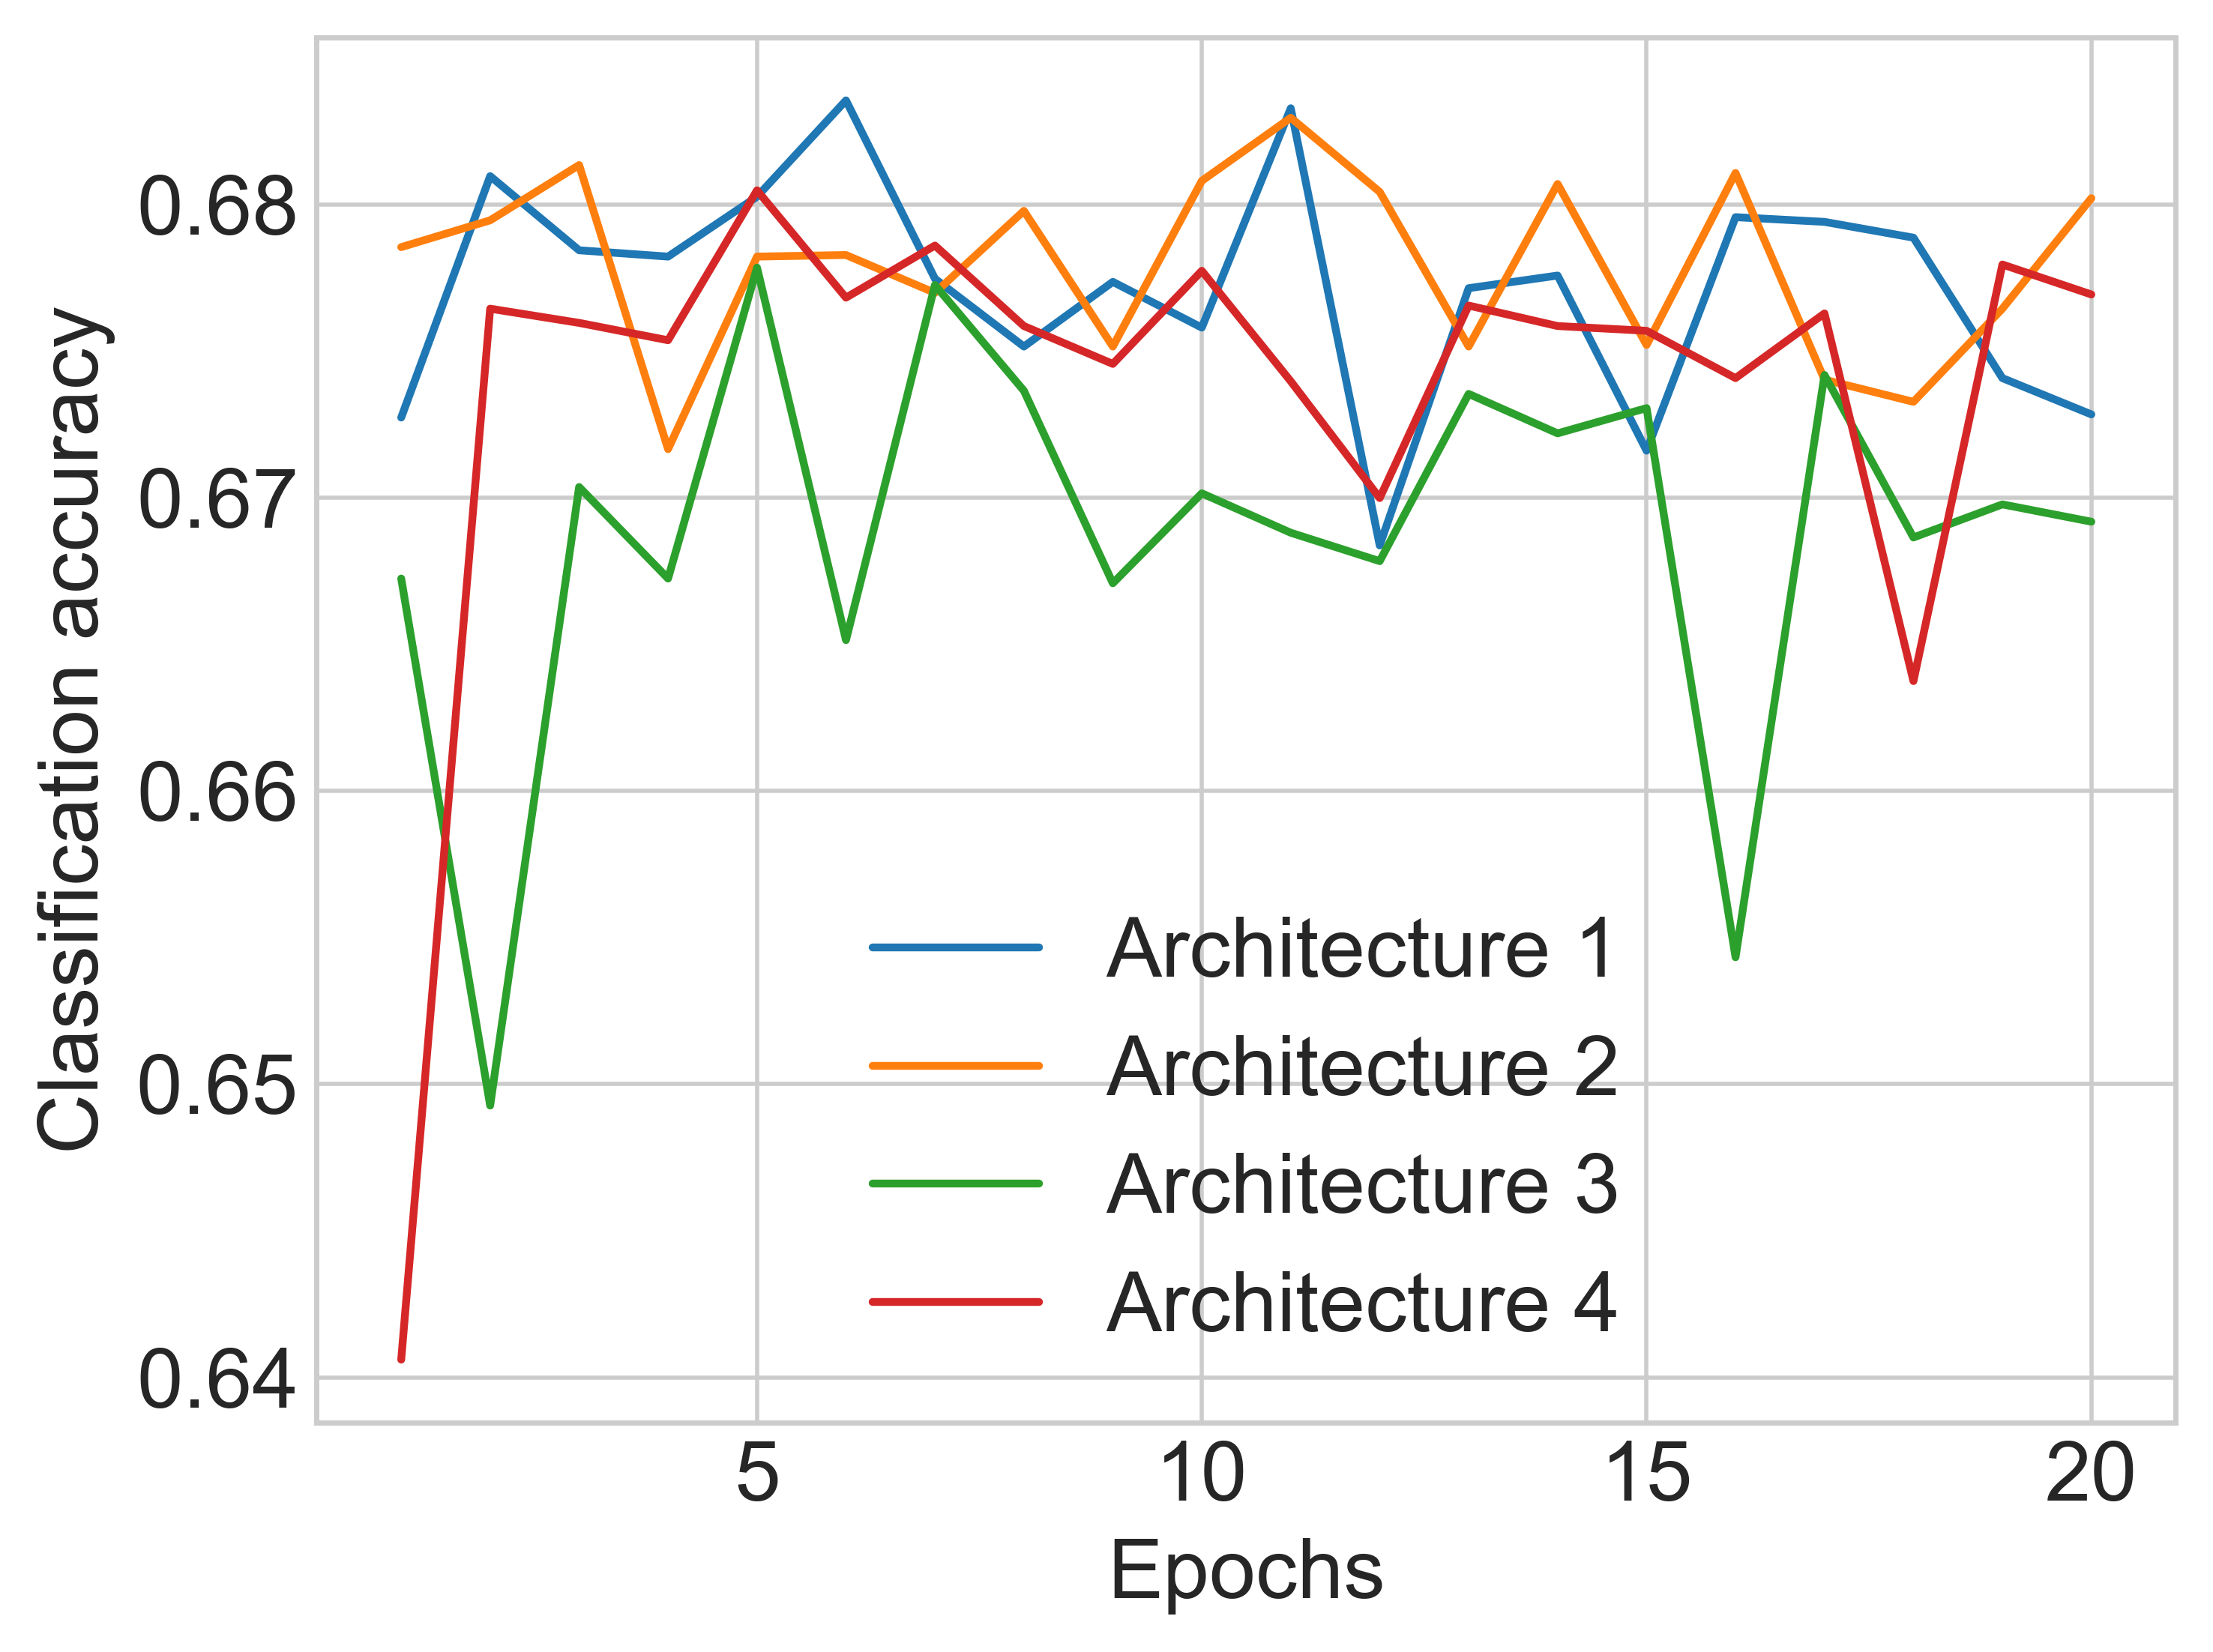
\includegraphics[width=0.5\textwidth]{figures/charts/lstm_learning_curve.png}
    \caption{Learning curves for the different \acl{BLSTM} architectures}
    \label{figure:lstm_learning}
\end{figure}
The learning curve in \ref{figure:lstm_learning} shows no improvement to the classification accuracy compared to the previous experiments.
The other tested architectures did not show any improvement either.
They had the following architectures:

Architecture 2:
\begin{addmargin}[1em]{0em}
    \begin{description}
        \item Layer 1: Bidirectional LSTM with 616 units per direction
        \item Layer 2: Bidirectional LSTM with 62 units per direction
        \item Layer 3: Bidirectional LSTM with 6 units per direction
        \item Layer 4: GlobalAveragePooling layer to average the different timesteps of the previous Bi-LSTM layer
        \item Layer 5: Dense layer with one unit and sigmoid activation
    \end{description}
\end{addmargin}

Architecture 3:
\begin{addmargin}[1em]{0em}
    \begin{description}
        \item Layer 1: Bidirectional LSTM with 616 units per direction
        \item Layer 2: GlobalAveragePooling layer to average the different timesteps of the previous Bi-LSTM layer
        \item Layer 3: Dense layer with 1232 units and sigmoid activation
        \item Layer 4: Dense layer with 120 units and sigmoid activation
        \item Layer 5: Dense layer with 12 units and sigmoid activation
        \item Layer 6: Dense layer with one unit and sigmoid activation
    \end{description}
\end{addmargin}

Architecture 4:
\begin{addmargin}[1em]{1em}
    \begin{description}
        \item Layer 1: Bidirectional LSTM with 500 units per direction
        \item Layer 2: GlobalAveragePooling layer to average the different timesteps of the previous Bi-LSTM layer
        \item Layer 3: Dense layer with 1000 units and sigmoid activation
        \item Layer 4: Dense layer with 100 units and sigmoid activation
        \item Layer 5: Dense layer with 10 units and sigmoid activation
        \item Layer 6: Dense layer with one unit and sigmoid activation
    \end{description}
\end{addmargin}
The 616 units on the first layer of Architecture 2 and 3 was chosen because, the maximum length of the reports were 616 sequences (figure \ref{figure:timesteps_distribution}).
Since none of these architectures outperformes the other architectures significantly, the second architecture was used to obtain a final test accuracy of 68.3\%.
Even though this is a worse result, than what the \ac{SVM} reached, there is still a takeaway from these experiments concerning the LSTM architecture, which is that the models with multiple LSTM layers seem to perform better than the models with a single LSTM layer.


\subsection{Naive Bayes}
The Naive Bayes model did not show a significant improvement, when using the average and the standard deviation of the features.
The learning curve in figure \ref{figure:nb_learning_std} is really similar to the learning curve that was obtained in section \ref{subsec:nb_results}.
\begin{figure}[h]
    \centering
    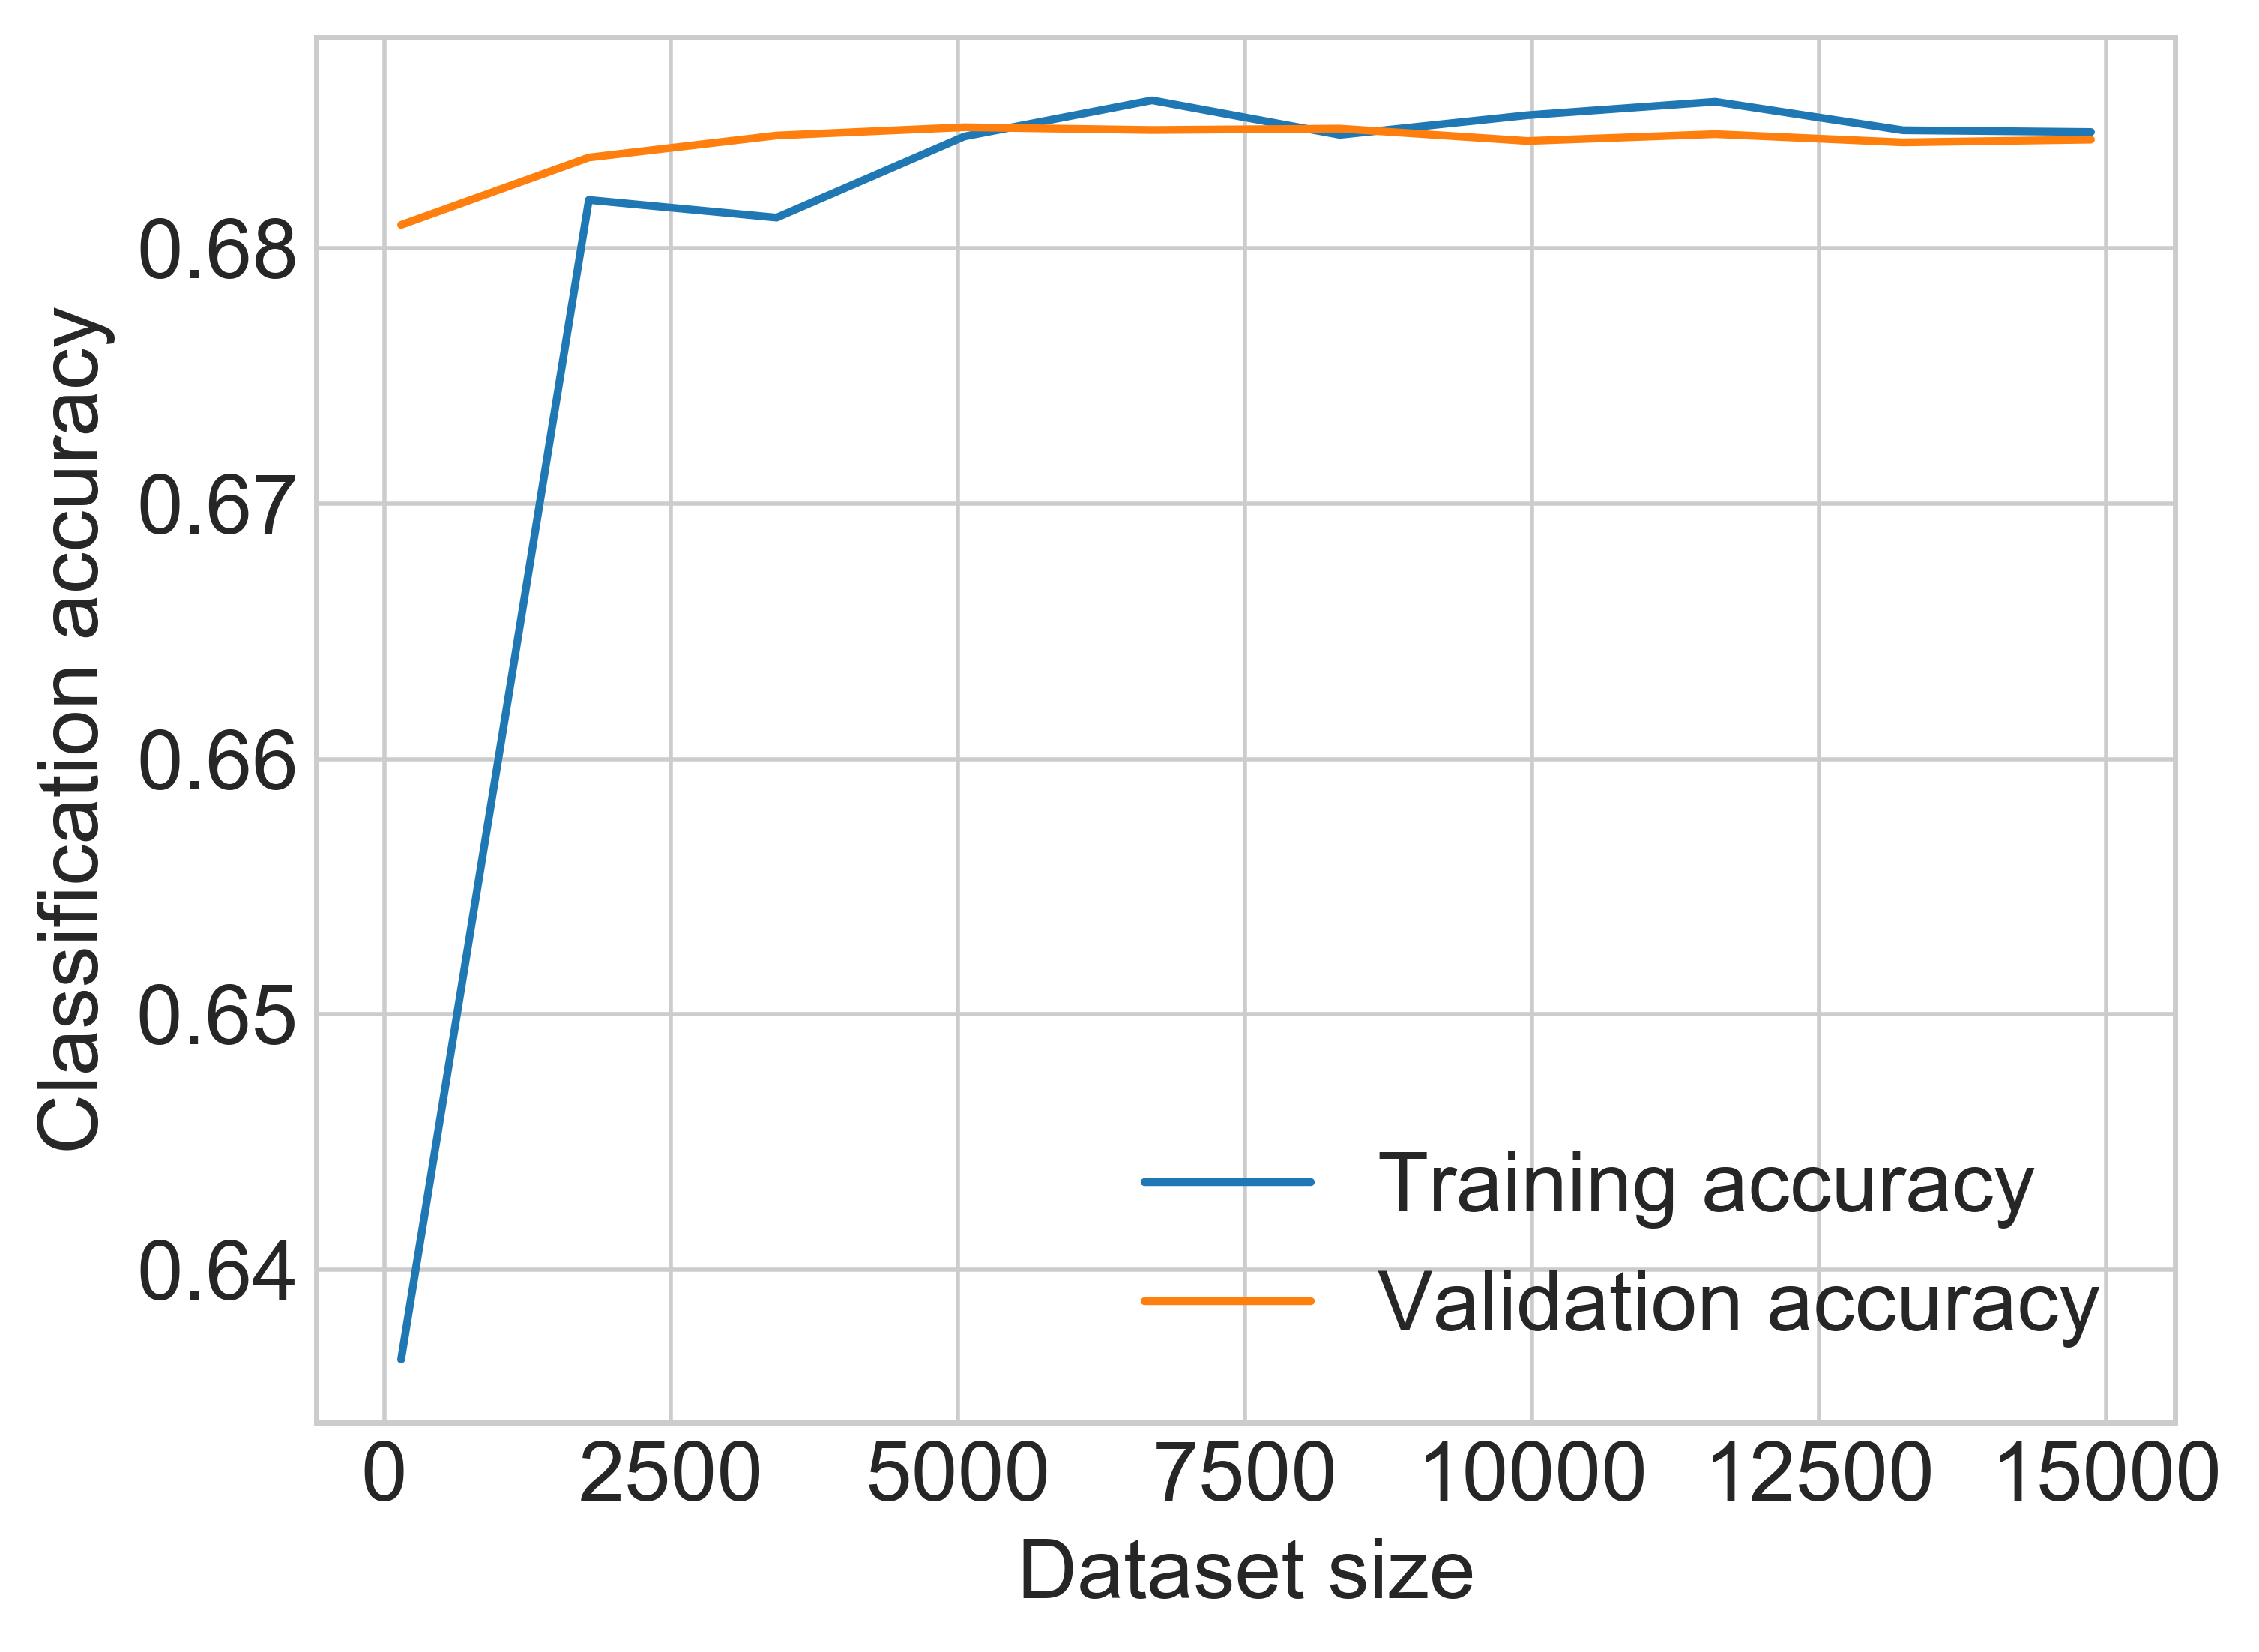
\includegraphics[width=0.5\textwidth]{figures/charts/training_with_std/nb_learning.png}
    \caption{Learning curve of the Naive Bayes classifier when the averages and the standard deviation of the sequence embeddings are used.}
    \label{figure:nb_learning_std}
\end{figure}
Since it has a small slope at large training dataset sizes, the accuracy would also not increase significantly if more data was provided.
The test accuracy was 0.1\% higher, reaching 68.2\% compared to 68.1\% when using only the report averages previously.

\subsection{\acl{KNN} classifier}
Since the input feature vectors with the average and the standard deviation of the sequence embeddings are twice as long as for the previous experiment, the optimal value of $K$ did also change.
The highest cross-validation accuracy was reached at $K=233$ with 68.7\%, as the validation curve in figure \ref{figure:knn_validation_std} shows.
\begin{figure}[h]
    \begin{subfigure}{0.5\textwidth}
        \centering
        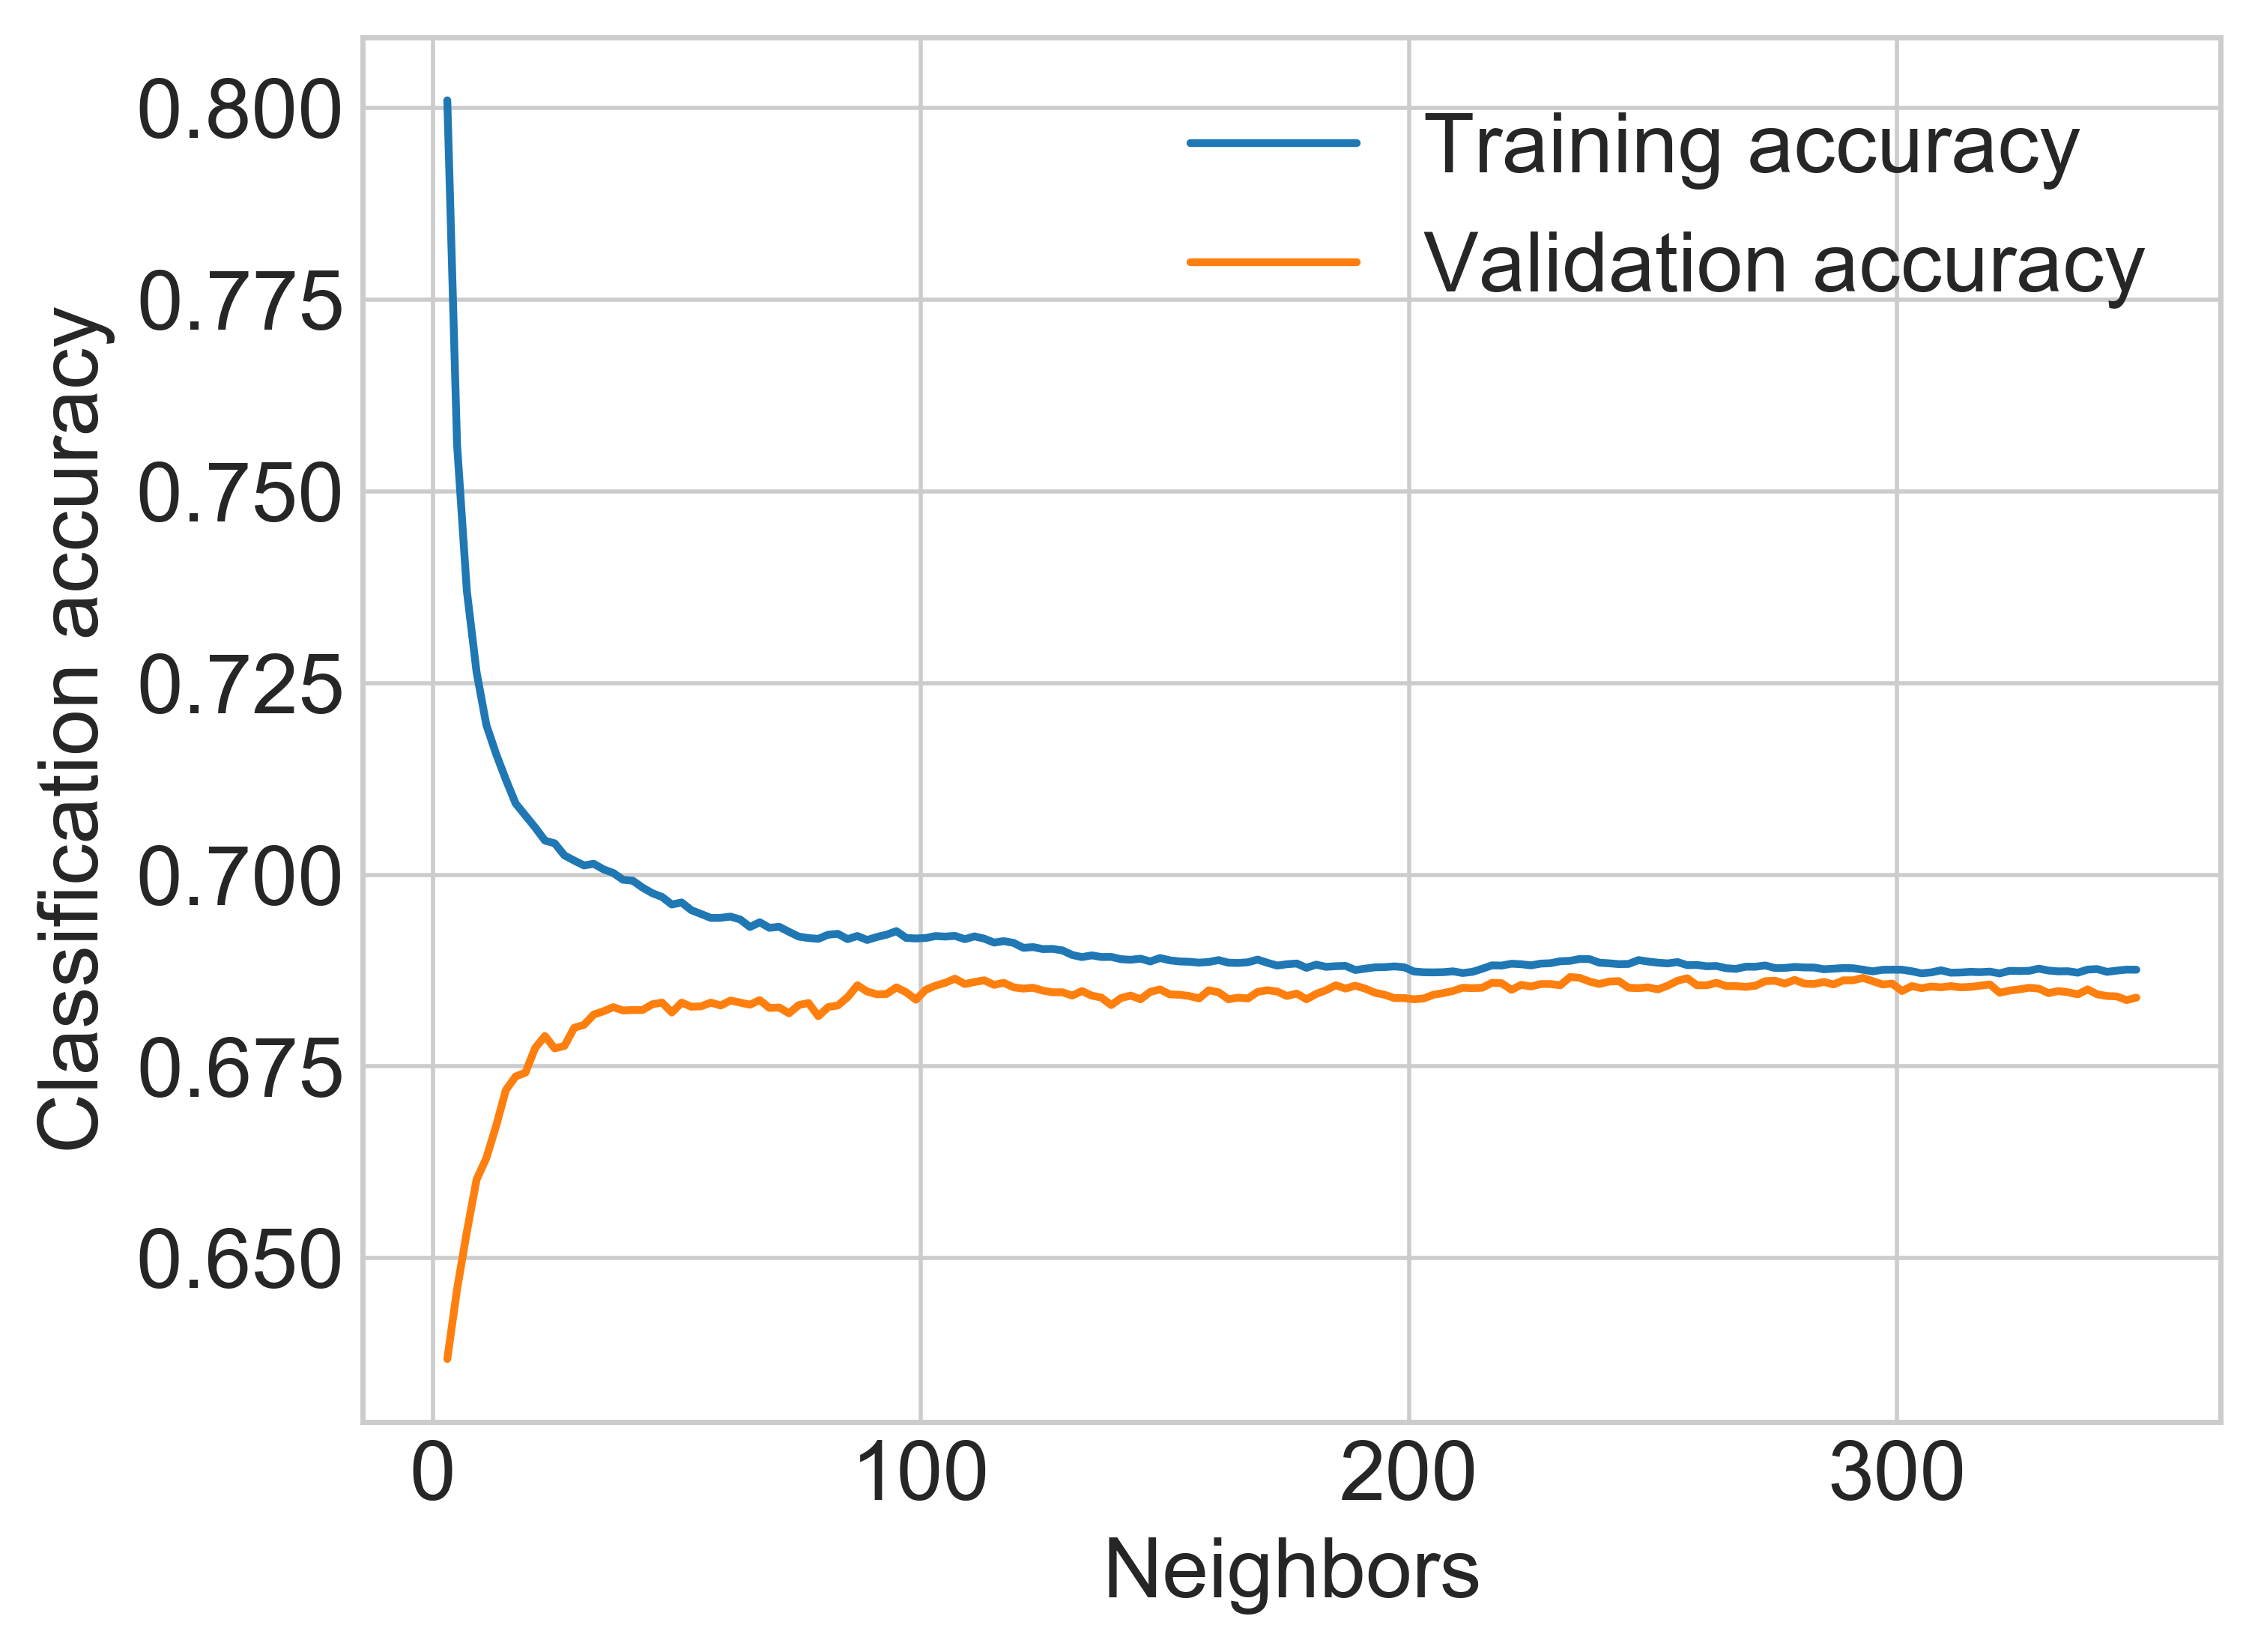
\includegraphics[width=\textwidth]{figures/charts/training_with_std/knn_validation.png}
        \caption{Validation curve.}
        \label{figure:knn_validation_std}
    \end{subfigure}
    \begin{subfigure}{0.5\textwidth}
        \centering
        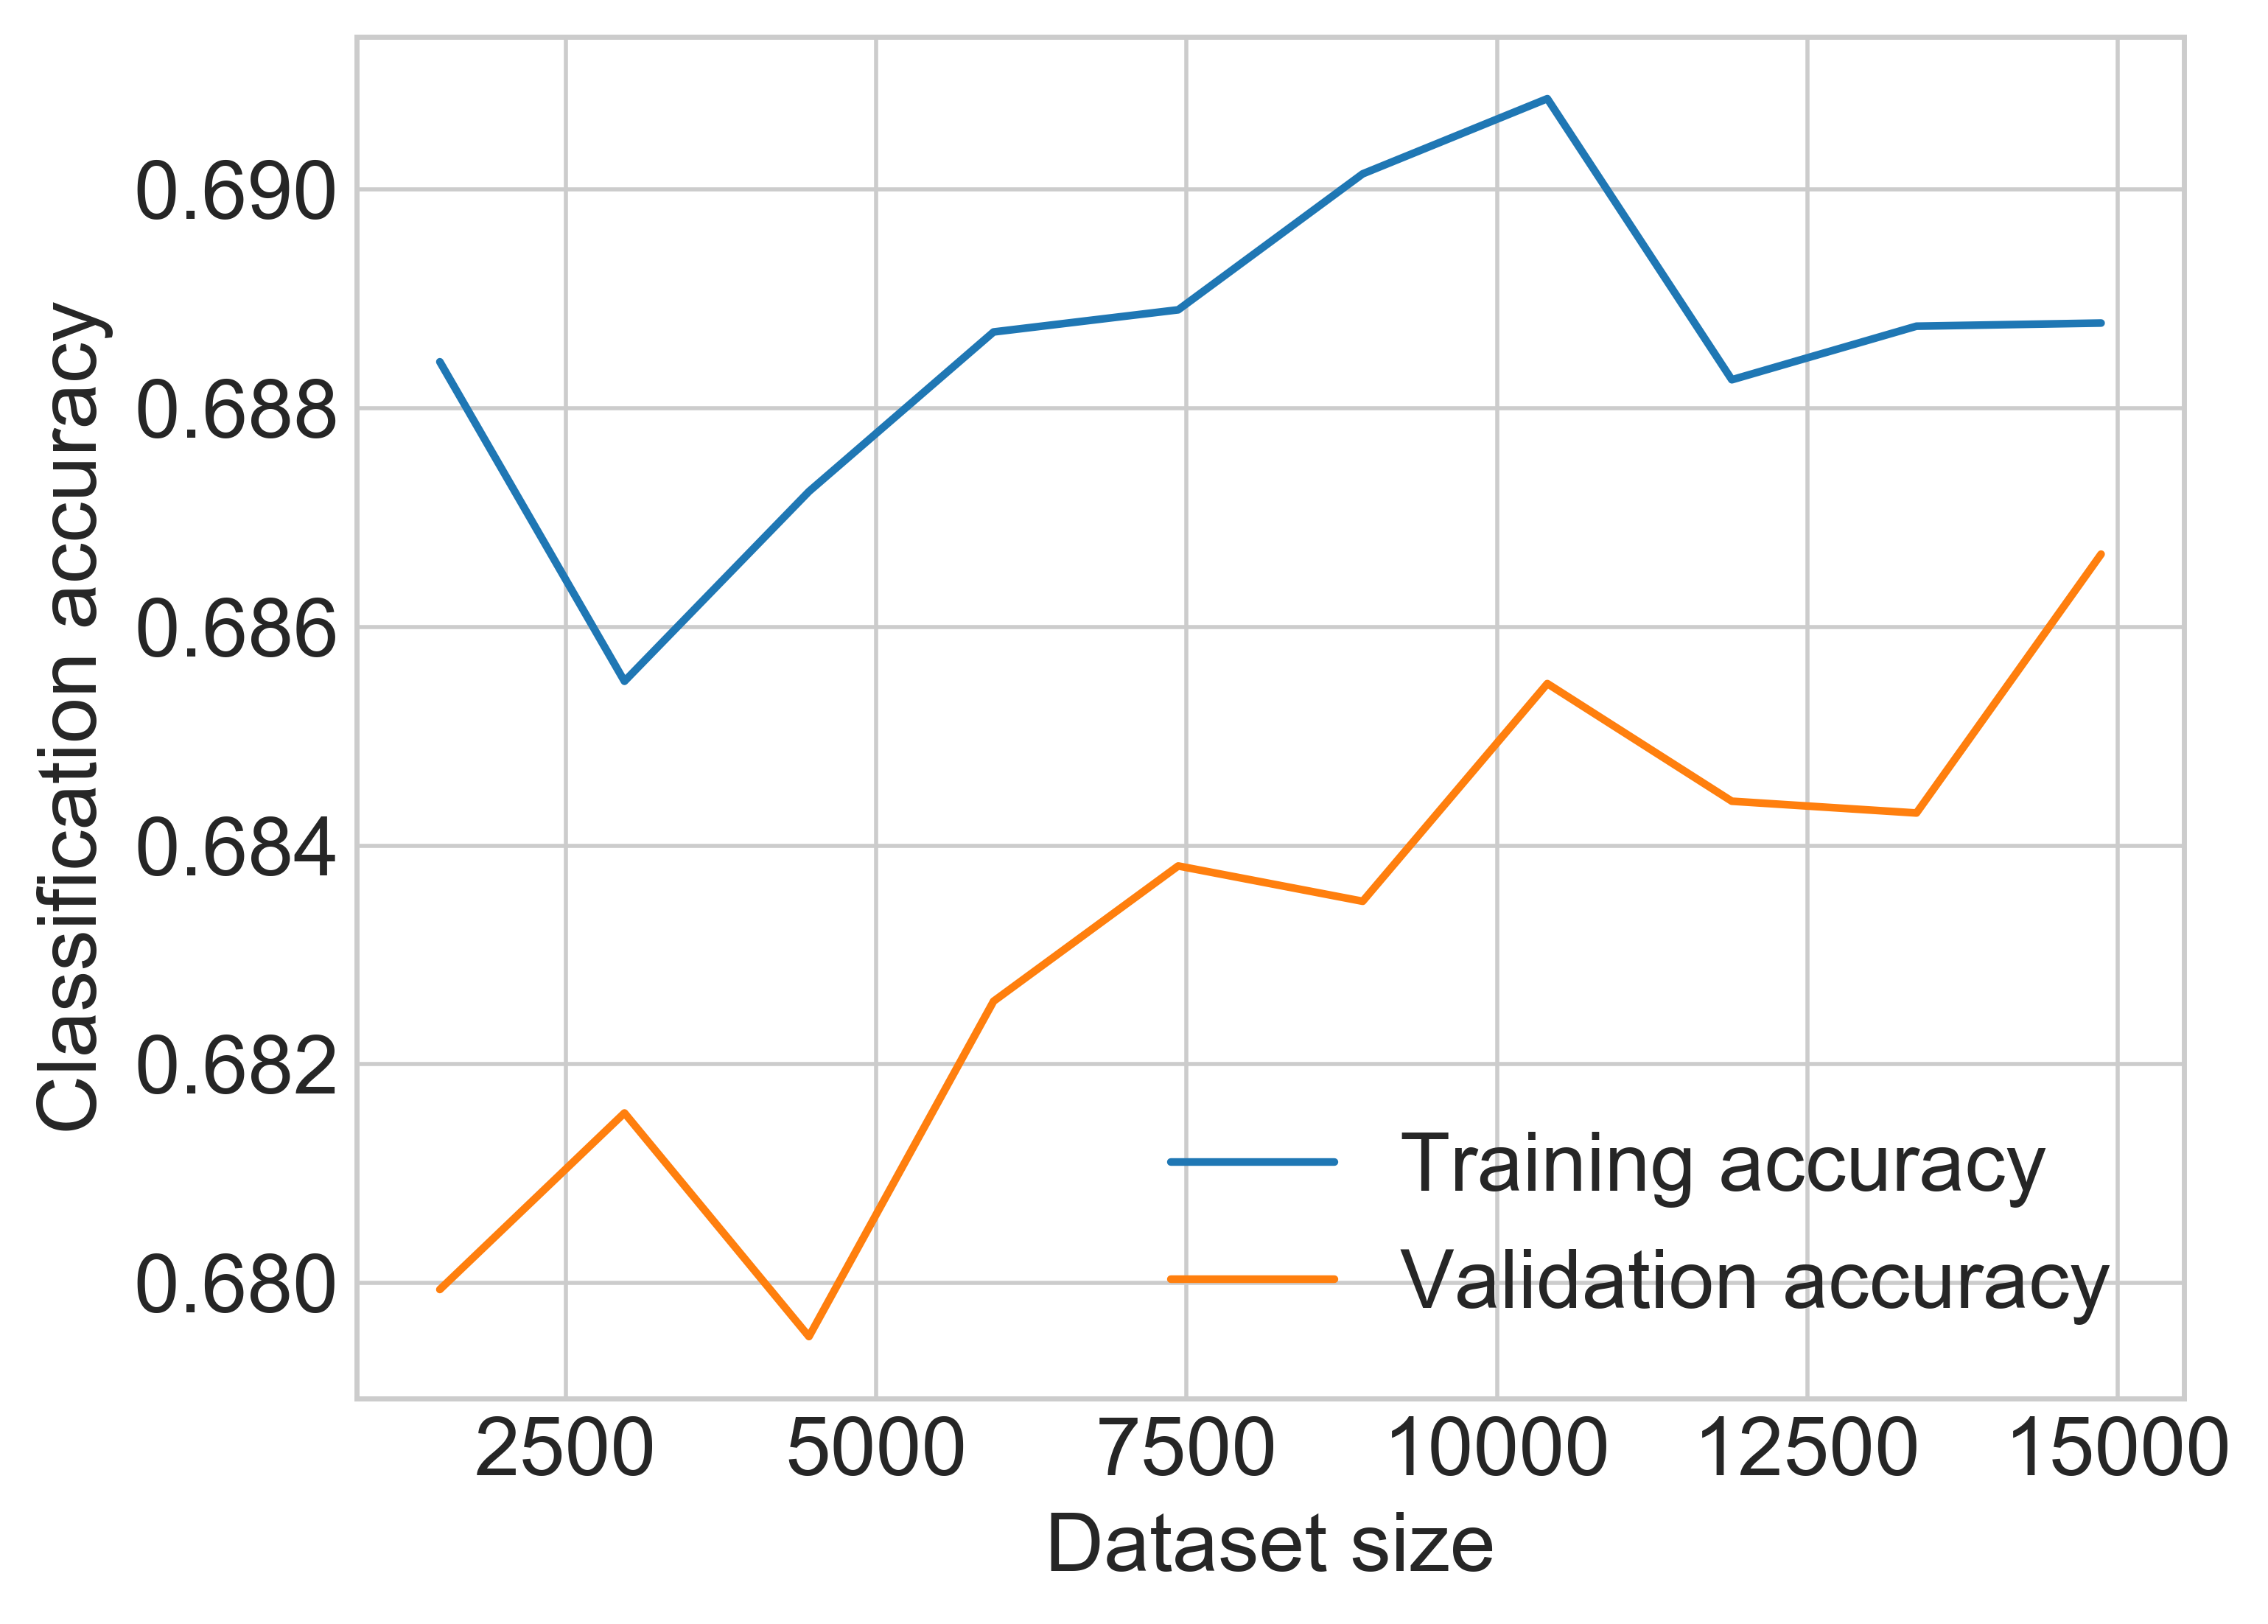
\includegraphics[width=\textwidth]{figures/charts/training_with_std/knn_learning.png}
        \caption{Learning curve for for $K=233$.}
        \label{figure:knn_learning_std}
    \end{subfigure}
    \caption{Validation and learning curve for the k-nearest neighbor classifier when using the average and the standard deviation of the features.}
    \label{figure:knn_std}
\end{figure}
The learning curve in figure \ref{figure:knn_learning_std} suggests again that the model could improve, if more data was available.
The accuracy on the test dataset was 68.3\% which is no improvement to the previous experiment.

\subsection{\acl{SVM}}
For the \ac{SVM} the optimal values of $C$ and $\gamma$ changed as well, as the new validation curves (figure \ref{figure:svm_validation_std}) show.
\begin{figure}[h]
    \begin{subfigure}{0.5\textwidth}
        \centering
        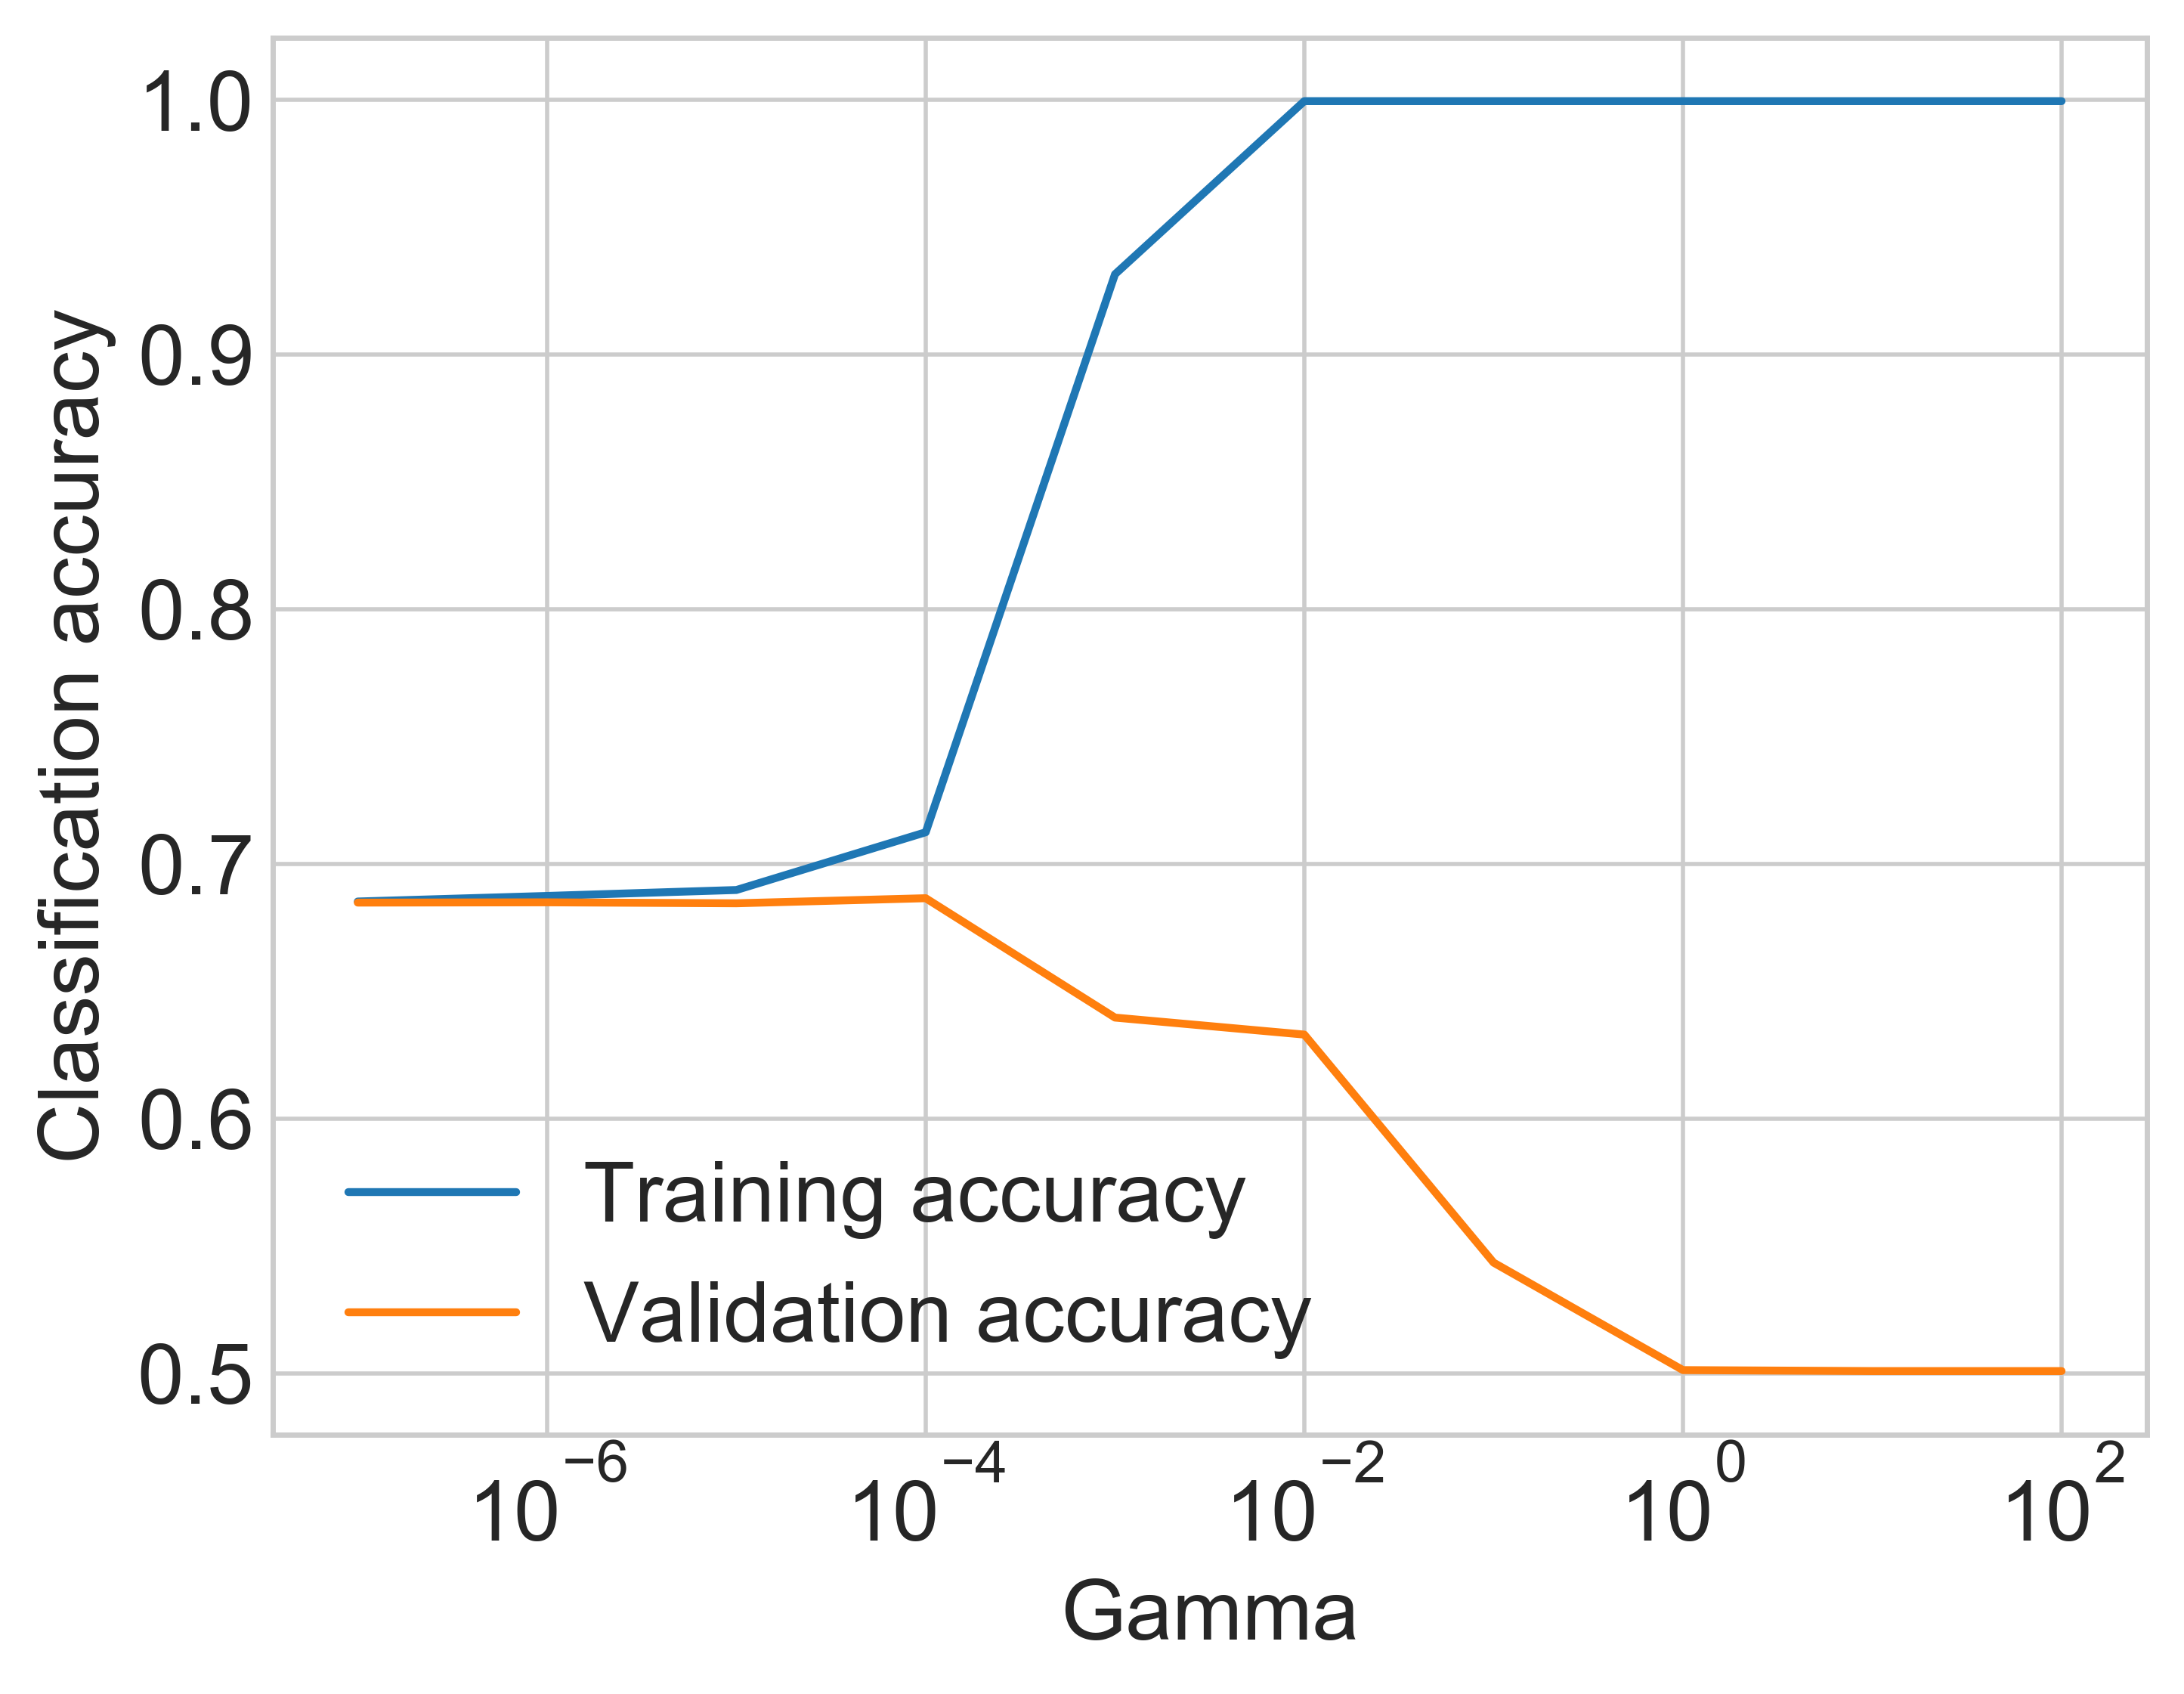
\includegraphics[width=\textwidth]{figures/charts/training_with_std/svm_validation_C_100.png}
        \caption{C=100}
        \label{figure:svm_validation_std_C_100}
    \end{subfigure}
    \begin{subfigure}{0.5\textwidth}
        \centering
        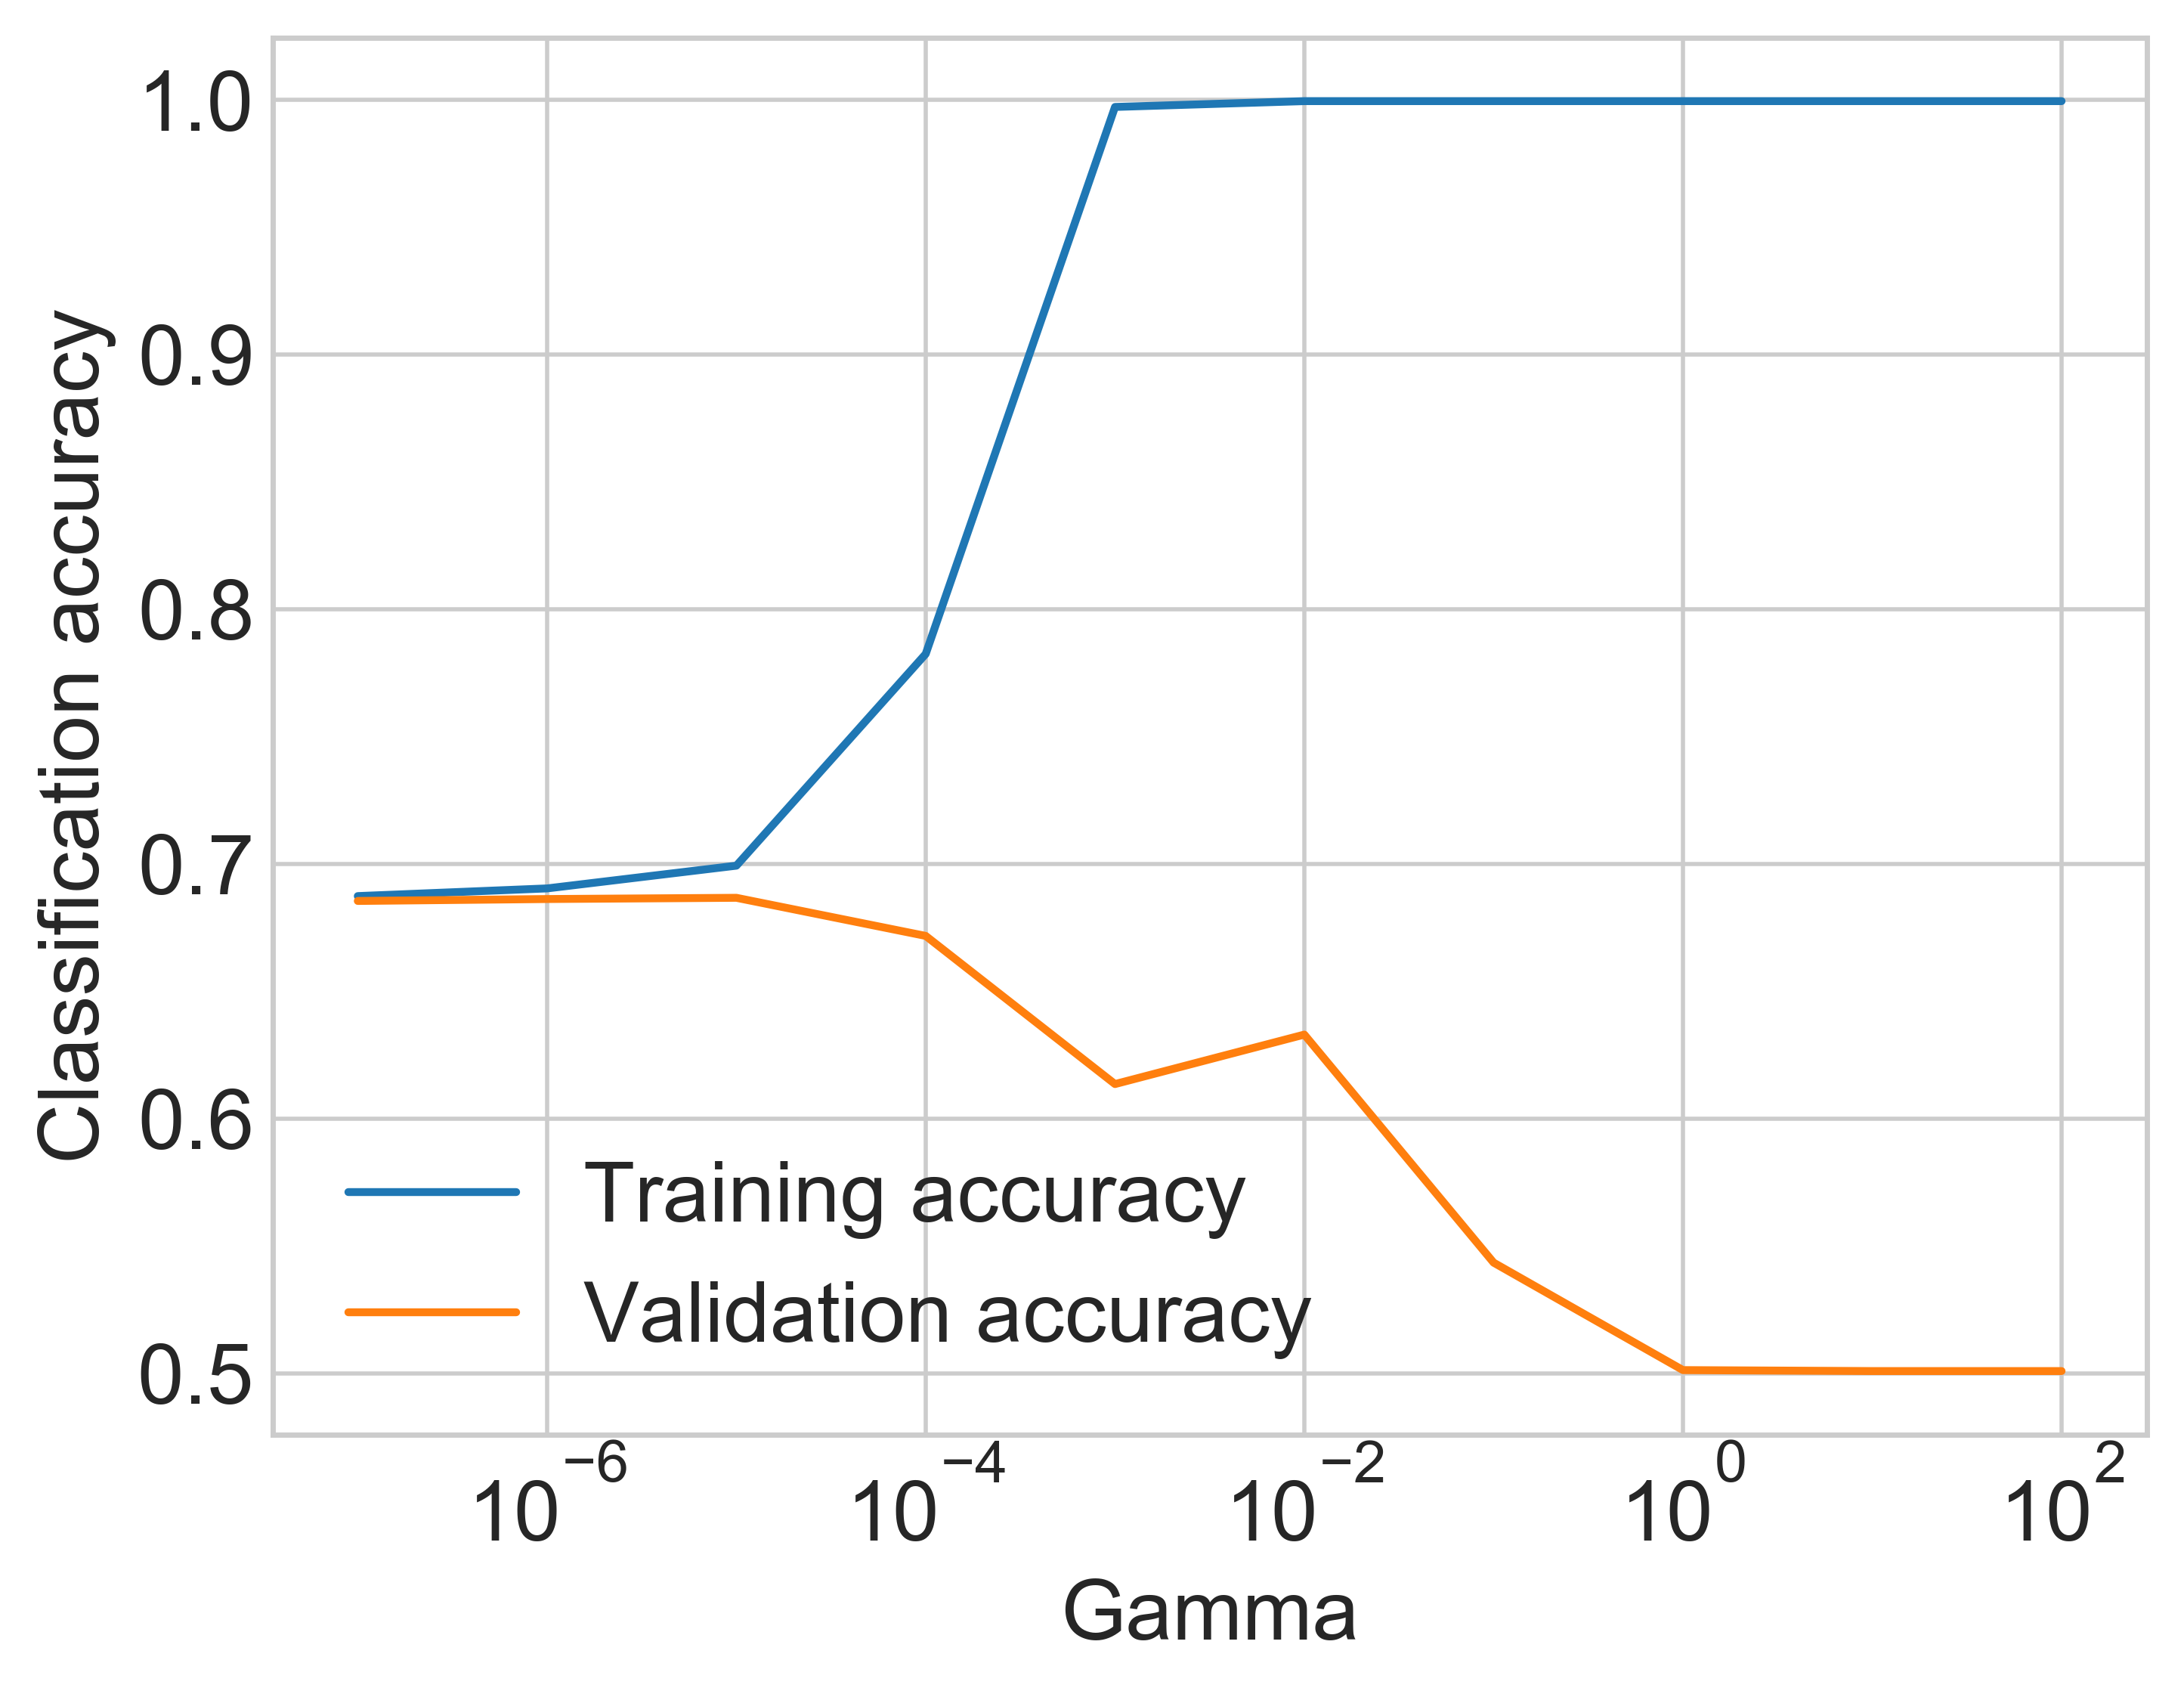
\includegraphics[width=\textwidth]{figures/charts/training_with_std/svm_validation_C_1000.png}
        \caption{C=1000}
        \label{figure:svm_validation_std_C_1000}
    \end{subfigure}
    \begin{subfigure}{0.5\textwidth}
        \centering
        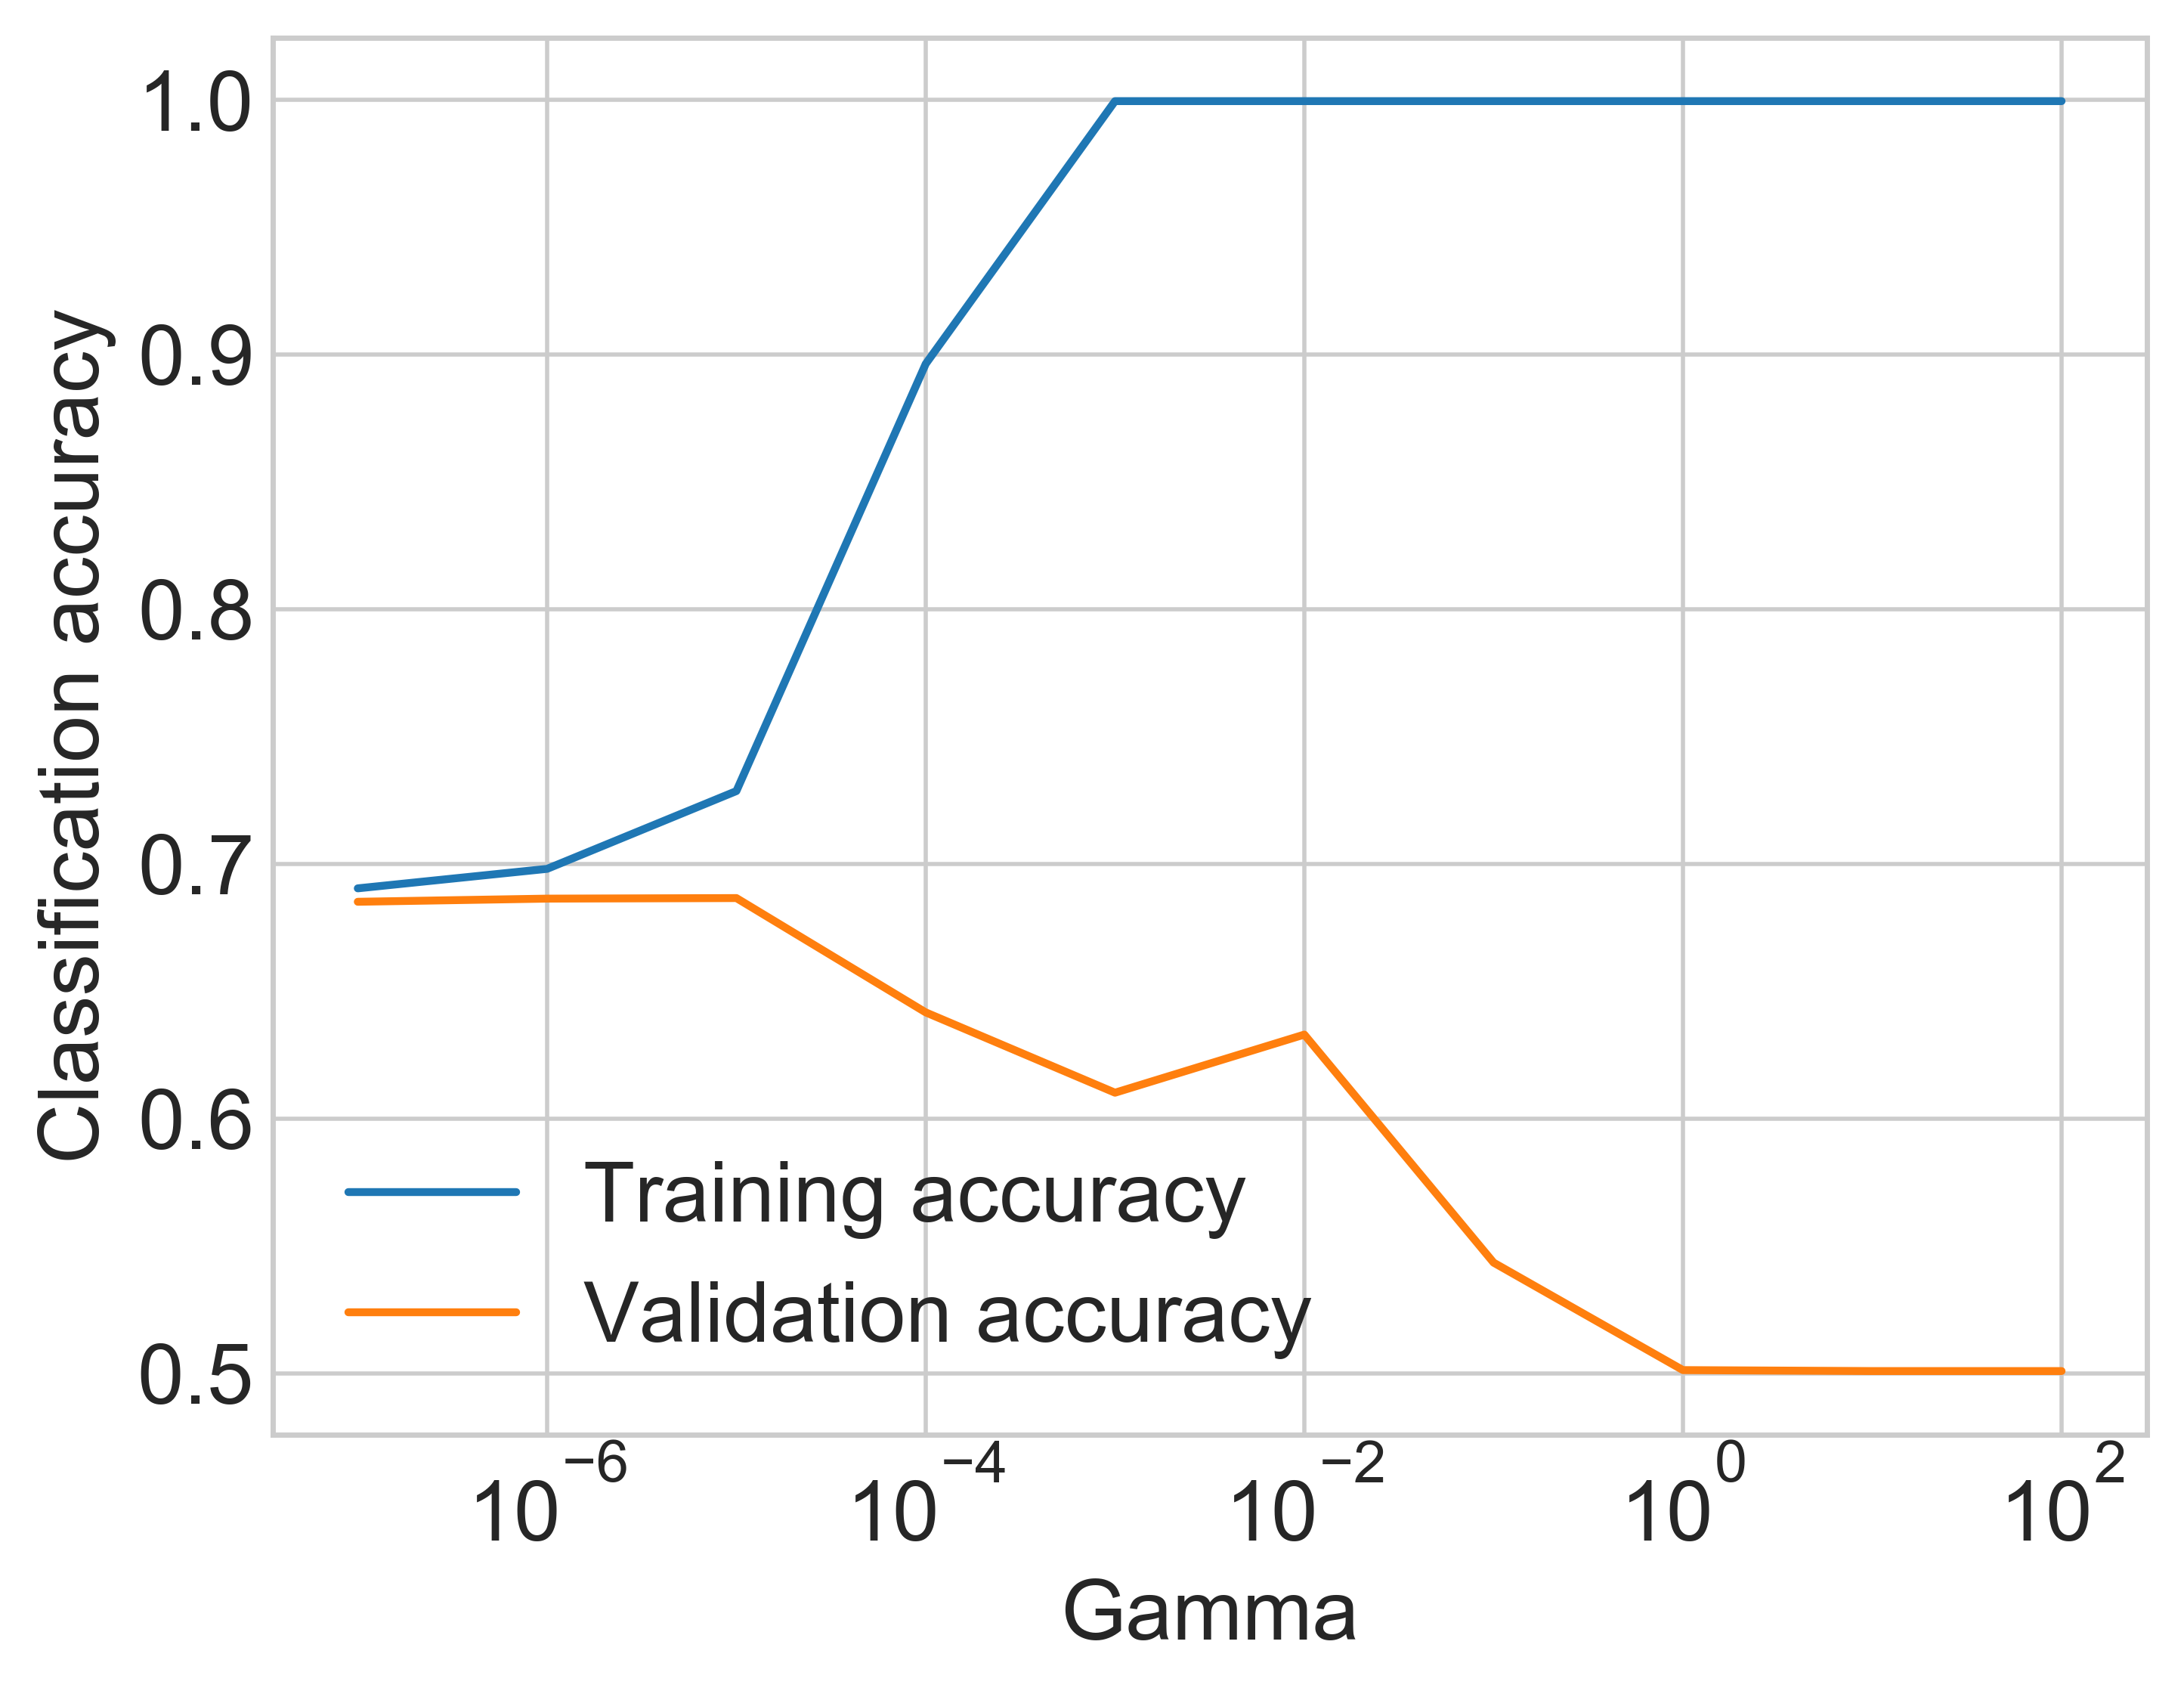
\includegraphics[width=\textwidth]{figures/charts/training_with_std/svm_validation_C_10000.png}
        \caption{C=10000}
        \label{figure:svm_validation_std_C_10000}
    \end{subfigure}
    \begin{subfigure}{0.5\textwidth}
        \centering
        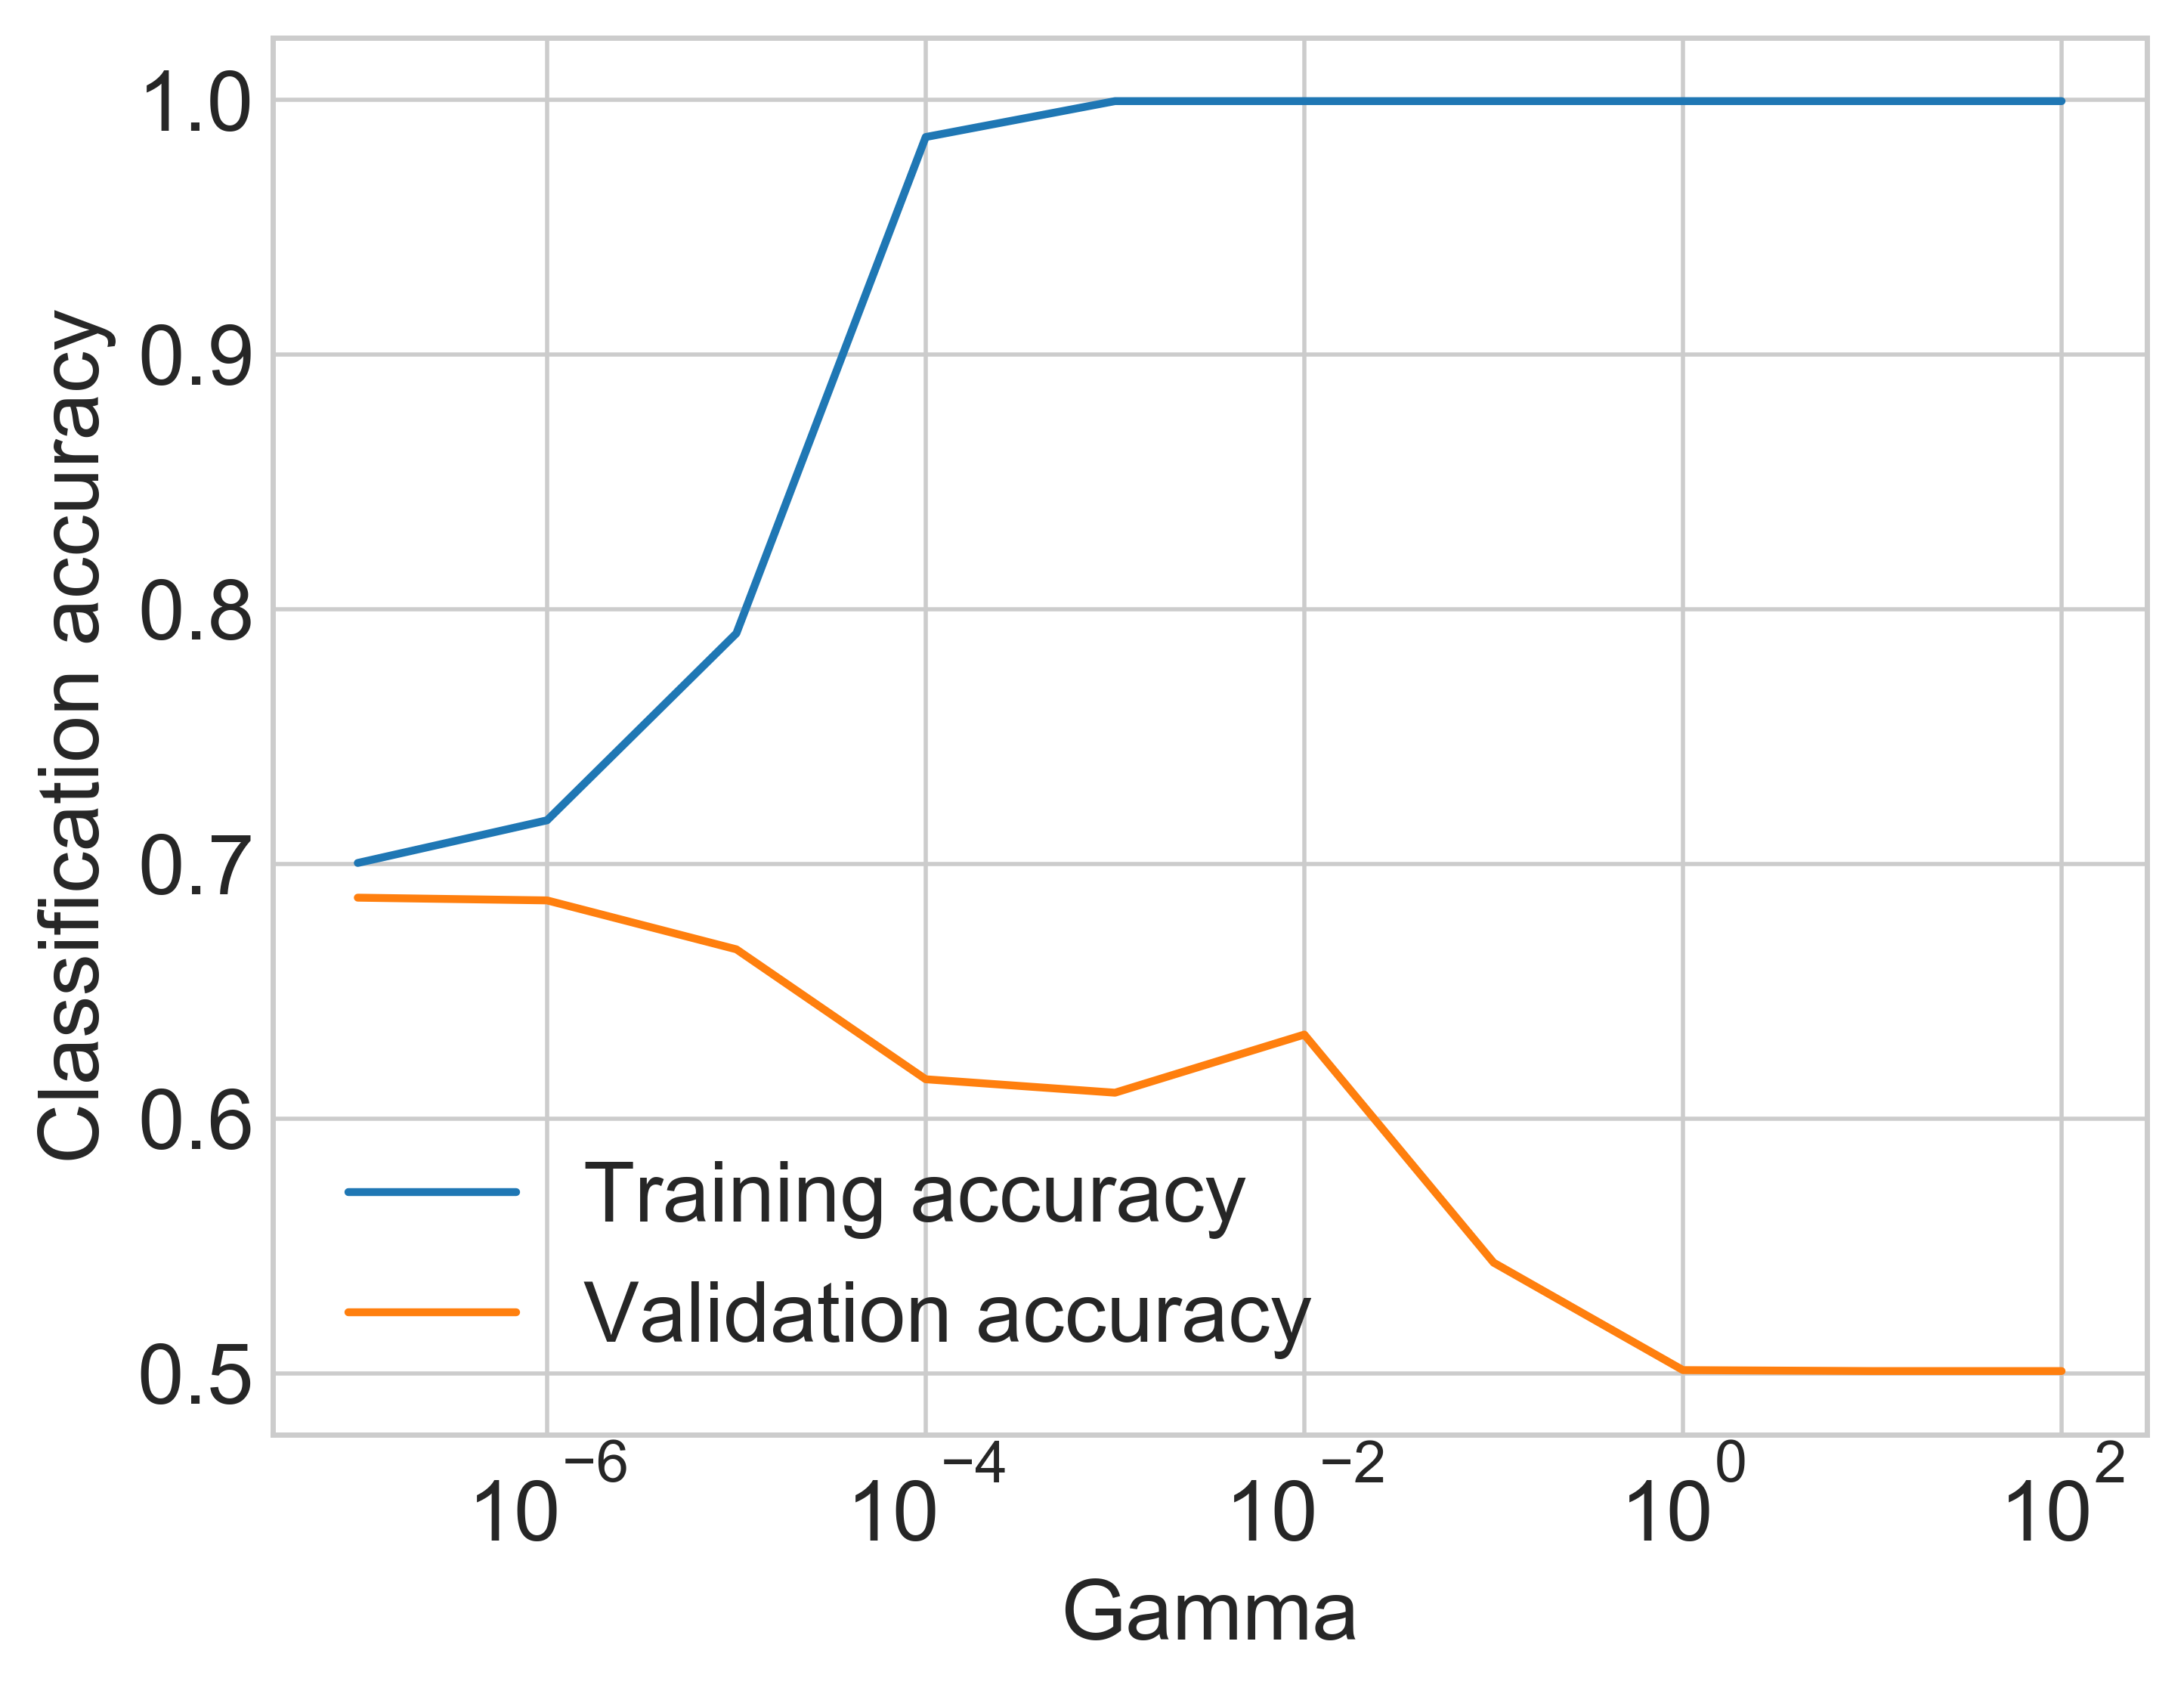
\includegraphics[width=\textwidth]{figures/charts/training_with_std/svm_validation_C_100000.png}
        \caption{C=100000}
        \label{figure:svm_validation_std_C_100000}
    \end{subfigure}
    \caption{Validation curves for different values of C when using the average and the standard deviation of the features.}
    \label{figure:svm_validation_std}
\end{figure}
The highest accuracy is now reached at $C=100000$ and $\gamma$ set to $1\cdot10^{-7}$ with 68.7\% on the validation dataset.
These hyperparameters lead to the learning curve in figure \ref{figure:svm_learning_std}.
\begin{figure}[h]
    \centering
    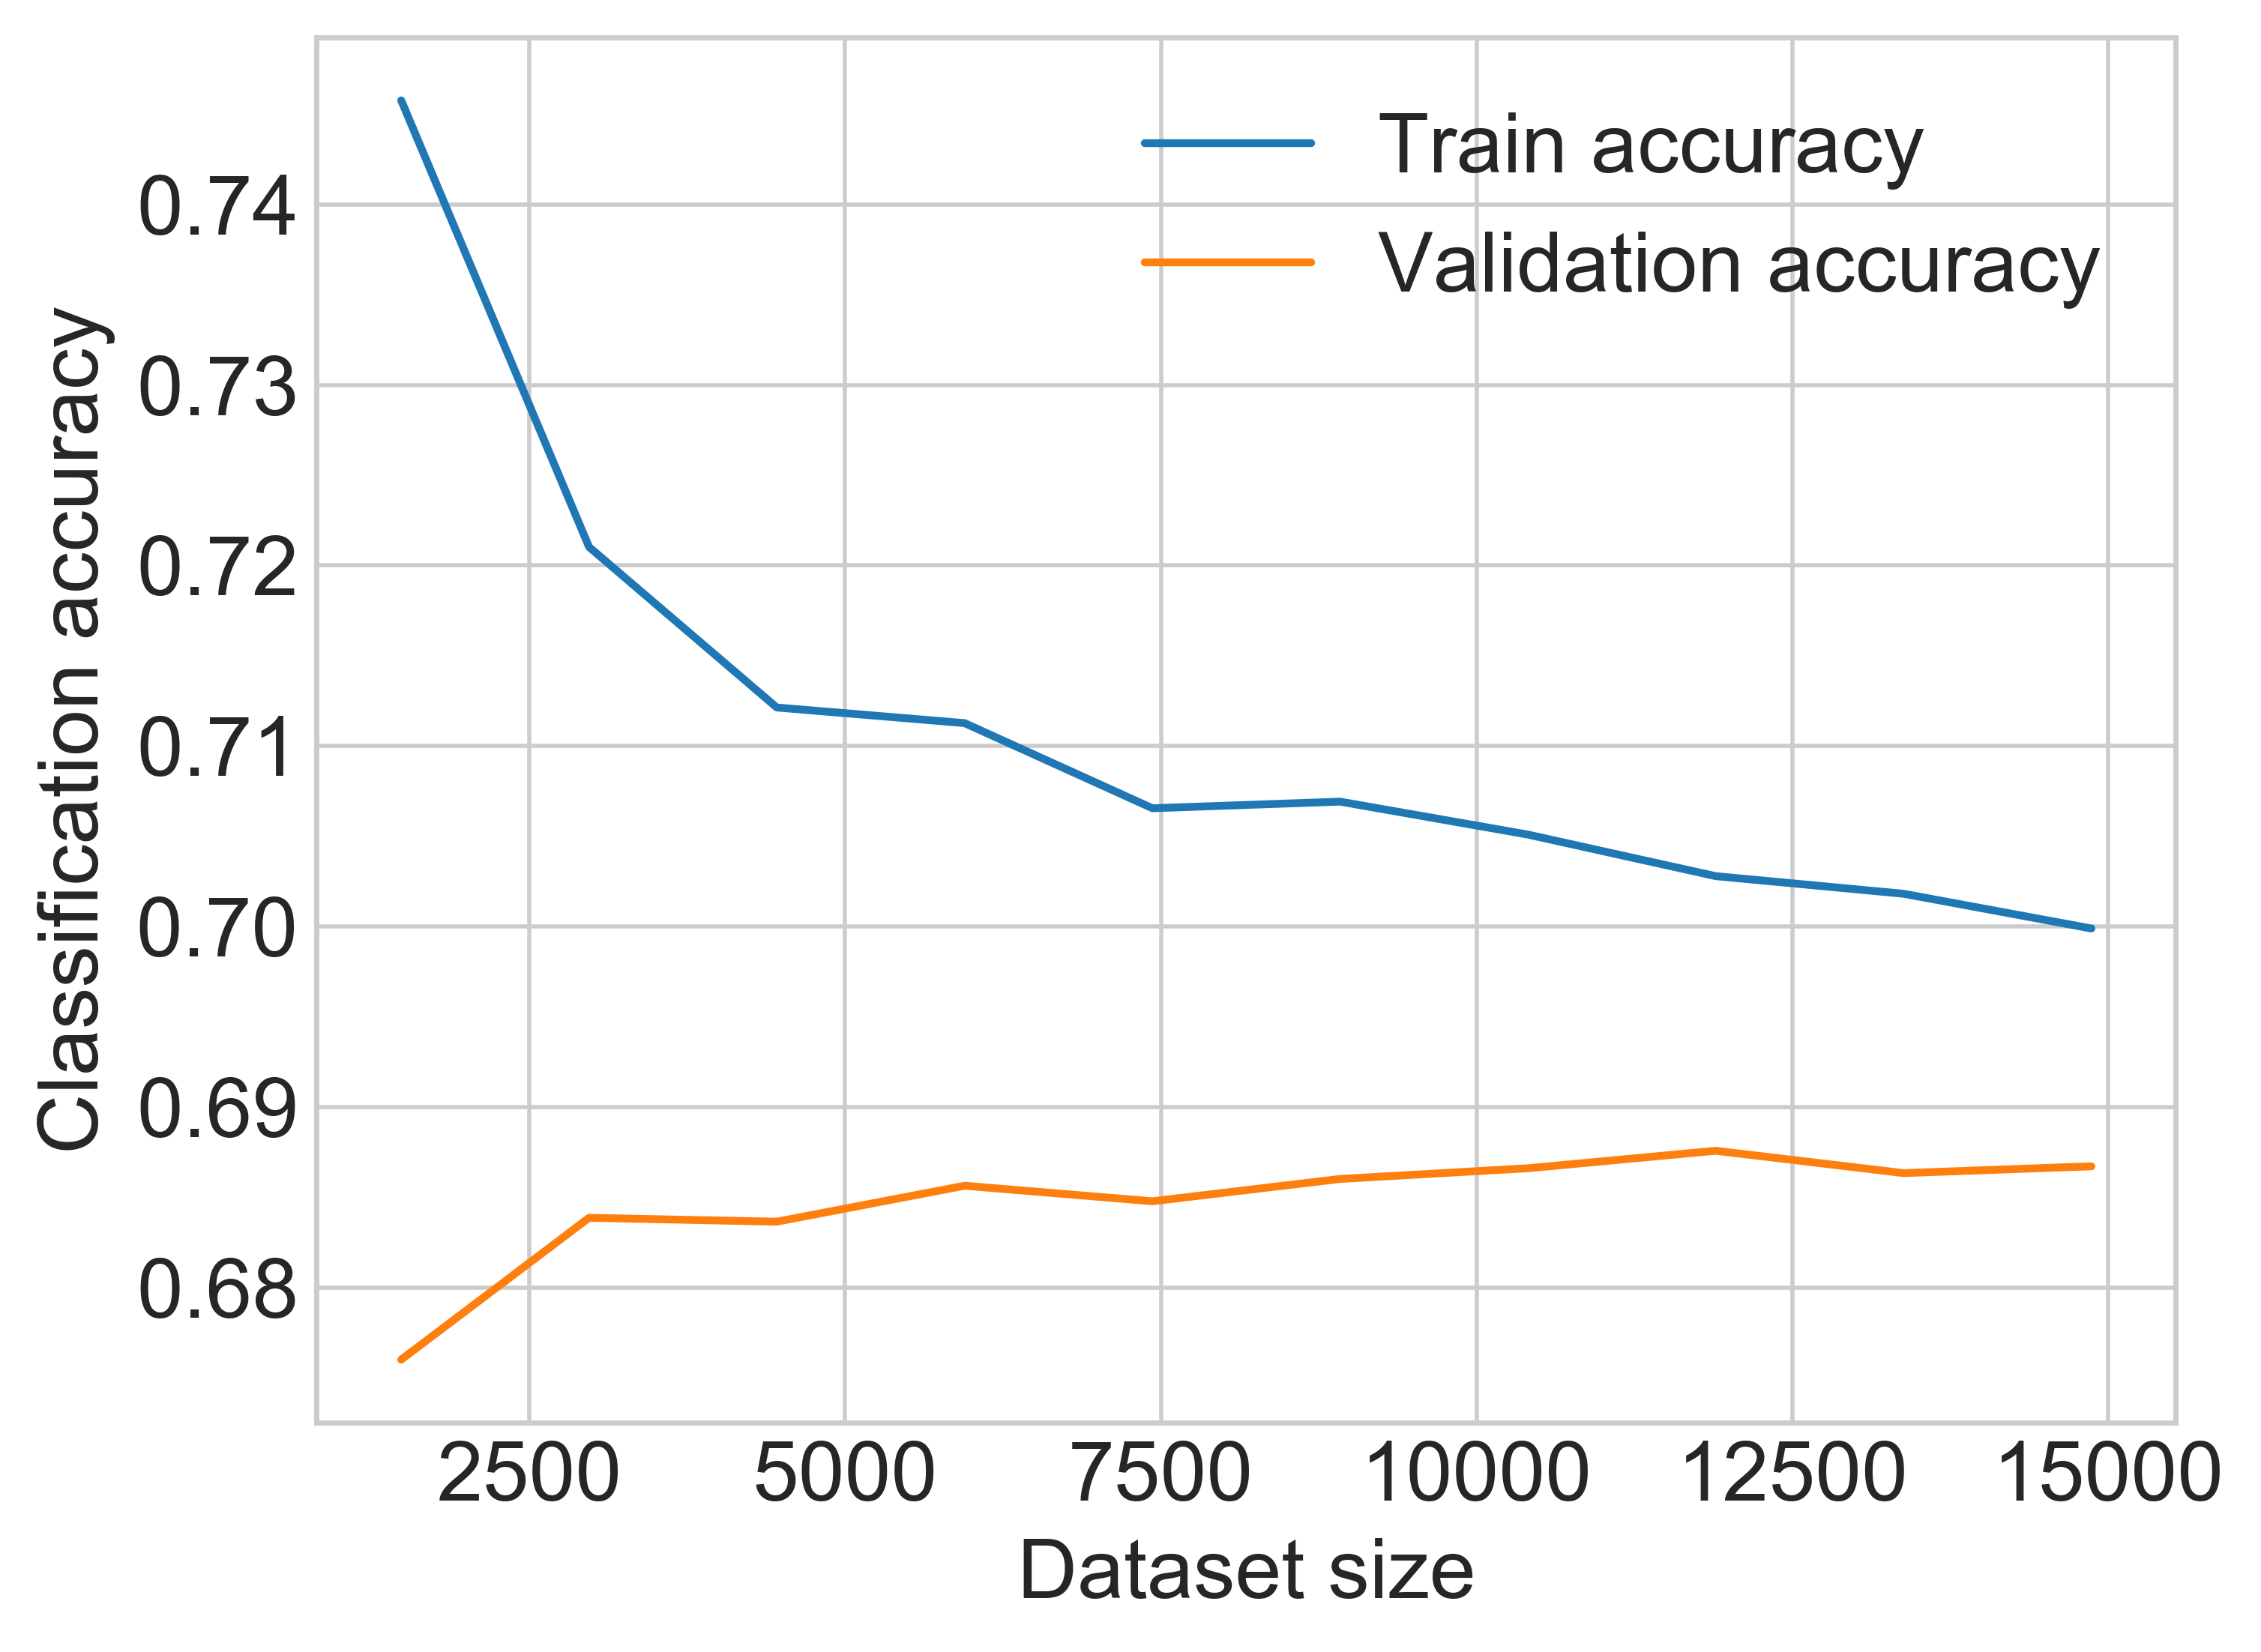
\includegraphics[width=0.5\textwidth]{figures/charts/training_with_std/svm_learning_curve.png}
    \caption{Learning curve for the \ac{SVM} with $C=100000$ and $\gamma=1\cdot10^{-7}$.}
    \label{figure:svm_learning_std}
\end{figure}
The \ac{SVM} with $C=100000$ and $\gamma=1\cdot10^{-7}$ reached a test accuracy of 69.1\%, which is worse than the 69.3\% accuracy that was reached, when only using the averages of the features.

Table \ref{table:test_results} summarizes the test results of the classifiers.
As it can be seen all classifiers performed approximatly similar, however the \ac{SVM} clearly achieved the best accuracy at 69.3\% with the hyperparameters $C=100$ and $\gamma=0.0001$.
\begin{table}[h]
    \begin{tabular}{ c | c | c || c || c | c | c }
        \multicolumn{3}{c||}{Features average} & Features sequential & \multicolumn{3}{c}{Features average and standard deviation} \\ \hline
        Naive bayes & KNN & SVM & Bi-LSTM & Naive bayes & KNN & SVM \\ \hline
        68.1\% & 68.3\% & \textbf{69.3\%} & 68.3\% & 68.2\% & 68.3\% & 68.7\% 
        % & \multirow{5}{*}{-} & \multirow{5}{*}{$K = 111$} & & $2\times616$ LSTM units & \multirow{5}{*}{-} & \multirow{5}{*}{$K=233$} & \\
        % Configuration/ & & $C=100$, & & $2\times62$ LSTM units & & & $C=100000$, \\
        % Hyperparameters& & $\gamma=0.0001$ & & $2\times6$ LSTM units & & & $\gamma=1\cdot10^{-7}$ \\
        % & & & & GlobalAveragePooling & & & \\
        % & & & & $1$ Dense (sigmoid activation) & & & 
    \end{tabular}
    \caption{Test accuracies of the different classifiers.}
    \label{table:test_results}
\end{table}



% Two other configurations were tested as well: An increase in the amount of warmup steps to 92500 did not show any improvement (yellow curve) in the Masked LM Accuracy, just as little as using a modified vocabulary.
% The idea behind the modified vocabulary is

